\documentclass[journal]{IEEEtran}
%\documentclass[journal,a5paper]{IEEEtran}
\usepackage[a5paper, margin=10mm]{geometry}
\setlength{\headheight}{1cm} % Set the height of the header box
\setlength{\headsep}{0mm}     % Set the distance between the header box and the top of the text
\usepackage{gvv-book}
\usepackage{gvv}

\makeindex

\begin{document}
\bibliographystyle{IEEEtran}
\onecolumn


\title{
	\begin{center}
Digital Design Through Arduino
%	\\
%\rule{0.4\columnwidth}{0.4pt}
\end{center}
}
\author{
\vspace{11cm}
	\begin{center}
\includegraphics[width=0.2\columnwidth]{figs/logo.jpg}
\\
%\hfill
		{\huge	G. V. V. Sharma}\\Associate Professor,\\Department of Electrical Engineering, \\ IIT Hyderabad
	\end{center}
%\IEEEpubid{\makebox[\columnwidth]{978-1-7281-5966-1/20/\$31.00 ©2020 IEEE \hfill} \hspace{\columnsep}\makebox[\columnwidth]{ }}
}
\maketitle

\newpage

\section*{About this book}
This book provides a simple introduction to digital design using the Arduino framework, assembly, embedded C and Verilog.  It is suitable for students ranging from primary school to college.  The content is sufficient for  industry jobs.
There is no copyright, so readers are free to print and share.

All the boards introduced in this book are well supported by linux toolchains on termux-debian, allowing readers to explore the power of free software and low cost hardware on their android phones.

This book is dedicated to my teachers at IIT Guwahati, Prof. Anil Mahanta and Prof. Anup Gogoi.  They somehow managed to teach me circuits. 
\begin{flushright}
	\today
\end{flushright}
Github: https://github.com/gadepall/digital-design
\\
License: https://creativecommons.org/licenses/by-sa/3.0/
\\
and
\\
https://www.gnu.org/licenses/fdl-1.3.en.html
\\
First manual appeared in 2015
\\
First edition published on July 10, 2024
\\
Second edition published on September 16, 2024
\\
In this edition, instructions on using the Arduino framework with RPi PicoW as well as STM32F103C8T6 have been added.  Enthusiasts can now program the most popular microcontroller boards (Arduino, ESP32, Pico, PicoW and STM32 Blue Pill) using their android phones.  As discussed in the previous edition, the Vaman board binaries can be compiled on an android phone and then flashed using a Raspberry Pi.
\newpage
\tableofcontents

\newpage
%\twocolumn
\onecolumn


\numberwithin{figure}{section}
\numberwithin{table}{section} 
\numberwithin{equation}{section}
\iffalse
\renewcommand{\thefigure}{\theenumi}
\renewcommand{\thetable}{\theenumi}
\renewcommand{\theequation}{\theenumi}
\fi

\section{Installation}
\begin{enumerate}[label=\arabic*.,ref=\theenumi]
\item
Make connections according to Table \ref{table:esp-ard_disp_num}
%\iffalse
\begin{table}[H]
\centering
\input{esp32/ide/sevenseg/figs/ard_disp_num}
\caption{}
\label{table:esp-ard_disp_num}
\end{table}
%\fi

\item
Execute the following
%
\begin{lstlisting}
esp32/ide/sevenseg/src/main.cpp
\end{lstlisting}
%
The number 5 should be displayed.
\item
Now generate the numbers 0-9 by modifying the above program.

\end{enumerate}

\newpage
\section{Seven Segment Display}
\begin{enumerate}[label=\arabic*.,ref=\theenumi]
\item
Make connections according to Table \ref{table:esp-ard_disp_num}
%\iffalse
\begin{table}[H]
\centering
\input{esp32/ide/sevenseg/figs/ard_disp_num}
\caption{}
\label{table:esp-ard_disp_num}
\end{table}
%\fi

\item
Execute the following
%
\begin{lstlisting}
esp32/ide/sevenseg/src/main.cpp
\end{lstlisting}
%
The number 5 should be displayed.
\item
Now generate the numbers 0-9 by modifying the above program.

\end{enumerate}

\newpage
\section{7447}
\begin{enumerate}[label=\arabic*.,ref=\theenumi]
\item
Make connections according to Table \ref{table:esp-ard_disp_num}
%\iffalse
\begin{table}[H]
\centering
\input{esp32/ide/sevenseg/figs/ard_disp_num}
\caption{}
\label{table:esp-ard_disp_num}
\end{table}
%\fi

\item
Execute the following
%
\begin{lstlisting}
esp32/ide/sevenseg/src/main.cpp
\end{lstlisting}
%
The number 5 should be displayed.
\item
Now generate the numbers 0-9 by modifying the above program.

\end{enumerate}

\subsection{Problems}
\begin{enumerate}[label=\arabic*.,ref=\theenumi]
\item In a given $8$-bit general purpose micro-controller there are following flags. $C$-Carry, $A$-Auxiliary Carry, $O$-Overflow flag, $P$-Parity ($0$ for even, $1$ for odd) $R0$ and $R1$ are the two general purpose registers of the micro-controller. After execution of the following instructions, the decimal equivalent of the binary sequence of the flag pattern $[CAOP]$ will be \rule{1cm}{0.1pt}.
\hfill{(GATE EE 2023)}
\begin{lstlisting}
MOV R0,+0x60
MOV R1,+0x46 
ADD R0,R1
\end{lstlisting}
\item 
Consider the given C-code and its corresponding assembly code, with a few operands U1-U4 being unknown. Some useful information as well as the semantics of each unique assembly instruction is annotated as inline comments in the code.
\begin{lstlisting}
int a[10],b[10],i;
//int is 32-bit
for (i=0;i<10;i++)
a[i]=b[i]*8;
\end{lstlisting}
%
\begin{lstlisting}
;r1-r5 are 32-bit integer registers
;initialize r1=0,r2=0
;initialize r3,r4 with base address of a,b

L01:jeq r1,r2,end ;if(r1==r2) goto end
L02:lw r5,0(r4)   ;r5<-Memory[r4+0]
L03:shl r5,r5,U1  ;r5<-r5<<U1
L04:sw r5,0(r3)   ;Memory[r3+0]<- r5
L05:add r3,r3,U2  ;r3<-r3+U2
L06:add r4,r4,U3
L07:add r1,r1,1
L08:jmp U4        ;goto U4
L09:end
\end{lstlisting}
Which one of the following options is a CORRECT replacement 
for operands in the position (U1,U2,U3,U4) in the above 
assembly code?
%
\begin{multicols}{2}
\begin{enumerate}
\item (8,4,1,L02)                      
\item (3,4,4,L01)
\item (8,1,1,L02)                             
\item (3,1,1,L01)         
\end{enumerate}
\end{multicols}
\item An $8085$ microprocessor accesses two memory locations $\brak{2001H}$ and $\brak{2002H}$, that contain $8$-bit numbers $98$H and $B1$H, respectively.The following program is executed:
\begin{verbatim}LXI H,2001H
MVI A,21H
INX H
ADD M
INX H
MOV M,A
HLT
\end{verbatim}
		At the end of this program, the memory location $2003$H contains the number in decimal form \rule{1cm}{0.1pt}.
		\hfill (GATE EE 2020)
\item  Which of the following is the correct binary equivalent of the hexadecimal F6C?
	\hfill (GATE PH 2020)
%
\begin{multicols}{2}
\begin{enumerate}
  \item  $0110 1111 1100$
  \item $1111 0110 1100$
  \item $1100 0110 1111$
  \item $0110 1100 0111$
\end{enumerate}
\end{multicols}
\item
\label{prob:gate IN 45}
 A portion of an assembly language program written for an $8$-bit microprocessor is given below along with explanations. The code is intended to introduce a software time delay. The processor is driven by a $5$ MHz clock. The time delay (in $\mu$s) introduced by the program is 
\hfill(GATE IN 2018)
\begin{lstlisting}
MVI B, $64$H; Move immediate the given byte into register B. Takes 7 clock periods.
LOOP: DCR B ; Decrement register B. Affects Flags. Takes 4 clock periods. 
JNZ LOOP ; Jump to address with Label LOOP if zero flag is not set. Takes 10 clock periods when jump is performed and 7 clock periods when jump is not performed.
\end{lstlisting}
%
\item A $10\frac{1}{2}$ digit Counter-timer is set in the `frequency mode' of operation (with $T_s=1s$). For a specific input, the reading obtained is $1000$. Without disconnecting this input, the Counter-timer is changed to operate in the `Period mode' and the range selected is microseconds ($\mu$s, with $f_s=\SI{1}{\mega\hertz}$).The Counter will then display
\begin{multicols}{4}
\begin{enumerate}
  \item $0$
  \item $10$
  \item $100$
  \item $1000$
\end{enumerate}
\end{multicols}
\hfill(GATE IN 2021)

\item Consider three registers R1 ,R2 ,R3 that store numbers in  IEEE-754  single precision floating point format. Assume that R1 and R2 contain the values (in hexadecimal notation) 0x42200000 and 0xC1200000, respectively. If  R3=$\frac{\text{R1}}{\text{R2}}$, what is the value stored in R3?
\hfill(GATE EC 2021)
\begin{multicols}{2}
\begin{enumerate}
    \item 0x40800000
    \item 0xC0800000
    \item 0x83400000
    \item 0xC8500000
\end{enumerate}
\end{multicols}
%
\item The content of the registers are $R_1 = 25H$, $R_2 = 30H$ and $R_3 = 40H$. The following machine instructions are executed.
	\begin{lstlisting}
  PUSH R1  
  PUSH R2
  PUSH R3 
  POP R1 
  POP R2 
  POP R3 
\end{lstlisting}
%
After execution, the content of registers R1, R2, R3 are
\hfill(GATE EC 2021)
%
\begin{multicols}{2}
\begin{enumerate}
    \item $R_1 = 40H, R_2 = 30H,R_3 = 25H$
    \item $R_1 = 25H, R_2 = 30H,R_3 = 40H$
    \item $R_1 = 30H, R_2 = 40H,R_3 = 25H$
    \item $R_1 = 40H, R_2 = 25H,R_3 = 30H$
\end{enumerate}
\end{multicols}
\end{enumerate}

\newpage
\section{Karnaugh Map}
\subsection{ Incrementing Decoder}
\begin{enumerate}[label=\arabic*.,ref=\theenumi]
\item
Make connections according to Table \ref{table:esp-ard_disp_num}
%\iffalse
\begin{table}[H]
\centering
\input{esp32/ide/sevenseg/figs/ard_disp_num}
\caption{}
\label{table:esp-ard_disp_num}
\end{table}
%\fi

\item
Execute the following
%
\begin{lstlisting}
esp32/ide/sevenseg/src/main.cpp
\end{lstlisting}
%
The number 5 should be displayed.
\item
Now generate the numbers 0-9 by modifying the above program.

\end{enumerate}

\subsection{Dont Care}
\begin{enumerate}[label=\arabic*.,ref=\theenumi]
\item
Make connections according to Table \ref{table:esp-ard_disp_num}
%\iffalse
\begin{table}[H]
\centering
\input{esp32/ide/sevenseg/figs/ard_disp_num}
\caption{}
\label{table:esp-ard_disp_num}
\end{table}
%\fi

\item
Execute the following
%
\begin{lstlisting}
esp32/ide/sevenseg/src/main.cpp
\end{lstlisting}
%
The number 5 should be displayed.
\item
Now generate the numbers 0-9 by modifying the above program.

\end{enumerate}

\subsection{Problems}
\begin{enumerate}[label=\arabic*.,ref=\theenumi]
\item In a given $8$-bit general purpose micro-controller there are following flags. $C$-Carry, $A$-Auxiliary Carry, $O$-Overflow flag, $P$-Parity ($0$ for even, $1$ for odd) $R0$ and $R1$ are the two general purpose registers of the micro-controller. After execution of the following instructions, the decimal equivalent of the binary sequence of the flag pattern $[CAOP]$ will be \rule{1cm}{0.1pt}.
\hfill{(GATE EE 2023)}
\begin{lstlisting}
MOV R0,+0x60
MOV R1,+0x46 
ADD R0,R1
\end{lstlisting}
\item 
Consider the given C-code and its corresponding assembly code, with a few operands U1-U4 being unknown. Some useful information as well as the semantics of each unique assembly instruction is annotated as inline comments in the code.
\begin{lstlisting}
int a[10],b[10],i;
//int is 32-bit
for (i=0;i<10;i++)
a[i]=b[i]*8;
\end{lstlisting}
%
\begin{lstlisting}
;r1-r5 are 32-bit integer registers
;initialize r1=0,r2=0
;initialize r3,r4 with base address of a,b

L01:jeq r1,r2,end ;if(r1==r2) goto end
L02:lw r5,0(r4)   ;r5<-Memory[r4+0]
L03:shl r5,r5,U1  ;r5<-r5<<U1
L04:sw r5,0(r3)   ;Memory[r3+0]<- r5
L05:add r3,r3,U2  ;r3<-r3+U2
L06:add r4,r4,U3
L07:add r1,r1,1
L08:jmp U4        ;goto U4
L09:end
\end{lstlisting}
Which one of the following options is a CORRECT replacement 
for operands in the position (U1,U2,U3,U4) in the above 
assembly code?
%
\begin{multicols}{2}
\begin{enumerate}
\item (8,4,1,L02)                      
\item (3,4,4,L01)
\item (8,1,1,L02)                             
\item (3,1,1,L01)         
\end{enumerate}
\end{multicols}
\item An $8085$ microprocessor accesses two memory locations $\brak{2001H}$ and $\brak{2002H}$, that contain $8$-bit numbers $98$H and $B1$H, respectively.The following program is executed:
\begin{verbatim}LXI H,2001H
MVI A,21H
INX H
ADD M
INX H
MOV M,A
HLT
\end{verbatim}
		At the end of this program, the memory location $2003$H contains the number in decimal form \rule{1cm}{0.1pt}.
		\hfill (GATE EE 2020)
\item  Which of the following is the correct binary equivalent of the hexadecimal F6C?
	\hfill (GATE PH 2020)
%
\begin{multicols}{2}
\begin{enumerate}
  \item  $0110 1111 1100$
  \item $1111 0110 1100$
  \item $1100 0110 1111$
  \item $0110 1100 0111$
\end{enumerate}
\end{multicols}
\item
\label{prob:gate IN 45}
 A portion of an assembly language program written for an $8$-bit microprocessor is given below along with explanations. The code is intended to introduce a software time delay. The processor is driven by a $5$ MHz clock. The time delay (in $\mu$s) introduced by the program is 
\hfill(GATE IN 2018)
\begin{lstlisting}
MVI B, $64$H; Move immediate the given byte into register B. Takes 7 clock periods.
LOOP: DCR B ; Decrement register B. Affects Flags. Takes 4 clock periods. 
JNZ LOOP ; Jump to address with Label LOOP if zero flag is not set. Takes 10 clock periods when jump is performed and 7 clock periods when jump is not performed.
\end{lstlisting}
%
\item A $10\frac{1}{2}$ digit Counter-timer is set in the `frequency mode' of operation (with $T_s=1s$). For a specific input, the reading obtained is $1000$. Without disconnecting this input, the Counter-timer is changed to operate in the `Period mode' and the range selected is microseconds ($\mu$s, with $f_s=\SI{1}{\mega\hertz}$).The Counter will then display
\begin{multicols}{4}
\begin{enumerate}
  \item $0$
  \item $10$
  \item $100$
  \item $1000$
\end{enumerate}
\end{multicols}
\hfill(GATE IN 2021)

\item Consider three registers R1 ,R2 ,R3 that store numbers in  IEEE-754  single precision floating point format. Assume that R1 and R2 contain the values (in hexadecimal notation) 0x42200000 and 0xC1200000, respectively. If  R3=$\frac{\text{R1}}{\text{R2}}$, what is the value stored in R3?
\hfill(GATE EC 2021)
\begin{multicols}{2}
\begin{enumerate}
    \item 0x40800000
    \item 0xC0800000
    \item 0x83400000
    \item 0xC8500000
\end{enumerate}
\end{multicols}
%
\item The content of the registers are $R_1 = 25H$, $R_2 = 30H$ and $R_3 = 40H$. The following machine instructions are executed.
	\begin{lstlisting}
  PUSH R1  
  PUSH R2
  PUSH R3 
  POP R1 
  POP R2 
  POP R3 
\end{lstlisting}
%
After execution, the content of registers R1, R2, R3 are
\hfill(GATE EC 2021)
%
\begin{multicols}{2}
\begin{enumerate}
    \item $R_1 = 40H, R_2 = 30H,R_3 = 25H$
    \item $R_1 = 25H, R_2 = 30H,R_3 = 40H$
    \item $R_1 = 30H, R_2 = 40H,R_3 = 25H$
    \item $R_1 = 40H, R_2 = 25H,R_3 = 30H$
\end{enumerate}
\end{multicols}
\end{enumerate}

\newpage
\section{7474}
\begin{enumerate}[label=\arabic*.,ref=\theenumi]
\item
Make connections according to Table \ref{table:esp-ard_disp_num}
%\iffalse
\begin{table}[H]
\centering
\input{esp32/ide/sevenseg/figs/ard_disp_num}
\caption{}
\label{table:esp-ard_disp_num}
\end{table}
%\fi

\item
Execute the following
%
\begin{lstlisting}
esp32/ide/sevenseg/src/main.cpp
\end{lstlisting}
%
The number 5 should be displayed.
\item
Now generate the numbers 0-9 by modifying the above program.

\end{enumerate}

\subsection{Problems}
\begin{enumerate}[label=\arabic*.,ref=\theenumi]
%
\item A counter is constructed with three $D$ flip-flops. The input-output pairs are named $\brak{D_0, Q_0}$, $\brak{D_1, Q_1}$, and $\brak{D_2, Q_2}$, where the subscript $0$ denotes the least significant bit. The output sequence is desired to be the Gray-code sequence $000, 001, 011, 010, 110, 111, 101$, and $100$, repeating periodically. Note that the bits are listed in the $Q_2$  $Q_1$  $Q_0$ format. The combinational logic expression for $D_1$ is
%
	\begin{multicols}{2}
\begin{enumerate}
    \item $Q_2 Q_1 Q_0$
    \item $Q_2 Q_0 + Q_1 \Bar{Q_0}$
    \item $\Bar{Q_2} Q_0 + Q_1 \Bar{Q_0}$
    \item $Q_2 Q_1 + \Bar{Q_2} \Bar{Q_1}$
\end{enumerate}
	\end{multicols}
\hfill(GATE EE 2021)
%
\item Implement a 4-stage ripple counter utilizing flip-flops.
\label{gate-ee-2022-29}
\hfill (GATE EE 2022)
%
\iffalse
\item 
 The Clock (clk) frequency provided to the circuit 
in	\figref{fig:PropagationDelay}
is $500$ MHz.
%
	\begin{figure}[H]
    \centering
    \resizebox{0.75\columnwidth}{!}{%
    \input{figs/figggss.tex}
		}
    \caption{Propagation Delay}
	\label{fig:PropagationDelay}
\end{figure}
Starting from the initial value of the flip-flop outputs $Q2Q1Q0 =1 1 1$ with $D2=1$, find the time after which $Q2Q1Q0=1 0 0$. 
\hfill(GATE EC 2021)
\fi
%
\item In the circuit in 
	\figref{fig:GATE EC 2021},
\label{prob:gate-ec-46.2021}
the clock (Clk) frequency provided to the circuit is 500MHz.
Starting from the initial value of the flip-flop outputs $Q2Q1Q0 =111$ with $D2=1$, fine the time after which $Q2Q1Q0 = 1 0 0$. 
\hfill (GATE EC 2021)
%
	\begin{figure}[H]
    \centering
    \resizebox{0.75\columnwidth}{!}{%
\begin{tikzpicture}
\ctikzset{                                   
logic ports=ieee,                   
logic ports/scale=0.5               
}                                    
\draw(-1.3,-0.56)node[xor port,anchor=out](x) {};  
%Drawing flip-flops
\draw (-1.3,-1.3) rectangle (0,0);
\draw(-1,-0.6) node{$D2$};
\draw(0.7,-1.3) rectangle (2,0);
\draw(1,-0.6) node{$D1$};
\draw(2.7,-1.3) rectangle (4,0);
\draw(3,-0.6) node{$D0$};
%connecting them
\draw(0,-0.6) -- (0.7,-0.6);
\draw(2,-0.6) -- (2.7,-0.6);
\draw(4,-0.6) -- (4.35,-0.6);
%drawing clk
\draw(-1.5,-2) node[above]{$clk$} -- (3.35,-2);
%connecting clk 
\draw(-0.65,-2) -- (-0.65,-1.3);
\draw(1.35,-2) -- (1.35,-1.3);
\draw(3.35,-2) -- (3.35,-1.3);
%drawing clk edges
\draw(-0.5,-1.3) -- (-0.65,-1.1) -- (-0.8,-1.3);
\draw(1.2,-1.3) -- (1.35,-1.1) -- (1.5,-1.3);
\draw(3.2,-1.3) -- (3.35,-1.1) -- (3.5,-1.3);
%drawing Q2,Q1,Q0
\draw(0.35,-0.6) --(0.35,0.3);
\draw(2.35,-0.6) --(2.35,0.35);
\draw(4.35,-0.6) --(4.35,0.9);
\draw(4.35,0.9) -- (-3,0.9);
\draw(0.35,0.3) -- (-2.5,0.3);
\draw(x.in 2) -|(-3,-0.7)to[short](-3,0.9);
\draw(x.in 1) -|(-2.5,-0.3)to[short](-2.5,0.3);
\draw(0.35,0.5)node{$Q2$};
\draw(2.35,0.45)node{$Q1$};
\draw(4.35,1)node{$Q0$};
\end{tikzpicture}
	}
    \caption{}
	\label{fig:GATE EC 2021}
\end{figure}


\item  
\label{prob:gate IN 17}
For the $3$-bit binary counter shown in 
\figref{fig:lcd}, the output increments at every positive 
transition in the clock (CLK). Assume ideal diodes and the starting state of the counter as 
$000$. If output high is $1 V$ and output low is $0 V$, find the current $I$ (in mA) flowing through the 
$50 \Omega$ resistor during the $5$th clock cycle (up to one decimal place).

\hfill(GATE IN 2018)
\begin{figure}[H]
\centering
\includegraphics[width=0.75\columnwidth]{ide/7474/figs/pic.png}
\caption{}
\label{fig:lcd}
\end{figure}
\item
\label{prob:gate CS 22}
Consider the sequential circuit shown in \figref{fig:wert}, where both flip-flops used are positive
    edge-triggered D flip-flops.
The number of states in the state transition diagram of this circuit that have a transition back to the same state on some value of ``in" is \rule{1cm}{0.1pt}.
   \hfill(GATE IN 2018)
\begin{figure}[H]
        \centering      
        \includegraphics[width=0.75\columnwidth]{ide/7474/figs/wert.jpg}
        \caption{}    
        \label{fig:wert}
    \end{figure}
%
   \item Implement the synchronous sequential circuit shown below 
in \figref{fig:gate EC 2023}
	   with a clock frequency of $500 Hz$. 
\hfill(GATE EC 2023)
\label{prob:GATE EC 2023}
	\begin{figure}[H]
    \centering
    \resizebox{0.75\columnwidth}{!}{%
\begin{tikzpicture}
\ctikzset{                                  
    logic ports=ieee,                   
    logic ports/scale=0.5               
}                                    
%
% Drawing flip-flops
\draw (-1.3,-1.3) rectangle (0,0);
\draw(-1,-0.6) node{$D_0$};
\draw(-0.3,-0.6) node{$Q_0$};
\draw(0.7,-1.3) rectangle (2,0);
\draw(1,-0.6) node{$D_1$};
\draw(1.7,-0.6) node{$Q_1$};
\draw(2.7,-1.3) rectangle (4,0);
\draw(3,-0.6) node{$D_2$};
\draw(3.7,-0.6) node{$Q_2$};

% Connecting them
\draw(0,-0.6) -- (0.7,-0.6);
\draw(2,-0.6) -- (2.7,-0.6);
\draw(4,-0.6) -- (4.35,-0.6);
\draw(-1.2,-0.6) -- (-1.5,-0.6);

% Drawing clk
\draw(-2,-2) node[above]{CLK = $1GHZ$ } -- (3.35,-2);

% Connecting clk
\draw(-0.65,-2) -- (-0.65,-1.3);
\draw(1.35,-2) -- (1.35,-1.3);
\draw(3.35,-2) -- (3.35,-1.3);
\draw(3.35,-2) -- (4,-2);

% Drawing clk edges
\draw(-0.5,-1.3) -- (-0.65,-1.1) -- (-0.8,-1.3);
\draw(1.2,-1.3) -- (1.35,-1.1) -- (1.5,-1.3);
\draw(3.2,-1.3) -- (3.35,-1.1) -- (3.5,-1.3);

% Drawing Q2, Q1, Q0
\draw(0.35,-0.3)node{};
\draw(2.35,-0.35)node{};
\draw(4.6,-0.35)node{$ Output $};
\draw(-2,-0.6)node{$ Input $};
\end{tikzpicture}
	}
		\caption{}
\label{fig:gate EC 2023}
\end{figure}
\item In a given sequential circuit
	in \figref{fig:GATE EC 2023},
	 initial states are $Q1 = 1$ and $Q2 = 0$. For a clock frequency of $1 MHz$, find the frequency of signal $Q2$ in kHz (rounded off to the nearest integer).
\hfill(GATE EC 2023)
   % 
	\begin{figure}[H]
    \centering
    \resizebox{0.5\columnwidth}{!}{%
\begin{tikzpicture}              

%Drawing flip-flops
\draw (1.6,1.9) node {D Flip Flop};
\draw (0,0)--(3,0)--(3,4)--(0,4)--(0,0);
\draw(0.5,3.5) node{$D_1$};
\draw(2.5,3.5) node{$Q_1$};
\draw(2.5,0.5) node{$\bar{Q_1}$};
\draw(3.1,0.5) node{$\circ$};

\draw (8.6,1.9) node {D Flip Flop};
\draw(7,0)--(7,4)--(10,4)--(10,0)--(7,0);
\draw(7.5,3.5) node{$D_2$};
\draw(9.5,3.5) node{$Q_2$};
\draw(9.5,0.5) node{$\bar{Q_2}$};
\draw(10.1,0.5) node{$\circ$};

%connecting them
\draw(3.2,0.5)--(4.0,0.5);
\draw(10.2,0.5)--(10.9,0.5);
\draw(7.0,3.5)--(6.0,3.5);
\draw(4.0,0.5) -- (6.0,3.5);
\draw(10.0,3.5) -- (10.9,3.5);
\draw(4.0,3.5) --(3.0,3.5);

\draw(-1.1,-1.2)-- (8.5,-1.2);

%drawing clk
\draw (-1.0,-1.7)node{CLK =1Mhz};


%connecting clk 
\draw(1.5,-1.2) -- (1.5,0.0);
\draw(8.5,-1.2) -- (8.5,0.0);

%drawing clk edges
\draw(1.1,0.0) -- (1.48,0.4) -- (1.9,0.0);
\draw(8.1,0.0) -- (8.48,0.4) -- (8.9,0.0);

% Drawing Q2, D1,
\draw(10.9,3.5)--(10.9,5.4);
\draw(10.9,5.4)--(-1.0,5.4);
\draw(-1.0,5.4)--(-1.0,3.5);
\draw(0,3.5)--(-1.0,3.5);
\end{tikzpicture}
	}
    \caption{}
	\label{fig:GATE EC 2023}
\end{figure}
%
\item Find the decimal equivalent of $ABCD$
	in
\figref{fig:Gate_question.png}.
\hfill{(EE GATE 2023)}
%
\begin{figure}[H]
 \centering
\includegraphics[width=0.5\columnwidth]{ide/7474/figs/Gate_question.png}
\caption{}
\label{fig:Gate_question.png}
\end{figure}
%
\item 
Consider a sequential digital circuit consisting of T flip-flops and D flip-flops as shown in 
\figref{fig:Flip-Flop}.
 CLKIN is is the clock input to the circuit. At the beginning,Q1,Q2 and Q3 have values 0,1 and 1, respectively.
Which of the given values of \((Q_1, Q_2, Q_3)\) can NEVER be obtained with this digital circuit?
\hfill(GATE CS 2023)
	\begin{multicols}{4}
\begin{enumerate}
    \item ${(0,0,1)}$
    \item ${(1,0,0)}$
    \item ${(1,0,1)}$
    \item ${(1,1,1)}$
\end{enumerate}
	\end{multicols}
%
	\begin{figure}[H]
    \centering
    \resizebox{0.75\columnwidth}{!}{%
\input{ide/7474/figs/fig.tex}
		}
\caption{}
\label{fig:Flip-Flop}
\end{figure}
\item In the circuit shifter in 
\figref{fig:cricuit Digram},
the initial binary content of the shift register $A$ is $1101$ and that of shift register $B$ is $1010$ The shift registers are positive edge triggered, and the gates have no delay.
when the shift control is high, which of the following are legitimate combinations of binary content of the shift registers $A$ and $B$ in any clock pulse?
\hfill{(GATE IN 2023)}
%
\begin{multicols}{2}
\begin{enumerate}
\item $A= 1101,B=1101$
\item $A=1110,B=1001$
\item $A=0101,B=1101$
\item $A=1010,B=1111$
\end {enumerate}
\end{multicols}
\begin{figure}[H]
\centering
\includegraphics[width=0.75\columnwidth]{ide/7474/figs/Gate.png}
\caption{}
\label{fig:cricuit Digram}
\end{figure}
%
\item For the circuit shown
in
			\figref{fig:new_gate},
	 the clock frequency is $f_0$ and the duty cycle is $25\%$. For the signal at the Q output of the Flip-Flop,\hfill(GATE EC 2022)
			\begin{multicols}{2}
			\begin{enumerate}
			\item frequency is $\frac{{f_0}}{4}$ and duty cycle is $50\%$
			\item frequency is $\frac{{f_0}}{4}$ and duty cycle is $25\%$
			\item frequency is $\frac{{f_0}}{2}$ and duty cycle is $50\%$
			\item frequency is ${f_0}$ and duty cycle is $25\%$
		\end{enumerate}
			\end{multicols}
		\begin{figure}[H]
			\centering
			\includegraphics[width=0.75\columnwidth]{ide/7474/figs/gate_image_new.jpg}
			\caption{Circuit}
			\label{fig:new_gate}
		\end{figure}
\item The digital circuit shown in \figref{fig:GATEIN202236.png}
\hfill(GATE IN 2022)
\begin{figure}[H]
  \centering
  \includegraphics[width=0.75\columnwidth]{ide/7474/figs/GATEIN202236.png}
  \caption{}
  \label{fig:GATEIN202236.png}
\end{figure}
			\begin{multicols}{2}
 \begin{enumerate}
 \item is a divide-by-$5$ counter
 \item is a divide-by-$7$ counter
 \item is a divide-by-$8$ counter
 \item does not function as a counter due to disjoint cycles of states 
\end{enumerate}
			\end{multicols}
%
 \item Given below 
in
		      \figref{fig:GATE-IN2021}
	 is the diagram of a synchronous sequential circuit with one $J-K$ flip-flop and one $T$ flip-flop with their outputs denoted as $A$ and $B$ respectively, with $J_{A}=\brak{A^{\prime}+B^{\prime}}$, $K_{A}=(A+B)$ and $T_{B}=A$. Starting from the initial state $\brak{AB=00}$, the sequence of states $\brak{AB}$ visited by the circuit is
\hfill(GATE IN 2021)
			\begin{multicols}{2}
		  \begin{enumerate}
          \item $00 \rightarrow 01 \rightarrow 10 \rightarrow 11 \rightarrow 00 
          \dots $
          \item $00 \rightarrow 10 \rightarrow 01 \rightarrow 11 \rightarrow 00 
          \dots $
          \item $00 \rightarrow 10 \rightarrow 11 \rightarrow 01 \rightarrow 00 \dots $
          \item $00 \rightarrow 01 \rightarrow 11 \rightarrow 00 \dots $
      \end{enumerate}
			\end{multicols}
	\begin{figure}[H]
    \centering
    \resizebox{0.75\columnwidth}{!}{%
		      \input{figs/jkff.tex}
		      }
		      \caption{}
		      \label{fig:GATE-IN2021}
	      \end{figure}
  \item Consider the $D$-Latch shown in 
	\figref{fig:GATE-EC2017},
		which is transparent when its clock input $CK$ is high and has zero propagation delay. In the figure, the clock signal $CLK1$ has $50\%$ duty cycle and $CLK2$ is a one fifth period delayed version of $CLK1$. The duty cycle at the output of the latch in percentage is \rule{1cm}{1pt}.
  \hfill(GATE-EC2017)
	\begin{figure}[H]
    \centering
    \resizebox{0.75\columnwidth}{!}{%
			      \input{ide/7474/figs/fig22245.tex}
	}
    \caption{}
	\label{fig:GATE-EC2017}
\end{figure}
\item A $4$-bit shift register circuit configured for right-shift operation, i.e.\\ $D_{in} \rightarrow A, A \rightarrow B, B \rightarrow C, C \rightarrow D$, is shown
	in \figref{fig:GATE-EC-2017}.
 If the present state of the shift register is $ABCD = 1101$, the number of clock cycles required to reach the state $ABCD = 1111$ is
\rule{1cm}{0.1pt}.
\hfill (GATE EC 2017)
	\begin{figure}[H]
    \centering
    \resizebox{0.4\columnwidth}{!}{%
	\input{ide/7474/figs/fig22246.tex}
		}
 	\caption{}
	\label{fig:GATE-EC-2017}
\end{figure}
%
\item In the circuit shown
	in \figref{fig:GATE-EC2019,25},
the clock frequency is 12 KHz. The frequency of the signal at $Q2$ is  \rule{1cm}{0.1pt} KHz.

		\hfill(GATE EC 2019)
%%\end{enumerate}
	\begin{figure}[H]
    \centering
    \resizebox{0.75\columnwidth}{!}{%
			\input{ide/7474/figs/fig1.tex}
			}
    \caption{}
	\label{fig:GATE-EC2019,25}
\end{figure}
%
 \item The circuit shown in 
	\figref{fig:GATE-IN2019,12}
below uses ideal positive edge-triggered synchronous $J-K$ flip flops with outputs $X$ and $Y$. If the initial state of the output is $X=0$ and $Y=0$ just before the arrival of the first clock pulse, the state of the output just before the arrival of the second clock pulse is
              \hfill(GATE IN 2019)
			\begin{multicols}{2}
\begin{enumerate}
    \item $X=0$, $Y=0$
    \item $X=0$, $Y=1$
    \item $X=1$, $Y=0$
    \item$X=1$, $Y=1$
\end{enumerate}
			\end{multicols}
	\begin{figure}[H]
    \centering
    \resizebox{0.75\columnwidth}{!}{%
    \input{ide/7474/figs/fig7.tex}
	}
    \caption{}
	\label{fig:GATE-IN2019,12}
\end{figure}
%
	\item The digital circuit shown in Fig. \ref{fig:2004-gate-ee-68} generates a modified clockpulse at the output. Sketch the output waveform.
\label{prob:2004-gate-ee-68}
\hfill (GATE EE 2004)
%
\begin{figure}[H]
	\centering
	\includegraphics[width=0.75\columnwidth]{figs/2004-gate-ee-68.jpg}
	\caption{}
\label{fig:2004-gate-ee-68}
\end{figure}
%
\item Consider a $4$-bit counter constructed out of four flip-flops. It is formed by connecting the J and K inputs to logic high and feeding the Q output to the clock input of the flip-flop in 
	\figref{fig:GATE-PH2020,30}.
 The input signal to the counter is a series of square pulses and the change of state is triggered by the falling edge. At time $t=t_0$ the outputs are in logic low state (Q0 = Q1 = Q2 = Q3 = 0). Then at $t=t_1$, the logic state of the outputs is 
		               \hfill(GATE PH 2020)
			\begin{multicols}{2}
\begin{enumerate}
\item  Q0 = 1, Q1 = 0, Q2 = 0 and Q3 = 0 
\item  Q0 = 0, Q1 = 0, Q2 = 0 and Q3 = 1
\item  Q0 = 1, Q1 = 0, Q2 = 1 and Q3 = 0
\item  Q0 = 0, Q1 = 1, Q2 = 1 and Q3 = 1
\end{enumerate}
			\end{multicols}
\begin{figure}[H]
    \centering
    \resizebox{0.75\columnwidth}{!}{%
\input{ide/7474/figs/fig10.tex}
	}
    \caption{}
	\label{fig:GATE-PH2020,30}
\end{figure}
%
\iffalse
\item Two T-flip flops are interconnected as shown in 
	\figref{fig:GATEIN2020-40}.
 The present state of the flip flops are: A = 1, B = 1. The input x is given as $1, 0, 1$ in the next three clock cycles. The decimal equivalent of $\brak{ABy}_{2}$ with A being the MSB and y being the LSB, after the $3_{rd}$ clock cycle is $\underline{\hspace{2cm}}$.
\hfill (GATE IN 2020)
	\begin{figure}[H]
    \centering
    \resizebox{0.5\columnwidth}{!}{%
\input{ide/7474/figs/fig15.tex}
	}
    \caption{}
	\label{fig:GATEIN2020-40}
\end{figure}
%
\fi
\item A 2-bit synchronous counter using two J-K flip flops is shown
in \figref{fig:gate_in_2018_44}.
 The expression for the inputs to the J-K flip flops are also shown in the figure. The output sequence of the counter starting from $Q_{1}Q_{2} = 00$ is
\hfill (GATE IN 2018)
			\begin{multicols}{2}
\begin{enumerate}
\item $00 \rightarrow 11 \rightarrow 10 \rightarrow 01 \rightarrow 00 \hdots $
\item $00 \rightarrow 01 \rightarrow 10 \rightarrow 11 \rightarrow 00 \hdots $
\item $00 \rightarrow 01 \rightarrow 11 \rightarrow 10 \rightarrow 00 \hdots $
\item $00 \rightarrow 10 \rightarrow 11 \rightarrow 01 \rightarrow 00 \hdots $
\end{enumerate}
			\end{multicols}
%
\begin{figure}[H]
\centering
    %\resizebox{0.75\columnwidth}{!}{%
    \resizebox{\columnwidth}{!}{%
\input{ide/7474/figs/gate_in_2018_44.tex}
	}
	\caption{}
\label{fig:gate_in_2018_44}
\end{figure}
%
 \item Which of the following statements is true about digital circuit shown in 
	\figref{fig:GATE-EE-2018,36}?
 \hfill (GATE EE 2018)
%
	\begin{figure}[H]
    \centering
    \resizebox{0.75\columnwidth}{!}{%
\begin{circuitikz}
\draw (0,0)node[left]{$f_{in}$} to[short,*-] (8,0);
\draw (0.5,0) to (0.5,1);
\draw (0.5,1) to (1,1);
\draw (1,0.65) to (1,3);
\draw (1,3) to (3,3);
\draw (3,3) to (3,0.65);
\draw (3,0.65) to (1,0.65);
\draw (1,2.65) node[right]{D}to (0.5,2.65);
\draw (0.5,2.65) to (0.5, 5);
\draw (0.5,5) to (4,5);
\draw (3,2.65) node[left]{Q}to (5,2.625) node[right]{D};
\draw (5,0.65) to (5,3);
\draw (5,3) to (7,3);
\draw (7,3) to(7,0.65);
\draw (5,0.65) to (7,0.65);
\draw (4,0) to (4,1);
\draw (4,1) to (5,1);
\draw (7,2.65) node[left]{Q} to (9,2.65) node[right]{D};
\draw (9,0.65) to (9,3);
\draw (9,3) to (11,3);
\draw (11,3) to (11,0.65);
\draw (11,0.65) to (9,0.65);
\draw (8,0) to (8,1);
\draw (8,1) to (9,1);
\draw (11,2.65) node [left]{Q} to [short,-*](12,2.65) node[right]{$f_{out}$};
\draw (8,2.65) to (8,4.5);
\draw (8,4.5) to (6.25,4.5);
\draw (11.5,2.65) to (11.5,5.5);
\draw (11.5,5.5) to (6.25,5.5);
\draw (1,1.25) to (1.25,1);
\draw (1.25,1) node[right]{C} to (1,0.75);
\draw (5,1.25) to (5.25,1);
\draw (5.25,1) node[right]{C} to (5,0.75);
\draw (9,1.25) to (9.25,1);
\draw (9.25,1) node[right]{C} to (9,0.75);
% nand
\draw (4,5) node[rotate=180,nand port,scale=1.77](nand){};
\end{circuitikz}
	}
    \caption{}
	\label{fig:GATE-EE-2018,36}
\end{figure}
%
\begin{enumerate}
\item It can be used  for dividing the input frequency by $3$.
\item  It can be used  for dividing the input frequency by $5$.
\item  It can be used  for dividing the input frequency by $7$.
\item  It cannot be reliably used as frequency divider due to 
 disjoint internal cycles.
 \end{enumerate}
%
 \item In the circuit shown below, a positive edge-triggered $D$ Flip-Flop is used for sampling input data $D_{in}$ using clock $CK$. The $XOR$ gate outputs $3.3$ volts for logic HIGH and $0$ volts for logic LOW levels. The data bit and clock periods are equal and the value of $\triangle T/ T_{CK} = 0.15$, where the parameters $\triangle T$ and $T_{CK}$ are shown in 
	\figref{fig:GATE EC 2018,46}.
 Assume that the Flip-Flop and the $XOR$ gate are ideal.
 If the probability of input data bit ($D_{in}$) transition in each clock period is $0.3$, the average
    value (in volts, accurate to two decimal places) of the voltage at node $X$, is \rule{1cm}{0.1pt}.
%
\hfill (GATE EC 2018)
	\begin{figure}[H]
    \centering
    \resizebox{0.75\columnwidth}{!}{%
			\input{ide/7474/figs/ckt.tex}
	}
    \caption{}
	\label{fig:GATE EC 2018,46}
\end{figure}
   % 
 \item Assume that all the digital gates in the circuit shown in 
	\figref{fig:GATE EC 2016}
are ideal,the resistor $R$=$10k\Omega $ and the supply voltages is $5V$. The $D$ flip-flops $D_1,D_2,D_3,D_4$ and $D_5$ are intialized with logic values $0,1,0,1,$ and $0,$ respectively. The clock has a $30\%$ duty cycle.
The average power dissipated in the resistor $R$ is \rule{1cm}{0.1pt}.
\hfill{(GATE EC 2016)}
% 
	\begin{figure}[H]
    \centering
    \resizebox{0.75\columnwidth}{!}{%
    \begin{circuitikz}[scale=0.8]

      \tikzset{flipflop AB/.style={flipflop,
    flipflop def={t1=D,t6=Q,td={\texttt{CLK}}},
 }}
     \draw(0,0) node[flipflop AB](D1){D1} ;
     \draw(3,0) node[flipflop AB](D2){D2};
     \draw(6,0) node[flipflop AB](D3){D3};
     \draw(9,0) node[flipflop AB](D4){D4};
     \draw(12,0) node[flipflop AB](D5){D5};
     \draw (D1.pin 6) --  (D2.pin 1);
     \draw (D2.pin 6) --  (D3.pin 1);
     \draw (D3.pin 6) --  (D4.pin 1);
     \draw (D4.pin 6) --  (D5.pin 1);
     \draw (15.2,5) node[or port] (or) {};
     \draw (or.in 1) node[left]{};
     \draw (or.in 2) node[left]{};
     \draw (or.out) node[right]{};
     \draw (D5.pin 6) -- (or.in 2);
     \draw (-3,1.05) -- (D1.pin 1);
     \draw (-3,1.05) -- (-3,-3);
     \draw (-3,-3) --   (13.45,-3);
     \draw (13.4,-3) -- (D5.pin 6);
     \draw (7.3,5.3) -- (or.in 1);
     \draw (7.3,1.05) -- (7.3,5.25);
     \draw (0,-2) -- (0,-1.5);
     \draw (0,-2) -- (3,-2);
     \draw (3,-2) -- (6,-2);
     \draw (6,-2) -- (9,-2);
     \draw (9,-2) -- (12,-2);
     \draw (15.4,5) to[R, l=$10\, \text{k}\Omega$] (15.4,0);
     \draw (15.38,0) node[ground]{};
     \draw (-1,-2) node[left](q){$Clock$};
     \draw (q) -- (0,-2);
\end{circuitikz}
	}
    \caption{}
	\label{fig:GATE EC 2016}
\end{figure}
\iffalse
\item The circuit shown in 
\figref{fig:2019-gate-in-12}
below uses ideal positive edge-triggered synchronous J-K flip flops with outputs X and Y. If the initial state of the output is X=0 and Y=0, just before the arrival of the first clock pulse, the state of the output just before the arrival of the second clock pulse is
\label{prob:2019-gate-in-12}
\hfill (GATE IN 2019)
\begin{figure}[H]
	\centering
	    \includegraphics[width=0.75\columnwidth]{figs/2019-gate-in-12.png}
\caption{}
\label{fig:2019-gate-in-12}
\end{figure}
\fi
	\item 		
		A counter is constructed with three D flip-flops. The input-output pairs are named (D0, Q0), (D1, Q1), and (D2, Q2), where the subscript 0 denotes the least significant bit. The output sequence is desired to be the Gray-code sequence 000, 001, 011, 010, 110, 111, 101, and 100, repeating periodically. Note that the bits are listed in the Q2 Q1 Q0 format. Find the combinational logic expression for D1.
\label{prob:2021-gate-ee-37}
\hfill (GATE EE 2021)
\iffalse
\item The propogation delay of the exclusive-OR(XOR) gate in the circuit in Fig.
\label{prob:2021-gate-ec-46}
\ref{fig:2021-gate-ec-46}
is 3ns. The propogation delay of all the flip-flops is assumed to be zero. The clock(Clk) frequency provided to the circuit is 500MHz.
\begin{figure}[H]
\begin{center}
\resizebox{0.5\columnwidth}{!}{
\input{gate/2021/46/figs/fig1.tex}
}
\end{center}
	\caption{Circuit}
\label{fig:2021-gate-ec-46}
\end{figure}
%
Starting from the initial value of the flip-flop outputs $Q2Q1Q0 =111$ with $D2=1$,the minimum number of triggering clock edges after which the flip-flop outputs $Q2Q1Q0$ becomes 1 0 0\emph{(in integer)} is \line(1,0){12.5}
\hfill (GATE EC 2021)
\item 
\label{prob:2022-gate-ec-43}
	 For the circuit shown in  
\figref{fig:2022-gate-ec-43},
		the clock frequency is $f_0$ and the duty cycle is $25 \%$. For the signal at the $Q$ output of the Flip-Flop,
\begin{enumerate}
	\item frequency is $\frac{f_0}{4}$ and duty cycle is 50$\%$
	\item frequency is $\frac{f_0}{4}$ and duty cycle is 25$\%$
	\item frequency is $\frac{f_0}{2}$ and duty cycle is 50$\%$
	\item frequency is $f_0$ and duty cycle is 25$\%$ \\
\end{enumerate}
\begin{figure}[H]
	\centering
    \resizebox{0.75\columnwidth}{!}{%
\input{gate/2022/43/figs/circuit.tex}
	}
	\caption{}
\label{fig:2022-gate-ec-43}
\end{figure}
\hfill 	(GATE EC-2022)
\fi
\item 
 Two T-flip flops are interconnected as shown in \figref{fig:tff1}. The present state of the flip flops are: $A = 1, B = 1$. The input $x$ is given as $1, 0, 1$ in the next three clock cycles. The decimal equivalent of $(ABy)_{2}$ with A being the MSB and $y$ being the LSB, after the 3\textsuperscript{rd} clock cycle is \rule{1cm}{0.1pt}.
%
		\hfill (GATE IN 2020)
	\begin{figure}[H]
    \centering
    \resizebox{0.75\columnwidth}{!}{%
		\input{gate/2020/40/figs/figureTFF.tex}
		}
		\caption{}
		\label{fig:tff1}
	\end{figure}
		\iffalse
\item A 2-bit synchronous counter using two J-K flip flops is shown
	in \figref{fig:enter-label}.
 The expressions for the inputs to the J-K flip flops are also shown in the figure. The output sequence of the counter starting from $Q_1Q_2 = 00$ is 
\hfill (GATE IN 2018)
\begin{figure}[H]
	\centering
	\includegraphics[width=0.75\columnwidth]{figs/question44.png}
	\caption{}
	\label{fig:enter-label}
\end{figure}
\begin{enumerate}
	\item $00\rightarrow11\rightarrow10\rightarrow01\rightarrow00...$ 
        \item $00\rightarrow01\rightarrow10\rightarrow11\rightarrow00...$
        \item $00\rightarrow01\rightarrow11\rightarrow10\rightarrow00...$
        \item $00\rightarrow10\rightarrow11\rightarrow01\rightarrow00...$
\end{enumerate}
\fi
\item A $16$-bit synchronous binary up-counter is clocked with the frequency $f_{\text{CLK}}$. The two most significant bits are OR-ed together to form an output $Y$. Measurements show that $Y$ is periodic, and the duration for which $Y$ remains high in each period is $24$ ms. Find the clock frequency.
	\hfill (GATE EE 2021)
\item 
The sequence of states ($Q_1Q_0$) of the given synchronous sequential circuit 
		in \figref{fig:2024}
is \rule{1cm}{0.1pt}.
\hfill (GATE EC 2024)
%
	\begin{figure}[H]
    \centering
    \resizebox{0.75\columnwidth}{!}{%
\input{gate/2024/42/fig.tex}
		}
		\caption{}
		\label{fig:2024}
	\end{figure}
%
			\begin{multicols}{2}
\begin{enumerate}
    \item 00 $\to$ 10 $\to$ 11 $\to$ 00
    \item 11 $\to$ 00 $\to$ 10 $\to$ 01 $\to$ 00
    \item 01 $\to$ 10 $\to$ 11 $\to$ 00 $\to$ 01
    \item 00 $\to$ 01 $\to$ 10 $\to$ 00
\end{enumerate}
			\end{multicols}
\iffalse
\item The maximmunm clock frequeccy in MHz of a $4$-stage ripple counter, utilize flip-flops, with each flip-flop having a propagation delay of $20$ ns, is $\rule{2cm}{0.15mm}$.\\
(\textit{round off to one decimal place})
\hfill{(GATE EE 20222)}
%		
\item In the latch circuit shown
in
\figref{figure_1}, the NAND gates have non-zero but unequal propagation delays. The present input condition is: $P=Q=\lq 0\rq$. If the input condition is changed simultaneously to $P=Q=\lq 1\rq$,the outputs $X$ and $Y$ are 
\begin{figure}[H]
\centering
\resizebox{0.75\columnwidth}{!}{%
\input{ide/7447/figs/ec_2017_15.tex}
	}
	\caption{}
\label{figure_1}
\end{figure}
\begin{enumerate}
\item $X=\lq 1\rq,Y=\lq 1 \rq$
\item either $X=\lq 1\rq,Y=\lq 0\rq$ or $X=\lq 0\rq,Y=\lq 1\rq$
\item either $X=\lq 1\rq,Y=\lq 1\rq$ or $X=\lq 0\rq,Y=\lq 0\rq$
\item $X=\lq 0\rq,Y=\lq 0 \rq$
\end{enumerate}
\hfill(GATE EC 2017)
\item In the circuit shown
	   in \figref{fig:GATE-EC2019,15},
	$A$ and $B$ are the inputs and $F$ is the output. What is the functionality of the circuit?
           \hfill(GATE-EC2019,15)
           
\begin{figure}[H]
\centering
\resizebox{0.5\columnwidth}{!}{%
\input{ide/7447/figs/fig5.tex}
	}
\caption{Circuit Diagram}
	   \label{fig:GATE-EC2019,15}
\end{figure}
\begin{enumerate}
\item Latch
\item XNOR
\item SRAM Cell
\item XOR
\end{enumerate}
\fi
\item A $6{\frac{1}{2}}$ digit time counter is set in the time period mode of operation and range is set as `ns'. For an input signal the time-counter displays $1000000$. With the same input signal, the time counter is changed to `frequency' mode of operation and the range is set as Hz. The display will be show the number \rule{1cm}{0.1pt}.
	\hfill (GATE IN 2020)
\item The two inputs A and B are connected to to an R-S latch via two AND gates as shown in  
       \figref{fig:GATE IN2017,43}.
If $A=1$ and $B=0$, the output $Q\bar{Q}$ is
       \hfill (GATE IN 2017)
			\begin{multicols}{4}
    \begin{enumerate}
   		\item $00$ 
   		\item $10$ 
   		\item $01$ 
   		\item $11$ 
   \end{enumerate}
			\end{multicols}
    \begin{figure}[H]
        \centering
	\resizebox{0.5\columnwidth}{!}{%
        \input{ide/7447/figs/fig15.tex}
	    }
	    \caption{}
       \label{fig:GATE IN2017,43}
       \end{figure}
\item For the fallowing circuit
\figref{fig:PH2019,36},
 the correct logic values for the entries $X2$ and $Y2$ in the truth table 
in
\tabref{tab:PH2019,36}
 are
\hfill (GATE PH 2019)
			\begin{multicols}{4}
   \begin{enumerate}
\item $1$ and $0$
\item $0$ and $0$
\item $0$ and $1$
\item $1$ and $1$
\end{enumerate}
			\end{multicols}
%
\begin{figure}[H]
        \centering
	\resizebox{0.75\columnwidth}{!}{%
        \input{ide/7447/figs/logic32.tex}
	}
	\caption{}
\label{fig:PH2019,36}
       \end{figure}
%
		\begin{table}[H]
			\centering
			\resizebox{0.5\columnwidth}{!}{%
			\input{ide/7447/figs/table32.tex}
			}
	\caption{}
\label{tab:PH2019,36}
		\end{table}
\end{enumerate}

\newpage
\section{Finite State Machine}
\begin{enumerate}[label=\arabic*.,ref=\theenumi]
\item
Make connections according to Table \ref{table:esp-ard_disp_num}
%\iffalse
\begin{table}[H]
\centering
\input{esp32/ide/sevenseg/figs/ard_disp_num}
\caption{}
\label{table:esp-ard_disp_num}
\end{table}
%\fi

\item
Execute the following
%
\begin{lstlisting}
esp32/ide/sevenseg/src/main.cpp
\end{lstlisting}
%
The number 5 should be displayed.
\item
Now generate the numbers 0-9 by modifying the above program.

\end{enumerate}

\subsection{Problems}
\begin{enumerate}[label=\arabic*.,ref=\theenumi]
\item 	The state diagram of a sequence detector is shown in
  \figref{fig:gate/ec/2020/39/1}.
		 State $S_0$ is the initial state of the sequence detector. If the output is 1, then
\hfill (GATE EC 2020)
\begin{multicols}{2}
\begin{enumerate}
 \item the sequence 01010 is detected
 \item the sequence 01011 is detected
 \item the sequence 01110 is detected
 \item the sequence 01001 is detected	 
\end{enumerate}
\end{multicols}	
	\begin{figure}[H]
    \centering
    \resizebox{0.75\columnwidth}{!}{%
  \input{gate/ec/2020/39/figs/diagram.tex}
		}
  \caption{}
  \label{fig:gate/ec/2020/39/1}		
  \end{figure}	 
\item A sequence detector is designed to detect precisely 3 digital inputs, with overlapping sequences detectable. For the sequence $(1,0,1)$ and input data $(1,1,0,1,0,0,1,1,0,1,0,1,1,0)$, what is the output of this detector?
		\begin{multicols}{2}
\begin{enumerate}
			\item 1,1,0,0,0,0,1,1,0,1,0,0
			\item 0,1,0,0,0,0,0,1,0,1,0,0
			\item 0,1,0,0,0,0,0,1,0,1,1,0
			\item 0,1,0,0,0,0,0,0,1,0,0,0
		\end{enumerate}
\end{multicols}
		\hfill (GATE EE 2020)
\item Consider a $3$-bit counter, designed using T flip-flops, as shown below
in \figref{fig:3bitcounter.jpg}.
Assuming the initial state of the counter given by $PQR$ as $000$,what are the next three states?
                 \hfill(GATE CS 2021)
\begin{multicols}{2}
\begin{enumerate}
\item $011, 101, 000$
\item $010, 101, 000$
\item $010, 101, 000$
\item $010, 101, 000$
\end{enumerate}
\end{multicols}
     \begin{figure}[H]
\centering
\includegraphics[width=0.75\columnwidth]{ide/fsm/figs/3bitcounter.jpg}
\caption{}
\label{fig:3bitcounter.jpg}
\end{figure}
%
\item The state transition diagram for the circuit shown in 
	\figref{fig:GATE IN2019,39}
	is
                         \hfill(GATE IN 2019)
\begin{figure}[H]
\centering
    \resizebox{0.5\columnwidth}{!}{%
\input{ide/fsm/figs/fig11.tex}
	}
    \caption{}
	\label{fig:GATE IN2019,39}
\end{figure}
%
\begin{multicols}{2}
\begin{enumerate}
%% options1
\item 
	\figref{fig:GATE IN2019,39-1}
\begin{figure}[H]
\centering
    \resizebox{0.5\columnwidth}{!}{%
\input{ide/fsm/figs/opt1.tex}
	}
    \caption{}
	\label{fig:GATE IN2019,39-1}
\end{figure}
%% options2
\item 
	\figref{fig:GATE IN2019,39-2}
\begin{figure}[H]
\centering
    \resizebox{0.5\columnwidth}{!}{%
\input{ide/fsm/figs/opt2.tex}
	}
    \caption{}
	\label{fig:GATE IN2019,39-2}
\end{figure}
\item 
	\figref{fig:GATE IN2019,39-3}
\begin{figure}[H]
\centering
    \resizebox{0.5\columnwidth}{!}{%
\input{ide/fsm/figs/opt3.tex}
	}
    \caption{}
	\label{fig:GATE IN2019,39-3}
\end{figure}
\item 
	\figref{fig:GATE IN2019,39-4}
\begin{figure}[H]
\centering
    \resizebox{0.5\columnwidth}{!}{%
\input{ide/fsm/figs/opt4.tex}
	}
    \caption{}
	\label{fig:GATE IN2019,39-4}
\end{figure}
%
\end{enumerate}
\end{multicols}
%
\iffalse
\item A sequence detector is designed to detect precisely $3$ digital inputs, with overlapping sequences detectable. For the sequence $\brak{1,0,1}$ and input data $\brak{1,1,0,1,0,0,1,1,0,1,0,1,1,0}$, the output sequence is
$\hfill\brak{GATE\enspace EE2020-15}$
   \begin{multicols}{2}
\begin{enumerate}
  \item  $\brak{1,1,0,0,0,0,1,1,0,1,0,0}$
  \item $\brak{0,1,0,0,0,0,0,1,0,1,0,0}$
  \item $\brak{0,1,0,0,0,0,0,1,0,1,1,0}$
  \item $\brak{0,1,0,0,0,0,0,0,1,0,0,0}$

\end{enumerate}
\end{multicols}
\fi
%
\item A finite state machine (FSM) is implemented using the D flip-flops $A$ and $B$, and logic gates, as shown in  
\figref{fig:ide/fsm/figs/circuit}
	below. The four possible states of the FSM are $Q_AQ_B = 00, 01, 10$ and	 $11$.  
Assume that $X_{IN}$ is held at a constant logic level throughout the operation of the FSM. When the FSM is initialized to the state $Q_AQ_B = 00$ and clocked, after a few clock cycles, it starts cycling through
\hfill{(GATE EC 2017)}
\begin{enumerate}
\item all of the four possible states if $X_{in} = 1$
\item three of the four possible states if $X_{in} = 0$
\item only two of the four possible states if $X_{in} = 1$
\item only two of the four possible states if $X_{in} = 0$
\end{enumerate}
%
\begin{figure}[H]
\centering
\resizebox{0.75\columnwidth}{!}{%
	\input{ide/fsm/figs/circuit.tex}
}%
	\caption{}
\label{fig:ide/fsm/figs/circuit}
\end{figure}
\iffalse
\item For the given digital circuit
in	\figref{fig:Image},
	 $A = B = 1$. Assume that AND, OR, and NOT gates have propagation delays of $10\mathrm{ns}$,$10\mathrm{ns}$, and $5\mathrm{ns}$ respectively. All lines have zero
propagation delay. Given that $C = 1$ when the circuit is turned on, the frequency of steady-state oscillation of the output $Y$  is  \rule{1cm}{0.5pt}.
\hfill (GATE IN 2023)
\begin{figure}[H]
        \centering  
        
        \includegraphics[width=0.75\columnwidth]{figs/gate.png}
        \caption{Image}
	\label{fig:Image}
\end{figure}
%
\item In the circuit diagram shown below
in \figref{fig:GATE Digram}, the logic gates operate with a supply voltage of $1 V$. NAND and XNOR have $200$ps and $400$ps input-to-output delay, respectively.

At time $t=T.A(t)=0,B(t)=1 and Z(t)=0.$ When the inputs are changed to $A(t)=1,B(t)=0 \text{at} t=2T$, a 1 V pulse is observed at $Z$. the pulse width of the $1 V$ pulse is  ps.


\hfill{(GATE BM 2022)}

\begin{figure}[H]
\centering
\includegraphics[width=0.75\columnwidth]{figs/bm2022.png}
\caption{}
\label{fig:GATE Digram}
\end{figure}

\begin{multicols}{2}
\begin{enumerate}
\item $100$
\item $200$
\item $400$
\item $600$
\end {enumerate}
%
\fi
\item Find the states in 
	\figref{fig:GATEEC2020-50}.
\hfill (GATE EC 2020)
%
	\begin{figure}[H]
    \centering
    \resizebox{0.75\columnwidth}{!}{%
\input{ide/7474/figs/fig16.tex}
	}
    \caption{}
	\label{fig:GATEEC2020-50}
\end{figure}

\end{enumerate}

\newpage
\section{Assembly Programming}
\subsection{Setup}
\begin{enumerate}[label=\arabic*.,ref=\theenumi]
\item
Make connections according to Table \ref{table:esp-ard_disp_num}
%\iffalse
\begin{table}[H]
\centering
\input{esp32/ide/sevenseg/figs/ard_disp_num}
\caption{}
\label{table:esp-ard_disp_num}
\end{table}
%\fi

\item
Execute the following
%
\begin{lstlisting}
esp32/ide/sevenseg/src/main.cpp
\end{lstlisting}
%
The number 5 should be displayed.
\item
Now generate the numbers 0-9 by modifying the above program.

\end{enumerate}

\subsection{Seven Segment Display}
\begin{enumerate}[label=\arabic*.,ref=\theenumi]
\item
Make connections according to Table \ref{table:esp-ard_disp_num}
%\iffalse
\begin{table}[H]
\centering
\input{esp32/ide/sevenseg/figs/ard_disp_num}
\caption{}
\label{table:esp-ard_disp_num}
\end{table}
%\fi

\item
Execute the following
%
\begin{lstlisting}
esp32/ide/sevenseg/src/main.cpp
\end{lstlisting}
%
The number 5 should be displayed.
\item
Now generate the numbers 0-9 by modifying the above program.

\end{enumerate}

\subsection{7447}
\begin{enumerate}[label=\arabic*.,ref=\theenumi]
\item
Make connections according to Table \ref{table:esp-ard_disp_num}
%\iffalse
\begin{table}[H]
\centering
\input{esp32/ide/sevenseg/figs/ard_disp_num}
\caption{}
\label{table:esp-ard_disp_num}
\end{table}
%\fi

\item
Execute the following
%
\begin{lstlisting}
esp32/ide/sevenseg/src/main.cpp
\end{lstlisting}
%
The number 5 should be displayed.
\item
Now generate the numbers 0-9 by modifying the above program.

\end{enumerate}

\subsection{Display Control}
\begin{enumerate}[label=\arabic*.,ref=\theenumi]
\item
Make connections according to Table \ref{table:esp-ard_disp_num}
%\iffalse
\begin{table}[H]
\centering
\input{esp32/ide/sevenseg/figs/ard_disp_num}
\caption{}
\label{table:esp-ard_disp_num}
\end{table}
%\fi

\item
Execute the following
%
\begin{lstlisting}
esp32/ide/sevenseg/src/main.cpp
\end{lstlisting}
%
The number 5 should be displayed.
\item
Now generate the numbers 0-9 by modifying the above program.

\end{enumerate}

\subsection{Blink through TIMER}
\begin{enumerate}[label=\arabic*.,ref=\theenumi]
\item
Make connections according to Table \ref{table:esp-ard_disp_num}
%\iffalse
\begin{table}[H]
\centering
\input{esp32/ide/sevenseg/figs/ard_disp_num}
\caption{}
\label{table:esp-ard_disp_num}
\end{table}
%\fi

\item
Execute the following
%
\begin{lstlisting}
esp32/ide/sevenseg/src/main.cpp
\end{lstlisting}
%
The number 5 should be displayed.
\item
Now generate the numbers 0-9 by modifying the above program.

\end{enumerate}

\subsection{Memory}
\begin{enumerate}[label=\arabic*.,ref=\theenumi]
\item
Make connections according to Table \ref{table:esp-ard_disp_num}
%\iffalse
\begin{table}[H]
\centering
\input{esp32/ide/sevenseg/figs/ard_disp_num}
\caption{}
\label{table:esp-ard_disp_num}
\end{table}
%\fi

\item
Execute the following
%
\begin{lstlisting}
esp32/ide/sevenseg/src/main.cpp
\end{lstlisting}
%
The number 5 should be displayed.
\item
Now generate the numbers 0-9 by modifying the above program.

\end{enumerate}

\subsection{Problems}
\begin{enumerate}[label=\arabic*.,ref=\theenumi]
\item In a given $8$-bit general purpose micro-controller there are following flags. $C$-Carry, $A$-Auxiliary Carry, $O$-Overflow flag, $P$-Parity ($0$ for even, $1$ for odd) $R0$ and $R1$ are the two general purpose registers of the micro-controller. After execution of the following instructions, the decimal equivalent of the binary sequence of the flag pattern $[CAOP]$ will be \rule{1cm}{0.1pt}.
\hfill{(GATE EE 2023)}
\begin{lstlisting}
MOV R0,+0x60
MOV R1,+0x46 
ADD R0,R1
\end{lstlisting}
\item 
Consider the given C-code and its corresponding assembly code, with a few operands U1-U4 being unknown. Some useful information as well as the semantics of each unique assembly instruction is annotated as inline comments in the code.
\begin{lstlisting}
int a[10],b[10],i;
//int is 32-bit
for (i=0;i<10;i++)
a[i]=b[i]*8;
\end{lstlisting}
%
\begin{lstlisting}
;r1-r5 are 32-bit integer registers
;initialize r1=0,r2=0
;initialize r3,r4 with base address of a,b

L01:jeq r1,r2,end ;if(r1==r2) goto end
L02:lw r5,0(r4)   ;r5<-Memory[r4+0]
L03:shl r5,r5,U1  ;r5<-r5<<U1
L04:sw r5,0(r3)   ;Memory[r3+0]<- r5
L05:add r3,r3,U2  ;r3<-r3+U2
L06:add r4,r4,U3
L07:add r1,r1,1
L08:jmp U4        ;goto U4
L09:end
\end{lstlisting}
Which one of the following options is a CORRECT replacement 
for operands in the position (U1,U2,U3,U4) in the above 
assembly code?
%
\begin{multicols}{2}
\begin{enumerate}
\item (8,4,1,L02)                      
\item (3,4,4,L01)
\item (8,1,1,L02)                             
\item (3,1,1,L01)         
\end{enumerate}
\end{multicols}
\item An $8085$ microprocessor accesses two memory locations $\brak{2001H}$ and $\brak{2002H}$, that contain $8$-bit numbers $98$H and $B1$H, respectively.The following program is executed:
\begin{verbatim}LXI H,2001H
MVI A,21H
INX H
ADD M
INX H
MOV M,A
HLT
\end{verbatim}
		At the end of this program, the memory location $2003$H contains the number in decimal form \rule{1cm}{0.1pt}.
		\hfill (GATE EE 2020)
\item  Which of the following is the correct binary equivalent of the hexadecimal F6C?
	\hfill (GATE PH 2020)
%
\begin{multicols}{2}
\begin{enumerate}
  \item  $0110 1111 1100$
  \item $1111 0110 1100$
  \item $1100 0110 1111$
  \item $0110 1100 0111$
\end{enumerate}
\end{multicols}
\item
\label{prob:gate IN 45}
 A portion of an assembly language program written for an $8$-bit microprocessor is given below along with explanations. The code is intended to introduce a software time delay. The processor is driven by a $5$ MHz clock. The time delay (in $\mu$s) introduced by the program is 
\hfill(GATE IN 2018)
\begin{lstlisting}
MVI B, $64$H; Move immediate the given byte into register B. Takes 7 clock periods.
LOOP: DCR B ; Decrement register B. Affects Flags. Takes 4 clock periods. 
JNZ LOOP ; Jump to address with Label LOOP if zero flag is not set. Takes 10 clock periods when jump is performed and 7 clock periods when jump is not performed.
\end{lstlisting}
%
\item A $10\frac{1}{2}$ digit Counter-timer is set in the `frequency mode' of operation (with $T_s=1s$). For a specific input, the reading obtained is $1000$. Without disconnecting this input, the Counter-timer is changed to operate in the `Period mode' and the range selected is microseconds ($\mu$s, with $f_s=\SI{1}{\mega\hertz}$).The Counter will then display
\begin{multicols}{4}
\begin{enumerate}
  \item $0$
  \item $10$
  \item $100$
  \item $1000$
\end{enumerate}
\end{multicols}
\hfill(GATE IN 2021)

\item Consider three registers R1 ,R2 ,R3 that store numbers in  IEEE-754  single precision floating point format. Assume that R1 and R2 contain the values (in hexadecimal notation) 0x42200000 and 0xC1200000, respectively. If  R3=$\frac{\text{R1}}{\text{R2}}$, what is the value stored in R3?
\hfill(GATE EC 2021)
\begin{multicols}{2}
\begin{enumerate}
    \item 0x40800000
    \item 0xC0800000
    \item 0x83400000
    \item 0xC8500000
\end{enumerate}
\end{multicols}
%
\item The content of the registers are $R_1 = 25H$, $R_2 = 30H$ and $R_3 = 40H$. The following machine instructions are executed.
	\begin{lstlisting}
  PUSH R1  
  PUSH R2
  PUSH R3 
  POP R1 
  POP R2 
  POP R3 
\end{lstlisting}
%
After execution, the content of registers R1, R2, R3 are
\hfill(GATE EC 2021)
%
\begin{multicols}{2}
\begin{enumerate}
    \item $R_1 = 40H, R_2 = 30H,R_3 = 25H$
    \item $R_1 = 25H, R_2 = 30H,R_3 = 40H$
    \item $R_1 = 30H, R_2 = 40H,R_3 = 25H$
    \item $R_1 = 40H, R_2 = 25H,R_3 = 30H$
\end{enumerate}
\end{multicols}
\end{enumerate}

\newpage
\section{Embedded C}
\subsection{Blink}
\begin{enumerate}[label=\arabic*.,ref=\theenumi]
\item
Make connections according to Table \ref{table:esp-ard_disp_num}
%\iffalse
\begin{table}[H]
\centering
\input{esp32/ide/sevenseg/figs/ard_disp_num}
\caption{}
\label{table:esp-ard_disp_num}
\end{table}
%\fi

\item
Execute the following
%
\begin{lstlisting}
esp32/ide/sevenseg/src/main.cpp
\end{lstlisting}
%
The number 5 should be displayed.
\item
Now generate the numbers 0-9 by modifying the above program.

\end{enumerate}

\subsection{Display Control}
\begin{enumerate}[label=\arabic*.,ref=\theenumi]
\item
Make connections according to Table \ref{table:esp-ard_disp_num}
%\iffalse
\begin{table}[H]
\centering
\input{esp32/ide/sevenseg/figs/ard_disp_num}
\caption{}
\label{table:esp-ard_disp_num}
\end{table}
%\fi

\item
Execute the following
%
\begin{lstlisting}
esp32/ide/sevenseg/src/main.cpp
\end{lstlisting}
%
The number 5 should be displayed.
\item
Now generate the numbers 0-9 by modifying the above program.

\end{enumerate}

\subsection{GCC-Assembly}
\begin{enumerate}[label=\arabic*.,ref=\theenumi]
\item
Make connections according to Table \ref{table:esp-ard_disp_num}
%\iffalse
\begin{table}[H]
\centering
\input{esp32/ide/sevenseg/figs/ard_disp_num}
\caption{}
\label{table:esp-ard_disp_num}
\end{table}
%\fi

\item
Execute the following
%
\begin{lstlisting}
esp32/ide/sevenseg/src/main.cpp
\end{lstlisting}
%
The number 5 should be displayed.
\item
Now generate the numbers 0-9 by modifying the above program.

\end{enumerate}

\subsection{LCD}
\begin{enumerate}[label=\arabic*.,ref=\theenumi]
\item
Make connections according to Table \ref{table:esp-ard_disp_num}
%\iffalse
\begin{table}[H]
\centering
\input{esp32/ide/sevenseg/figs/ard_disp_num}
\caption{}
\label{table:esp-ard_disp_num}
\end{table}
%\fi

\item
Execute the following
%
\begin{lstlisting}
esp32/ide/sevenseg/src/main.cpp
\end{lstlisting}
%
The number 5 should be displayed.
\item
Now generate the numbers 0-9 by modifying the above program.

\end{enumerate}

\subsection{Problems}
\input{avr-gcc/Platformio_Question.tex}
\newpage
\section{Vaman}
\subsection{ESP}
%\begin{enumerate}[label=\arabic*.,ref=\theenumi]
\item
Make connections according to Table \ref{table:esp-ard_disp_num}
%\iffalse
\begin{table}[H]
\centering
\input{esp32/ide/sevenseg/figs/ard_disp_num}
\caption{}
\label{table:esp-ard_disp_num}
\end{table}
%\fi

\item
Execute the following
%
\begin{lstlisting}
esp32/ide/sevenseg/src/main.cpp
\end{lstlisting}
%
The number 5 should be displayed.
\item
Now generate the numbers 0-9 by modifying the above program.

\end{enumerate}

\begin{enumerate}[label=\arabic*.,ref=\theenumi]
\item
Make connections according to Table \ref{table:esp-ard_disp_num}
%\iffalse
\begin{table}[H]
\centering
\input{esp32/ide/sevenseg/figs/ard_disp_num}
\caption{}
\label{table:esp-ard_disp_num}
\end{table}
%\fi

\item
Execute the following
%
\begin{lstlisting}
esp32/ide/sevenseg/src/main.cpp
\end{lstlisting}
%
The number 5 should be displayed.
\item
Now generate the numbers 0-9 by modifying the above program.

\end{enumerate}

\subsection{FPGA}
\begin{enumerate}[label=\arabic*.,ref=\theenumi]
\item
Make connections according to Table \ref{table:esp-ard_disp_num}
%\iffalse
\begin{table}[H]
\centering
\input{esp32/ide/sevenseg/figs/ard_disp_num}
\caption{}
\label{table:esp-ard_disp_num}
\end{table}
%\fi

\item
Execute the following
%
\begin{lstlisting}
esp32/ide/sevenseg/src/main.cpp
\end{lstlisting}
%
The number 5 should be displayed.
\item
Now generate the numbers 0-9 by modifying the above program.

\end{enumerate}

\subsection{ARM}
\begin{enumerate}[label=\arabic*.,ref=\theenumi]
\item
Make connections according to Table \ref{table:esp-ard_disp_num}
%\iffalse
\begin{table}[H]
\centering
\input{esp32/ide/sevenseg/figs/ard_disp_num}
\caption{}
\label{table:esp-ard_disp_num}
\end{table}
%\fi

\item
Execute the following
%
\begin{lstlisting}
esp32/ide/sevenseg/src/main.cpp
\end{lstlisting}
%
The number 5 should be displayed.
\item
Now generate the numbers 0-9 by modifying the above program.

\end{enumerate}

\newpage
\section{ESP32}
\begin{enumerate}[label=\arabic*.,ref=\theenumi]
\item
Make connections according to Table \ref{table:esp-ard_disp_num}
%\iffalse
\begin{table}[H]
\centering
\input{esp32/ide/sevenseg/figs/ard_disp_num}
\caption{}
\label{table:esp-ard_disp_num}
\end{table}
%\fi

\item
Execute the following
%
\begin{lstlisting}
esp32/ide/sevenseg/src/main.cpp
\end{lstlisting}
%
The number 5 should be displayed.
\item
Now generate the numbers 0-9 by modifying the above program.

\end{enumerate}

\newpage
\section{STM32-Arduino}
\subsection{Arduino Framework}
\begin{enumerate}[label=\arabic*.,ref=\theenumi]
%\begin{enumerate}[label=\thesubsection.\arabic*.,ref=\thesubsection.\theenumi]
\item The STM32F103C8T6 micro-controller in Fig. \ref{fig:stm_blue} has two ground pins, few analog input pins and few digital pins that can be used for both input as well as output. It has one Vcc (3.3V) pin that can generate 3.3$V$.  In the following exercises, only the GND, 3.3$V$ and digital pins will be used.
%
\begin{figure}[!htb]
\begin{center}
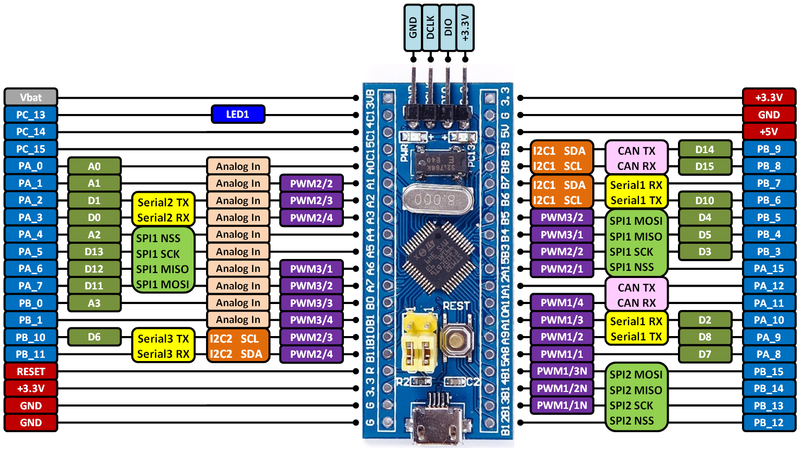
\includegraphics[width=\columnwidth]{stm32/sevenseg/figs/stm_blue}
\end{center}
\caption{Pin Connections of STM-32}
\label{fig:stm_blue}
\end{figure}
\item Make the connections as per the Table \ref{table:USB-UART_connections}
\begin{table}[!h]
\centering
%%%%%%%%%%%%%%%%%%%%%%%%%%%%%%%%%%%%%%%%%%%%%%%%%%%%%%%%%%%%%%%%%%%%%%
%%                                                                  %%
%%  This is the header of a LaTeX2e file exported from Gnumeric.    %%
%%                                                                  %%
%%  This file can be compiled as it stands or included in another   %%
%%  LaTeX document. The table is based on the longtable package so  %%
%%  the longtable options (headers, footers...) can be set in the   %%
%%  preamble section below (see PRAMBLE).                           %%
%%                                                                  %%
%%  To include the file in another, the following two lines must be %%
%%  in the including file:                                          %%
%%        \def\inputGnumericTable{}                                 %%
%%  at the beginning of the file and:                               %%
%%        \input{name-of-this-file.tex}                             %%
%%  where the table is to be placed. Note also that the including   %%
%%  file must use the following packages for the table to be        %%
%%  rendered correctly:                                             %%
%%    \usepackage[latin1]{inputenc}                                 %%
%%    \usepackage{color}                                            %%
%%    \usepackage{array}                                            %%
%%    \usepackage{longtable}                                        %%
%%    \usepackage{calc}                                             %%
%%    \usepackage{multirow}                                         %%
%%    \usepackage{hhline}                                           %%
%%    \usepackage{ifthen}                                           %%
%%  optionally (for landscape tables embedded in another document): %%
%%    \usepackage{lscape}                                           %%
%%                                                                  %%
%%%%%%%%%%%%%%%%%%%%%%%%%%%%%%%%%%%%%%%%%%%%%%%%%%%%%%%%%%%%%%%%%%%%%%



%%  This section checks if we are begin input into another file or  %%
%%  the file will be compiled alone. First use a macro taken from   %%
%%  the TeXbook ex 7.7 (suggestion of Han-Wen Nienhuys).            %%
\def\ifundefined#1{\expandafter\ifx\csname#1\endcsname\relax}


%%  Check for the \def token for inputed files. If it is not        %%
%%  defined, the file will be processed as a standalone and the     %%
%%  preamble will be used.                                          %%
\ifundefined{inputGnumericTable}

%%  We must be able to close or not the document at the end.        %%
	\def\gnumericTableEnd{\end{document}}


%%%%%%%%%%%%%%%%%%%%%%%%%%%%%%%%%%%%%%%%%%%%%%%%%%%%%%%%%%%%%%%%%%%%%%
%%                                                                  %%
%%  This is the PREAMBLE. Change these values to get the right      %%
%%  paper size and other niceties.                                  %%
%%                                                                  %%
%%%%%%%%%%%%%%%%%%%%%%%%%%%%%%%%%%%%%%%%%%%%%%%%%%%%%%%%%%%%%%%%%%%%%%

	\documentclass[12pt%
			  %,landscape%
                    ]{report}
       \usepackage[latin1]{inputenc}
       \usepackage{fullpage}
       \usepackage{color}
       \usepackage{array}
       \usepackage{longtable}
       \usepackage{calc}
       \usepackage{multirow}
       \usepackage{hhline}
       \usepackage{ifthen}

	\begin{document}


%%  End of the preamble for the standalone. The next section is for %%
%%  documents which are included into other LaTeX2e files.          %%
\else

%%  We are not a stand alone document. For a regular table, we will %%
%%  have no preamble and only define the closing to mean nothing.   %%
    \def\gnumericTableEnd{}

%%  If we want landscape mode in an embedded document, comment out  %%
%%  the line above and uncomment the two below. The table will      %%
%%  begin on a new page and run in landscape mode.                  %%
%       \def\gnumericTableEnd{\end{landscape}}
%       \begin{landscape}


%%  End f the else clause for this file being \input.              %%
\fi

%%%%%%%%%%%%%%%%%%%%%%%%%%%%%%%%%%%%%%%%%%%%%%%%%%%%%%%%%%%%%%%%%%%%%%
%%                                                                  %%
%%  The rest is the gnumeric table, except for the closing          %%
%%  statement. Changes below will alter the table's appearance.     %%
%%                                                                  %%
%%%%%%%%%%%%%%%%%%%%%%%%%%%%%%%%%%%%%%%%%%%%%%%%%%%%%%%%%%%%%%%%%%%%%%

\providecommand{\gnumericmathit}[1]{#1} 
%%  Uncomment the next line if you would like your numbers to be in %%
%%  italics if they are italizised in the gnumeric table.           %%
%\renewcommand{\gnumericmathit}[1]{\mathit{#1}}
\providecommand{\gnumericPB}[1]%
{\let\gnumericTemp=\\#1\let\\=\gnumericTemp\hspace{0pt}}
 \ifundefined{gnumericTableWidthDefined}
        \newlength{\gnumericTableWidth}
        \newlength{\gnumericTableWidthComplete}
        \newlength{\gnumericMultiRowLength}
        \global\def\gnumericTableWidthDefined{}
 \fi
%% The following setting protects this code from babel shorthands.  %%
 \ifthenelse{\isundefined{\languageshorthands}}{}{\languageshorthands{english}}
%%  The default table format retains the relative column widths of  %%
%%  gnumeric. They can easily be changed to c, r or l. In that case %%
%%  you may want to comment out the next line and uncomment the one %%
%%  thereafter                                                      %%
\providecommand\gnumbox{\makebox[0pt]}
%%\providecommand\gnumbox[1][]{\makebox}

%% to adjust positions in multirow situations                       %%
\setlength{\bigstrutjot}{\jot}
\setlength{\extrarowheight}{\doublerulesep}

%%  The \setlongtables command keeps column widths the same across  %%
%%  pages. Simply comment out next line for varying column widths.  %%
\setlongtables

\setlength\gnumericTableWidth{%
	98pt+%
	118pt+%
0pt}
\def\gumericNumCols{2}
\setlength\gnumericTableWidthComplete{\gnumericTableWidth+%
         \tabcolsep*\gumericNumCols*2+\arrayrulewidth*\gumericNumCols}
\ifthenelse{\lengthtest{\gnumericTableWidthComplete > \linewidth}}%
         {\def\gnumericScale{1*\ratio{\linewidth-%
                        \tabcolsep*\gumericNumCols*2-%
                        \arrayrulewidth*\gumericNumCols}%
{\gnumericTableWidth}}}%
{\def\gnumericScale{1}}

%%%%%%%%%%%%%%%%%%%%%%%%%%%%%%%%%%%%%%%%%%%%%%%%%%%%%%%%%%%%%%%%%%%%%%
%%                                                                  %%
%% The following are the widths of the various columns. We are      %%
%% defining them here because then they are easier to change.       %%
%% Depending on the cell formats we may use them more than once.    %%
%%                                                                  %%
%%%%%%%%%%%%%%%%%%%%%%%%%%%%%%%%%%%%%%%%%%%%%%%%%%%%%%%%%%%%%%%%%%%%%%

\ifthenelse{\isundefined{\gnumericColA}}{\newlength{\gnumericColA}}{}\settowidth{\gnumericColA}{\begin{tabular}{@{}p{98pt*\gnumericScale}@{}}x\end{tabular}}
\ifthenelse{\isundefined{\gnumericColB}}{\newlength{\gnumericColB}}{}\settowidth{\gnumericColB}{\begin{tabular}{@{}p{118pt*\gnumericScale}@{}}x\end{tabular}}

\begin{tabular}[c]{%
	b{\gnumericColA}%
	b{\gnumericColB}%
	}

%%%%%%%%%%%%%%%%%%%%%%%%%%%%%%%%%%%%%%%%%%%%%%%%%%%%%%%%%%%%%%%%%%%%%%
%%  The tabular options. (Caption, headers... see Goosens, p.124) %%
%	\caption{The Table Caption.}             \\	%
% \hline	% Across the top of the table.
%%  The rest of these options are table rows which are placed on    %%
%%  the first, last or every page. Use \multicolumn if you want.    %%

%%  Header for the first page.                                      %%
%	\multicolumn{2}{c}{The First Header} \\ \hline 
%	\multicolumn{1}{c}{colTag}	%Column 1
%	&\multicolumn{1}{c}{colTag}	\\ \hline %Last column
%	\endfirsthead

%%  The running header definition.                                  %%
%	\hline
%	\multicolumn{2}{l}{\ldots\small\slshape continued} \\ \hline
%	\multicolumn{1}{c}{colTag}	%Column 1
%	&\multicolumn{1}{c}{colTag}	\\ \hline %Last column
%	\endhead

%%  The running footer definition.                                  %%
%	\hline
%	\multicolumn{2}{r}{\small\slshape continued\ldots} \\
%	\endfoot

%%  The ending footer definition.                                   %%
%	\multicolumn{2}{c}{That's all folks} \\ \hline 
%	\endlastfoot
%%%%%%%%%%%%%%%%%%%%%%%%%%%%%%%%%%%%%%%%%%%%%%%%%%%%%%%%%%%%%%%%%%%%%%

\hhline{|-|-}
	 \multicolumn{1}{|p{\gnumericColA}|}%
	{\gnumericPB{\centering}\gnumbox{{\color[rgb]{0.79,0.13,0.12} STM32F103C8 PINS}}}
	&\multicolumn{1}{p{\gnumericColB}|}%
	{\gnumericPB{\centering}\gnumbox{{\color[rgb]{0.79,0.13,0.12} USB2UART PINS}}}
\\
\hhline{|--|}
	 \multicolumn{1}{|p{\gnumericColA}|}%
	{\gnumericPB{\centering}\gnumbox{3.3}}
	&\multicolumn{1}{p{\gnumericColB}|}%
	{\gnumericPB{\centering}\gnumbox{3.3}}
\\
\hhline{|--|}
	 \multicolumn{1}{|p{\gnumericColA}|}%
	{\gnumericPB{\centering}\gnumbox{GND}}
	&\multicolumn{1}{p{\gnumericColB}|}%
	{\gnumericPB{\centering}\gnumbox{GND}}
\\
\hhline{|--|}
	 \multicolumn{1}{|p{\gnumericColA}|}%
	{\gnumericPB{\centering}\gnumbox{A9(TXD)}}
	&\multicolumn{1}{p{\gnumericColB}|}%
	{\gnumericPB{\centering}\gnumbox{RXD}}
\\
\hhline{|--|}
	 \multicolumn{1}{|p{\gnumericColA}|}%
	{\gnumericPB{\centering}\gnumbox{A10(RXD)}}
	&\multicolumn{1}{p{\gnumericColB}|}%
	{\gnumericPB{\centering}\gnumbox{TXD}}
\\
\hhline{|-|-|}
\end{tabular}

\ifthenelse{\isundefined{\languageshorthands}}{}{\languageshorthands{\languagename}}
\gnumericTableEnd

\caption{STM32 to USB-UART connections}
\label{table:USB-UART_connections}
\end{table}
\item Basic onchip led blink program is available at 
\begin{lstlisting}
stm32/ide/setup/codes/src/blink.c
\end{lstlisting}
\item Make sure that platformio.ini file has the following lines
\begin{lstlisting}
[env:bluepill_f103c8]
platform = ststm32
framework = arduino
board = bluepill_f103c8
\end{lstlisting}
\item Now, complile the blink program
\begin{lstlisting}
cd stm32/ide/setup/codes
pio run
\end{lstlisting}
\item With this .bin file will be generated and all the necessary packages will be installed.
\item Before flashing, make sure that STM32 board is in Programming mode
\item See how to enable programming mode in \figref{fig:programming_mode}. This configuration will ensure that the microcontroller enters the system memory programmer on reset.
\begin{figure}[!htb]
\begin{center}
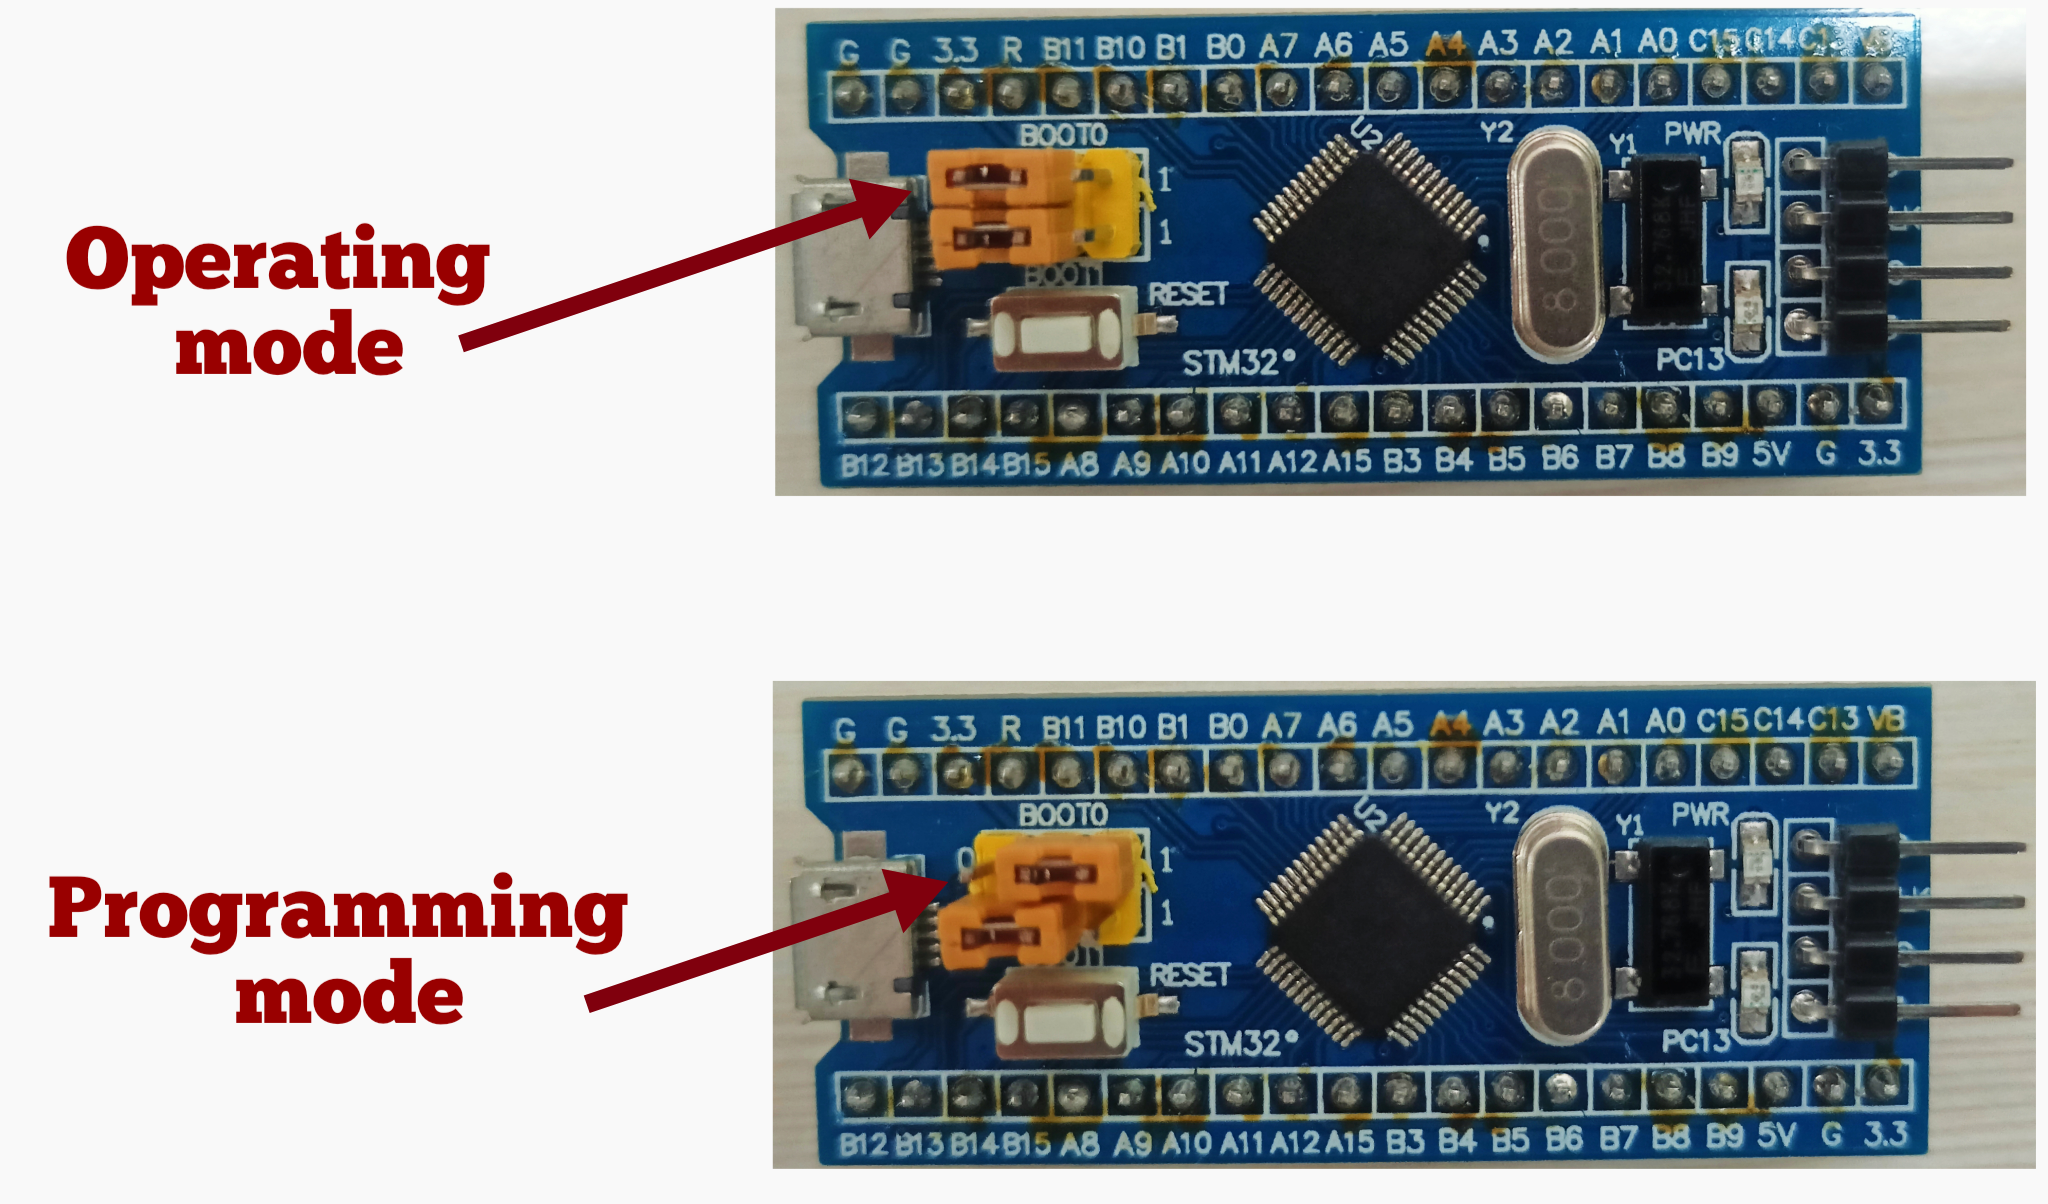
\includegraphics[width=\columnwidth]{stm32/ide/setup/figs/programming_mode.png}
\end{center}
\caption{STM32 Operating and Programming mode}
\label{fig:programming_mode}
\end{figure}
\item After executing 
\begin{lstlisting}
Install STM32-Utils app from playstore
Give the necessary permissions
Connect the USB-UART to OTG
Upload the .bin file to the STM32 board
\end{lstlisting}
\item The inbuilt LED present on the STM32F103C8T6 will start blinking.
\item Change the STM32 board to operating mode as shown in Fig \ref{fig:programming_mode} in order to run your code from the main flash memory.
\end{enumerate}



\newpage
\section{STM32-GCC}
\subsection{Embedded C}
\begin{enumerate}[label=\arabic*.,ref=\theenumi]
%\begin{enumerate}[label=\thesubsection.\arabic*.,ref=\thesubsection.\theenumi]
	\item Copy your codes directory to the termux-debian root directory.
		\begin{lstlisting}
cp -r STM32F103C8T6 ~/STM32F103C8T6/
cd ~/STM32F103C8T6 
make bin
\end{lstlisting}
\item This will generate main.bin.  Flash it using the android app or platformio.
\item Modify main.c in the STM32F103C8T6 directory and modify the code to keep the LED on. Flash it to the STM32 and verify.
\end{enumerate}



\subsection{Seven Segment Display}
\begin{enumerate}[label=\arabic*.,ref=\theenumi]
%\begin{enumerate}[label=\thesubsection.\arabic*.,ref=\thesubsection.\theenumi]
%
\item Make the pin connections in Table \ref{table:stm_ssd} using Figs. \ref{fig:sevenseg} and \ref{fig:stm_blue}.
	
%
\begin{table}[!htb]
\begin{center}
%%%%%%%%%%%%%%%%%%%%%%%%%%%%%%%%%%%%%%%%%%%%%%%%%%%%%%%%%%%%%%%%%%%%%%
%%                                                                  %%
%%  This is the header of a LaTeX2e file exported from Gnumeric.    %%
%%                                                                  %%
%%  This file can be compiled as it stands or included in another   %%
%%  LaTeX document. The table is based on the longtable package so  %%
%%  the longtable options (headers, footers...) can be set in the   %%
%%  preamble section below (see PRAMBLE).                           %%
%%                                                                  %%
%%  To include the file in another, the following two lines must be %%
%%  in the including file:                                          %%
%%        \def\inputGnumericTable{}                                 %%
%%  at the beginning of the file and:                               %%
%%        \input{name-of-this-file.tex}                             %%
%%  where the table is to be placed. Note also that the including   %%
%%  file must use the following packages for the table to be        %%
%%  rendered correctly:                                             %%
%%    \usepackage[latin1]{inputenc}                                 %%
%%    \usepackage{color}                                            %%
%%    \usepackage{array}                                            %%
%%    \usepackage{longtable}                                        %%
%%    \usepackage{calc}                                             %%
%%    \usepackage{multirow}                                         %%
%%    \usepackage{hhline}                                           %%
%%    \usepackage{ifthen}                                           %%
%%  optionally (for landscape tables embedded in another document): %%
%%    \usepackage{lscape}                                           %%
%%                                                                  %%
%%%%%%%%%%%%%%%%%%%%%%%%%%%%%%%%%%%%%%%%%%%%%%%%%%%%%%%%%%%%%%%%%%%%%%



%%  This section checks if we are begin input into another file or  %%
%%  the file will be compiled alone. First use a macro taken from   %%
%%  the TeXbook ex 7.7 (suggestion of Han-Wen Nienhuys).            %%
\def\ifundefined#1{\expandafter\ifx\csname#1\endcsname\relax}


%%  Check for the \def token for inputed files. If it is not        %%
%%  defined, the file will be processed as a standalone and the     %%
%%  preamble will be used.                                          %%
\ifundefined{inputGnumericTable}

%%  We must be able to close or not the document at the end.        %%
	\def\gnumericTableEnd{\end{document}}


%%%%%%%%%%%%%%%%%%%%%%%%%%%%%%%%%%%%%%%%%%%%%%%%%%%%%%%%%%%%%%%%%%%%%%
%%                                                                  %%
%%  This is the PREAMBLE. Change these values to get the right      %%
%%  paper size and other niceties.                                  %%
%%                                                                  %%
%%%%%%%%%%%%%%%%%%%%%%%%%%%%%%%%%%%%%%%%%%%%%%%%%%%%%%%%%%%%%%%%%%%%%%

	\documentclass[12pt%
			  %,landscape%
                    ]{report}
       \usepackage[latin1]{inputenc}
       \usepackage{fullpage}
       \usepackage{color}
       \usepackage{array}
       \usepackage{longtable}
       \usepackage{calc}
       \usepackage{multirow}
       \usepackage{hhline}
       \usepackage{ifthen}

	\begin{document}


%%  End of the preamble for the standalone. The next section is for %%
%%  documents which are included into other LaTeX2e files.          %%
\else

%%  We are not a stand alone document. For a regular table, we will %%
%%  have no preamble and only define the closing to mean nothing.   %%
    \def\gnumericTableEnd{}

%%  If we want landscape mode in an embedded document, comment out  %%
%%  the line above and uncomment the two below. The table will      %%
%%  begin on a new page and run in landscape mode.                  %%
%       \def\gnumericTableEnd{\end{landscape}}
%       \begin{landscape}


%%  End of the else clause for this file being \input.              %%
\fi

%%%%%%%%%%%%%%%%%%%%%%%%%%%%%%%%%%%%%%%%%%%%%%%%%%%%%%%%%%%%%%%%%%%%%%
%%                                                                  %%
%%  The rest is the gnumeric table, except for the closing          %%
%%  statement. Changes below will alter the table's appearance.     %%
%%                                                                  %%
%%%%%%%%%%%%%%%%%%%%%%%%%%%%%%%%%%%%%%%%%%%%%%%%%%%%%%%%%%%%%%%%%%%%%%

\providecommand{\gnumericmathit}[1]{#1} 
%%  Uncomment the next line if you would like your numbers to be in %%
%%  italics if they are italizised in the gnumeric table.           %%
%\renewcommand{\gnumericmathit}[1]{\mathit{#1}}
\providecommand{\gnumericPB}[1]%
{\let\gnumericTemp=\\#1\let\\=\gnumericTemp\hspace{0pt}}
 \ifundefined{gnumericTableWidthDefined}
        \newlength{\gnumericTableWidth}
        \newlength{\gnumericTableWidthComplete}
        \newlength{\gnumericMultiRowLength}
        \global\def\gnumericTableWidthDefined{}
 \fi
%% The following setting protects this code from babel shorthands.  %%
 \ifthenelse{\isundefined{\languageshorthands}}{}{\languageshorthands{english}}
%%  The default table format retains the relative column widths of  %%
%%  gnumeric. They can easily be changed to c, r or l. In that case %%
%%  you may want to comment out the next line and uncomment the one %%
%%  thereafter                                                      %%
\providecommand\gnumbox{\makebox[0pt]}
%%\providecommand\gnumbox[1][]{\makebox}

%% to adjust positions in multirow situations                       %%
\setlength{\bigstrutjot}{\jot}
\setlength{\extrarowheight}{\doublerulesep}

%%  The \setlongtables command keeps column widths the same across  %%
%%  pages. Simply comment out next line for varying column widths.  %%
\setlongtables

\setlength\gnumericTableWidth{%
	53pt+%
	53pt+%
	53pt+%
	53pt+%
	53pt+%
	53pt+%
	53pt+%
	53pt+%
	53pt+%
0pt}
\def\gumericNumCols{9}
\setlength\gnumericTableWidthComplete{\gnumericTableWidth+%
         \tabcolsep*\gumericNumCols*2+\arrayrulewidth*\gumericNumCols}
\ifthenelse{\lengthtest{\gnumericTableWidthComplete > \linewidth}}%
         {\def\gnumericScale{1*\ratio{\linewidth-%
                        \tabcolsep*\gumericNumCols*2-%
                        \arrayrulewidth*\gumericNumCols}%
{\gnumericTableWidth}}}%
{\def\gnumericScale{1}}

%%%%%%%%%%%%%%%%%%%%%%%%%%%%%%%%%%%%%%%%%%%%%%%%%%%%%%%%%%%%%%%%%%%%%%
%%                                                                  %%
%% The following are the widths of the various columns. We are      %%
%% defining them here because then they are easier to change.       %%
%% Depending on the cell formats we may use them more than once.    %%
%%                                                                  %%
%%%%%%%%%%%%%%%%%%%%%%%%%%%%%%%%%%%%%%%%%%%%%%%%%%%%%%%%%%%%%%%%%%%%%%

\ifthenelse{\isundefined{\gnumericColA}}{\newlength{\gnumericColA}}{}\settowidth{\gnumericColA}{\begin{tabular}{@{}p{73pt*\gnumericScale}@{}}x\end{tabular}}
\ifthenelse{\isundefined{\gnumericColB}}{\newlength{\gnumericColB}}{}\settowidth{\gnumericColB}{\begin{tabular}{@{}p{53pt*\gnumericScale}@{}}x\end{tabular}}
\ifthenelse{\isundefined{\gnumericColC}}{\newlength{\gnumericColC}}{}\settowidth{\gnumericColC}{\begin{tabular}{@{}p{53pt*\gnumericScale}@{}}x\end{tabular}}
\ifthenelse{\isundefined{\gnumericColD}}{\newlength{\gnumericColD}}{}\settowidth{\gnumericColD}{\begin{tabular}{@{}p{53pt*\gnumericScale}@{}}x\end{tabular}}
\ifthenelse{\isundefined{\gnumericColE}}{\newlength{\gnumericColE}}{}\settowidth{\gnumericColE}{\begin{tabular}{@{}p{53pt*\gnumericScale}@{}}x\end{tabular}}
\ifthenelse{\isundefined{\gnumericColF}}{\newlength{\gnumericColF}}{}\settowidth{\gnumericColF}{\begin{tabular}{@{}p{53pt*\gnumericScale}@{}}x\end{tabular}}
\ifthenelse{\isundefined{\gnumericColG}}{\newlength{\gnumericColG}}{}\settowidth{\gnumericColG}{\begin{tabular}{@{}p{53pt*\gnumericScale}@{}}x\end{tabular}}
\ifthenelse{\isundefined{\gnumericColH}}{\newlength{\gnumericColH}}{}\settowidth{\gnumericColH}{\begin{tabular}{@{}p{53pt*\gnumericScale}@{}}x\end{tabular}}
\ifthenelse{\isundefined{\gnumericColI}}{\newlength{\gnumericColI}}{}\settowidth{\gnumericColI}{\begin{tabular}{@{}p{33pt*\gnumericScale}@{}}x\end{tabular}}

\begin{longtable}[c]{%
	b{\gnumericColA}%
	b{\gnumericColB}%
	b{\gnumericColC}%
	b{\gnumericColD}%
	b{\gnumericColE}%
	b{\gnumericColF}%
	b{\gnumericColG}%
	b{\gnumericColH}%
	b{\gnumericColI}%
	}

%%%%%%%%%%%%%%%%%%%%%%%%%%%%%%%%%%%%%%%%%%%%%%%%%%%%%%%%%%%%%%%%%%%%%%
%%  The longtable options. (Caption, headers... see Goosens, p.124) %%
%	\caption{The Table Caption.}             \\	%
% \hline	% Across the top of the table.
%%  The rest of these options are table rows which are placed on    %%
%%  the first, last or every page. Use \multicolumn if you want.    %%

%%  Header for the first page.                                      %%
%	\multicolumn{9}{c}{The First Header} \\ \hline 
%	\multicolumn{1}{c}{colTag}	%Column 1
%	&\multicolumn{1}{c}{colTag}	%Column 2
%	&\multicolumn{1}{c}{colTag}	%Column 3
%	&\multicolumn{1}{c}{colTag}	%Column 4
%	&\multicolumn{1}{c}{colTag}	%Column 5
%	&\multicolumn{1}{c}{colTag}	%Column 6
%	&\multicolumn{1}{c}{colTag}	%Column 7
%	&\multicolumn{1}{c}{colTag}	%Column 8
%	&\multicolumn{1}{c}{colTag}	\\ \hline %Last column
%	\endfirsthead

%%  The running header definition.                                  %%
%	\hline
%	\multicolumn{9}{l}{\ldots\small\slshape continued} \\ \hline
%	\multicolumn{1}{c}{colTag}	%Column 1
%	&\multicolumn{1}{c}{colTag}	%Column 2
%	&\multicolumn{1}{c}{colTag}	%Column 3
%	&\multicolumn{1}{c}{colTag}	%Column 4
%	&\multicolumn{1}{c}{colTag}	%Column 5
%	&\multicolumn{1}{c}{colTag}	%Column 6
%	&\multicolumn{1}{c}{colTag}	%Column 7
%	&\multicolumn{1}{c}{colTag}	%Column 8
%	&\multicolumn{1}{c}{colTag}	\\ \hline %Last column
%	\endhead

%%  The running footer definition.                                  %%
%	\hline
%	\multicolumn{9}{r}{\small\slshape continued\ldots} \\
%	\endfoot

%%  The ending footer definition.                                   %%
%	\multicolumn{9}{c}{That's all folks} \\ \hline 
%	\endlastfoot
%%%%%%%%%%%%%%%%%%%%%%%%%%%%%%%%%%%%%%%%%%%%%%%%%%%%%%%%%%%%%%%%%%%%%%

\hhline{|-|-|-|-|-|-|-|-|-}
	 \multicolumn{1}{|p{\gnumericColA}|}%
	{\gnumericPB{\raggedright}\gnumbox[l]{\textbf{STM32}}}
	&\multicolumn{1}{p{\gnumericColB}|}%
	{\gnumericPB{\centering}\gnumbox{\textbf{PB9}}}
	&\multicolumn{1}{p{\gnumericColC}|}%
	{\gnumericPB{\centering}\gnumbox{\textbf{PB8}}}
	&\multicolumn{1}{p{\gnumericColD}|}%
	{\gnumericPB{\centering}\gnumbox{\textbf{PB7}}}
	&\multicolumn{1}{p{\gnumericColE}|}%
	{\gnumericPB{\centering}\gnumbox{\textbf{PB6}}}
	&\multicolumn{1}{p{\gnumericColF}|}%
	{\gnumericPB{\centering}\gnumbox{\textbf{PB5}}}
	&\multicolumn{1}{p{\gnumericColG}|}%
	{\gnumericPB{\centering}\gnumbox{\textbf{PB4}}}
	&\multicolumn{1}{p{\gnumericColH}|}%
	{\gnumericPB{\centering}\gnumbox{\textbf{PB3}}}
	&\multicolumn{1}{p{\gnumericColI}|}%
	{\gnumericPB{\centering}\gnumbox{\textbf{3.3V}}}
\\
\hhline{|---------|}
	 \multicolumn{1}{|p{\gnumericColA}|}%
	{\gnumericPB{\raggedright}\gnumbox[l]{\textbf{DISPLAY}}}
	&\multicolumn{1}{p{\gnumericColB}|}%
	{\gnumericPB{\centering}\gnumbox{\textbf{a}}}
	&\multicolumn{1}{p{\gnumericColC}|}%
	{\gnumericPB{\centering}\gnumbox{\textbf{b}}}
	&\multicolumn{1}{p{\gnumericColD}|}%
	{\gnumericPB{\centering}\gnumbox{\textbf{c}}}
	&\multicolumn{1}{p{\gnumericColE}|}%
	{\gnumericPB{\centering}\gnumbox{\textbf{d}}}
	&\multicolumn{1}{p{\gnumericColF}|}%
	{\gnumericPB{\centering}\gnumbox{\textbf{e}}}
	&\multicolumn{1}{p{\gnumericColG}|}%
	{\gnumericPB{\centering}\gnumbox{\textbf{f}}}
	&\multicolumn{1}{p{\gnumericColH}|}%
	{\gnumericPB{\centering}\gnumbox{\textbf{g}}}
	&\multicolumn{1}{p{\gnumericColI}|}%
	{\gnumericPB{\centering}\gnumbox{\textbf{COM}}}
\\
\hhline{|---------|}
	 \multicolumn{1}{|p{\gnumericColA}|}%
	{\gnumericPB{\centering}\gnumbox{\textbf{0}}}
	&\multicolumn{1}{p{\gnumericColB}|}%
	{\gnumericPB{\centering}\gnumbox{0}}
	&\multicolumn{1}{p{\gnumericColC}|}%
	{\gnumericPB{\centering}\gnumbox{0}}
	&\multicolumn{1}{p{\gnumericColD}|}%
	{\gnumericPB{\centering}\gnumbox{0}}
	&\multicolumn{1}{p{\gnumericColE}|}%
	{\gnumericPB{\centering}\gnumbox{0}}
	&\multicolumn{1}{p{\gnumericColF}|}%
	{\gnumericPB{\centering}\gnumbox{0}}
	&\multicolumn{1}{p{\gnumericColG}|}%
	{\gnumericPB{\centering}\gnumbox{0}}
	&\multicolumn{1}{p{\gnumericColH}|}%
	{\gnumericPB{\centering}\gnumbox{1}}
	&\multicolumn{1}{p{\gnumericColI}|}%
	{}
\\
\hhline{|---------|}
	 \multicolumn{1}{|p{\gnumericColA}|}%
	{\gnumericPB{\centering}\gnumbox{\textbf{1}}}
	&\multicolumn{1}{p{\gnumericColB}|}%
	{\gnumericPB{\centering}\gnumbox{1}}
	&\multicolumn{1}{p{\gnumericColC}|}%
	{\gnumericPB{\centering}\gnumbox{0}}
	&\multicolumn{1}{p{\gnumericColD}|}%
	{\gnumericPB{\centering}\gnumbox{0}}
	&\multicolumn{1}{p{\gnumericColE}|}%
	{\gnumericPB{\centering}\gnumbox{1}}
	&\multicolumn{1}{p{\gnumericColF}|}%
	{\gnumericPB{\centering}\gnumbox{1}}
	&\multicolumn{1}{p{\gnumericColG}|}%
	{\gnumericPB{\centering}\gnumbox{1}}
	&\multicolumn{1}{p{\gnumericColH}|}%
	{\gnumericPB{\centering}\gnumbox{1}}
	&\multicolumn{1}{p{\gnumericColI}|}%
	{}
\\
\hhline{|---------|}
	 \multicolumn{1}{|p{\gnumericColA}|}%
	{\gnumericPB{\centering}\gnumbox{\textbf{2}}}
	&\multicolumn{1}{p{\gnumericColB}|}%
	{\gnumericPB{\centering}\gnumbox{0}}
	&\multicolumn{1}{p{\gnumericColC}|}%
	{\gnumericPB{\centering}\gnumbox{0}}
	&\multicolumn{1}{p{\gnumericColD}|}%
	{\gnumericPB{\centering}\gnumbox{1}}
	&\multicolumn{1}{p{\gnumericColE}|}%
	{\gnumericPB{\centering}\gnumbox{0}}
	&\multicolumn{1}{p{\gnumericColF}|}%
	{\gnumericPB{\centering}\gnumbox{0}}
	&\multicolumn{1}{p{\gnumericColG}|}%
	{\gnumericPB{\centering}\gnumbox{1}}
	&\multicolumn{1}{p{\gnumericColH}|}%
	{\gnumericPB{\centering}\gnumbox{0}}
	&\multicolumn{1}{p{\gnumericColI}|}%
	{}
\\
\hhline{|---------|}
	 \multicolumn{1}{|p{\gnumericColA}|}%
	{\gnumericPB{\centering}\gnumbox{\textbf{3}}}
	&\multicolumn{1}{p{\gnumericColB}|}%
	{\gnumericPB{\centering}\gnumbox{0}}
	&\multicolumn{1}{p{\gnumericColC}|}%
	{\gnumericPB{\centering}\gnumbox{0}}
	&\multicolumn{1}{p{\gnumericColD}|}%
	{\gnumericPB{\centering}\gnumbox{0}}
	&\multicolumn{1}{p{\gnumericColE}|}%
	{\gnumericPB{\centering}\gnumbox{0}}
	&\multicolumn{1}{p{\gnumericColF}|}%
	{\gnumericPB{\centering}\gnumbox{1}}
	&\multicolumn{1}{p{\gnumericColG}|}%
	{\gnumericPB{\centering}\gnumbox{1}}
	&\multicolumn{1}{p{\gnumericColH}|}%
	{\gnumericPB{\centering}\gnumbox{0}}
	&\multicolumn{1}{p{\gnumericColI}|}%
	{}
\\
\hhline{|---------|}
	 \multicolumn{1}{|p{\gnumericColA}|}%
	{\gnumericPB{\centering}\gnumbox{\textbf{4}}}
	&\multicolumn{1}{p{\gnumericColB}|}%
	{\gnumericPB{\centering}\gnumbox{1}}
	&\multicolumn{1}{p{\gnumericColC}|}%
	{\gnumericPB{\centering}\gnumbox{0}}
	&\multicolumn{1}{p{\gnumericColD}|}%
	{\gnumericPB{\centering}\gnumbox{0}}
	&\multicolumn{1}{p{\gnumericColE}|}%
	{\gnumericPB{\centering}\gnumbox{1}}
	&\multicolumn{1}{p{\gnumericColF}|}%
	{\gnumericPB{\centering}\gnumbox{1}}
	&\multicolumn{1}{p{\gnumericColG}|}%
	{\gnumericPB{\centering}\gnumbox{0}}
	&\multicolumn{1}{p{\gnumericColH}|}%
	{\gnumericPB{\centering}\gnumbox{0}}
	&\multicolumn{1}{p{\gnumericColI}|}%
	{}
\\
\hhline{|---------|}
	 \multicolumn{1}{|p{\gnumericColA}|}%
	{\gnumericPB{\centering}\gnumbox{\textbf{5}}}
	&\multicolumn{1}{p{\gnumericColB}|}%
	{\gnumericPB{\centering}\gnumbox{0}}
	&\multicolumn{1}{p{\gnumericColC}|}%
	{\gnumericPB{\centering}\gnumbox{1}}
	&\multicolumn{1}{p{\gnumericColD}|}%
	{\gnumericPB{\centering}\gnumbox{0}}
	&\multicolumn{1}{p{\gnumericColE}|}%
	{\gnumericPB{\centering}\gnumbox{0}}
	&\multicolumn{1}{p{\gnumericColF}|}%
	{\gnumericPB{\centering}\gnumbox{1}}
	&\multicolumn{1}{p{\gnumericColG}|}%
	{\gnumericPB{\centering}\gnumbox{0}}
	&\multicolumn{1}{p{\gnumericColH}|}%
	{\gnumericPB{\centering}\gnumbox{0}}
	&\multicolumn{1}{p{\gnumericColI}|}%
	{}
\\
\hhline{|---------|}
	 \multicolumn{1}{|p{\gnumericColA}|}%
	{\gnumericPB{\centering}\gnumbox{\textbf{6}}}
	&\multicolumn{1}{p{\gnumericColB}|}%
	{\gnumericPB{\centering}\gnumbox{0}}
	&\multicolumn{1}{p{\gnumericColC}|}%
	{\gnumericPB{\centering}\gnumbox{1}}
	&\multicolumn{1}{p{\gnumericColD}|}%
	{\gnumericPB{\centering}\gnumbox{0}}
	&\multicolumn{1}{p{\gnumericColE}|}%
	{\gnumericPB{\centering}\gnumbox{0}}
	&\multicolumn{1}{p{\gnumericColF}|}%
	{\gnumericPB{\centering}\gnumbox{0}}
	&\multicolumn{1}{p{\gnumericColG}|}%
	{\gnumericPB{\centering}\gnumbox{0}}
	&\multicolumn{1}{p{\gnumericColH}|}%
	{\gnumericPB{\centering}\gnumbox{0}}
	&\multicolumn{1}{p{\gnumericColI}|}%
	{}
\\
\hhline{|---------|}
	 \multicolumn{1}{|p{\gnumericColA}|}%
	{\gnumericPB{\centering}\gnumbox{\textbf{7}}}
	&\multicolumn{1}{p{\gnumericColB}|}%
	{\gnumericPB{\centering}\gnumbox{0}}
	&\multicolumn{1}{p{\gnumericColC}|}%
	{\gnumericPB{\centering}\gnumbox{0}}
	&\multicolumn{1}{p{\gnumericColD}|}%
	{\gnumericPB{\centering}\gnumbox{0}}
	&\multicolumn{1}{p{\gnumericColE}|}%
	{\gnumericPB{\centering}\gnumbox{1}}
	&\multicolumn{1}{p{\gnumericColF}|}%
	{\gnumericPB{\centering}\gnumbox{1}}
	&\multicolumn{1}{p{\gnumericColG}|}%
	{\gnumericPB{\centering}\gnumbox{1}}
	&\multicolumn{1}{p{\gnumericColH}|}%
	{\gnumericPB{\centering}\gnumbox{1}}
	&\multicolumn{1}{p{\gnumericColI}|}%
	{}
\\
\hhline{|---------|}
	 \multicolumn{1}{|p{\gnumericColA}|}%
	{\gnumericPB{\centering}\gnumbox{\textbf{8}}}
	&\multicolumn{1}{p{\gnumericColB}|}%
	{\gnumericPB{\centering}\gnumbox{0}}
	&\multicolumn{1}{p{\gnumericColC}|}%
	{\gnumericPB{\centering}\gnumbox{0}}
	&\multicolumn{1}{p{\gnumericColD}|}%
	{\gnumericPB{\centering}\gnumbox{0}}
	&\multicolumn{1}{p{\gnumericColE}|}%
	{\gnumericPB{\centering}\gnumbox{0}}
	&\multicolumn{1}{p{\gnumericColF}|}%
	{\gnumericPB{\centering}\gnumbox{0}}
	&\multicolumn{1}{p{\gnumericColG}|}%
	{\gnumericPB{\centering}\gnumbox{0}}
	&\multicolumn{1}{p{\gnumericColH}|}%
	{\gnumericPB{\centering}\gnumbox{0}}
	&\multicolumn{1}{p{\gnumericColI}|}%
	{}
\\
\hhline{|---------|}
	 \multicolumn{1}{|p{\gnumericColA}|}%
	{\gnumericPB{\centering}\gnumbox{\textbf{9}}}
	&\multicolumn{1}{p{\gnumericColB}|}%
	{\gnumericPB{\centering}\gnumbox{0}}
	&\multicolumn{1}{p{\gnumericColC}|}%
	{\gnumericPB{\centering}\gnumbox{0}}
	&\multicolumn{1}{p{\gnumericColD}|}%
	{\gnumericPB{\centering}\gnumbox{0}}
	&\multicolumn{1}{p{\gnumericColE}|}%
	{\gnumericPB{\centering}\gnumbox{0}}
	&\multicolumn{1}{p{\gnumericColF}|}%
	{\gnumericPB{\centering}\gnumbox{1}}
	&\multicolumn{1}{p{\gnumericColG}|}%
	{\gnumericPB{\centering}\gnumbox{0}}
	&\multicolumn{1}{p{\gnumericColH}|}%
	{\gnumericPB{\centering}\gnumbox{0}}
	&\multicolumn{1}{p{\gnumericColI}|}%
	{}
\\
\hhline{|-|-|-|-|-|-|-|-|-|}
\end{longtable}

\ifthenelse{\isundefined{\languageshorthands}}{}{\languageshorthands{\languagename}}
\gnumericTableEnd

\end{center}
\caption{STM-32 and Seven Segment Display Connections}
\label{table:stm_ssd}
\end{table}
%
\item Execute the following code 
\begin{lstlisting}
stm32/sevenseg/codes/sevenseg_example.c
\end{lstlisting}

%\begin{problem}
%In the STM32F103C8T6 directory,
%\begin{lstlisting}
%cp sevenseg.c main.c
%\end{lstlisting}
%Generate the number 0 by executing \textbf{main.c} and flashing to the STM32. 
%\end{problem}	
%
\item Explain the process of generating the number 0 using the following instruction.
\begin{lstlisting}
GPIOB->ODR = 0xFC08;
\end{lstlisting}
\solution ODR is the Output Data Register, which is used to write outputs to the GPIO pins. The 16 bit number 0xFC08 on the RHS represents the pin configuration for the pins of port B of STM32F103C8T6, which are numbered PB15-PB0 in that order.  See Table \ref{table:stm_ssd}.
\item Repeat the above exercise to generate the numbers 1-9 on the display.
\item The previous instructions set the bits in the unused ports PB15-PB10 and PB2-PB0. This may be undesirable in some cases. Generate 0 by not disturbing 
the unused pins.
\\
\solution The following instructions help accomplish this. The first instruction resets PB4-PB9.  The second instruction sets the PB3 pin. The other pins are
undisturbed.
\begin{lstlisting}
GPIOB->BRR = (1<<4)|(1<<5)|(1<<6)|(1<<7)|(1<<8)|(1<<9); // (Led ON)		
GPIOB->BSRR = (1<<3); // (Led OFF)					
\end{lstlisting}
%\section{Manual Display Control}
%\input{./chapters/chapter1}
%
\item Write a program to take a 4-bit BCD as input from hardware (GND or VDD) and show the next number on the seven segment display.
\\
\solution The following program takes 4 bits as input from pins PB12-PB15 and displays the output on a seven segment display. The next number
can be displayed by slightly modifying the code.
\begin{lstlisting}
stm32/sevenseg/codes/bin2dec_example.c
\end{lstlisting}
\end{enumerate}


\subsection{GPIO Output}
\begin{enumerate}[label=\arabic*.,ref=\theenumi]
%\begin{enumerate}[label=\thesubsection.\arabic*.,ref=\thesubsection.\theenumi]
\item Connect the USB-UART to STM32.   The hardware connections between the USB-UART, STM32 and LED are available in Table \ref{table:/gpio/pins}. Make sure that the LED is connected to PB4 through the resistor.
\begin{table}[!ht]
\centering
%%%%%%%%%%%%%%%%%%%%%%%%%%%%%%%%%%%%%%%%%%%%%%%%%%%%%%%%%%%%%%%%%%%%%%
%%                                                                  %%
%%  This is the header of a LaTeX2e file exported from Gnumeric.    %%
%%                                                                  %%
%%  This file can be compiled as it stands or included in another   %%
%%  LaTeX document. The table is based on the longtable package so  %%
%%  the longtable options (headers, footers...) can be set in the   %%
%%  preamble section below (see PRAMBLE).                           %%
%%                                                                  %%
%%  To include the file in another, the following two lines must be %%
%%  in the including file:                                          %%
%%        \def\inputGnumericTable{}                                 %%
%%  at the beginning of the file and:                               %%
%%        \input{name-of-this-file.tex}                             %%
%%  where the table is to be placed. Note also that the including   %%
%%  file must use the following packages for the table to be        %%
%%  rendered correctly:                                             %%
%%    \usepackage[latin1]{inputenc}                                 %%
%%    \usepackage{color}                                            %%
%%    \usepackage{array}                                            %%
%%    \usepackage{longtable}                                        %%
%%    \usepackage{calc}                                             %%
%%    \usepackage{multirow}                                         %%
%%    \usepackage{hhline}                                           %%
%%    \usepackage{ifthen}                                           %%
%%  optionally (for landscape tables embedded in another document): %%
%%    \usepackage{lscape}                                           %%
%%                                                                  %%
%%%%%%%%%%%%%%%%%%%%%%%%%%%%%%%%%%%%%%%%%%%%%%%%%%%%%%%%%%%%%%%%%%%%%%



%%  This section checks if we are begin input into another file or  %%
%%  the file will be compiled alone. First use a macro taken from   %%
%%  the TeXbook ex 7.7 (suggestion of Han-Wen Nienhuys).            %%
\def\ifundefined#1{\expandafter\ifx\csname#1\endcsname\relax}


%%  Check for the \def token for inputed files. If it is not        %%
%%  defined, the file will be processed as a standalone and the     %%
%%  preamble will be used.                                          %%
\ifundefined{inputGnumericTable}

%%  We must be able to close or not the document at the end.        %%
	\def\gnumericTableEnd{\end{document}}


%%%%%%%%%%%%%%%%%%%%%%%%%%%%%%%%%%%%%%%%%%%%%%%%%%%%%%%%%%%%%%%%%%%%%%
%%                                                                  %%
%%  This is the PREAMBLE. Change these values to get the right      %%
%%  paper size and other niceties.                                  %%
%%                                                                  %%
%%%%%%%%%%%%%%%%%%%%%%%%%%%%%%%%%%%%%%%%%%%%%%%%%%%%%%%%%%%%%%%%%%%%%%

	\documentclass[12pt%
			  %,landscape%
                    ]{report}
       \usepackage[latin1]{inputenc}
       \usepackage{fullpage}
       \usepackage{color}
       \usepackage{array}
       \usepackage{longtable}
       \usepackage{calc}
       \usepackage{multirow}
       \usepackage{hhline}
       \usepackage{ifthen}

	\begin{document}


%%  End of the preamble for the standalone. The next section is for %%
%%  documents which are included into other LaTeX2e files.          %%
\else

%%  We are not a stand alone document. For a regular table, we will %%
%%  have no preamble and only define the closing to mean nothing.   %%
    \def\gnumericTableEnd{}

%%  If we want landscape mode in an embedded document, comment out  %%
%%  the line above and uncomment the two below. The table will      %%
%%  begin on a new page and run in landscape mode.                  %%
%       \def\gnumericTableEnd{\end{landscape}}
%       \begin{landscape}


%%  End f the else clause for this file being \input.              %%
\fi

%%%%%%%%%%%%%%%%%%%%%%%%%%%%%%%%%%%%%%%%%%%%%%%%%%%%%%%%%%%%%%%%%%%%%%
%%                                                                  %%
%%  The rest is the gnumeric table, except for the closing          %%
%%  statement. Changes below will alter the table's appearance.     %%
%%                                                                  %%
%%%%%%%%%%%%%%%%%%%%%%%%%%%%%%%%%%%%%%%%%%%%%%%%%%%%%%%%%%%%%%%%%%%%%%

\providecommand{\gnumericmathit}[1]{#1} 
%%  Uncomment the next line if you would like your numbers to be in %%
%%  italics if they are italizised in the gnumeric table.           %%
%\renewcommand{\gnumericmathit}[1]{\mathit{#1}}
\providecommand{\gnumericPB}[1]%
{\let\gnumericTemp=\\#1\let\\=\gnumericTemp\hspace{0pt}}
 \ifundefined{gnumericTableWidthDefined}
        \newlength{\gnumericTableWidth}
        \newlength{\gnumericTableWidthComplete}
        \newlength{\gnumericMultiRowLength}
        \global\def\gnumericTableWidthDefined{}
 \fi
%% The following setting protects this code from babel shorthands.  %%
 \ifthenelse{\isundefined{\languageshorthands}}{}{\languageshorthands{english}}
%%  The default table format retains the relative column widths of  %%
%%  gnumeric. They can easily be changed to c, r or l. In that case %%
%%  you may want to comment out the next line and uncomment the one %%
%%  thereafter                                                      %%
\providecommand\gnumbox{\makebox[0pt]}
%%\providecommand\gnumbox[1][]{\makebox}

%% to adjust positions in multirow situations                       %%
\setlength{\bigstrutjot}{\jot}
\setlength{\extrarowheight}{\doublerulesep}

%%  The \setlongtables command keeps column widths the same across  %%
%%  pages. Simply comment out next line for varying column widths.  %%
\setlongtables

\setlength\gnumericTableWidth{%
	40pt+%
	40pt+%
	27pt+%
0pt}
\def\gumericNumCols{3}
\setlength\gnumericTableWidthComplete{\gnumericTableWidth+%
         \tabcolsep*\gumericNumCols*2+\arrayrulewidth*\gumericNumCols}
\ifthenelse{\lengthtest{\gnumericTableWidthComplete > \linewidth}}%
         {\def\gnumericScale{\ratio{\linewidth-%
                        \tabcolsep*\gumericNumCols*2-%
                        \arrayrulewidth*\gumericNumCols}%
{\gnumericTableWidth}}}%
{\def\gnumericScale{1}}

%%%%%%%%%%%%%%%%%%%%%%%%%%%%%%%%%%%%%%%%%%%%%%%%%%%%%%%%%%%%%%%%%%%%%%
%%                                                                  %%
%% The following are the widths of the various columns. We are      %%
%% defining them here because then they are easier to change.       %%
%% Depending on the cell formats we may use them more than once.    %%
%%                                                                  %%
%%%%%%%%%%%%%%%%%%%%%%%%%%%%%%%%%%%%%%%%%%%%%%%%%%%%%%%%%%%%%%%%%%%%%%

\ifthenelse{\isundefined{\gnumericColA}}{\newlength{\gnumericColA}}{}\settowidth{\gnumericColA}{\begin{tabular}{@{}p{40pt*\gnumericScale}@{}}x\end{tabular}}
\ifthenelse{\isundefined{\gnumericColB}}{\newlength{\gnumericColB}}{}\settowidth{\gnumericColB}{\begin{tabular}{@{}p{40pt*\gnumericScale}@{}}x\end{tabular}}
\ifthenelse{\isundefined{\gnumericColC}}{\newlength{\gnumericColC}}{}\settowidth{\gnumericColC}{\begin{tabular}{@{}p{27pt*\gnumericScale}@{}}x\end{tabular}}

\begin{tabular}[c]{%
	b{\gnumericColA}%
	b{\gnumericColB}%
	b{\gnumericColC}%
	}

%%%%%%%%%%%%%%%%%%%%%%%%%%%%%%%%%%%%%%%%%%%%%%%%%%%%%%%%%%%%%%%%%%%%%%
%%  The longtable options. (Caption, headers... see Goosens, p.124) %%
%	\caption{The Table Caption.}             \\	%
% \hline	% Across the top of the table.
%%  The rest of these options are table rows which are placed on    %%
%%  the first, last or every page. Use \multicolumn if you want.    %%

%%  Header for the first page.                                      %%
%	\multicolumn{3}{c}{The First Header} \\ \hline 
%	\multicolumn{1}{c}{colTag}	%Column 1
%	&\multicolumn{1}{c}{colTag}	%Column 2
%	&\multicolumn{1}{c}{colTag}	\\ \hline %Last column
%	\endfirsthead

%%  The running header definition.                                  %%
%	\hline
%	\multicolumn{3}{l}{\ldots\small\slshape continued} \\ \hline
%	\multicolumn{1}{c}{colTag}	%Column 1
%	&\multicolumn{1}{c}{colTag}	%Column 2
%	&\multicolumn{1}{c}{colTag}	\\ \hline %Last column
%	\endhead

%%  The running footer definition.                                  %%
%	\hline
%	\multicolumn{3}{r}{\small\slshape continued\ldots} \\
%	\endfoot

%%  The ending footer definition.                                   %%
%	\multicolumn{3}{c}{That's all folks} \\ \hline 
%	\endlastfoot
%%%%%%%%%%%%%%%%%%%%%%%%%%%%%%%%%%%%%%%%%%%%%%%%%%%%%%%%%%%%%%%%%%%%%%

\hhline{|-|-|-}
	 \multicolumn{1}{|p{\gnumericColA}|}%
	{\gnumericPB{\centering}\gnumbox{\textbf{STM32}}}
	&\multicolumn{1}{p{\gnumericColB}|}%
	{\gnumericPB{\centering}\gnumbox{\textbf{UART}}}
	&\multicolumn{1}{p{\gnumericColC}|}%
	{\gnumericPB{\centering}\gnumbox{\textbf{LED}}}
\\
\hhline{|---|}
	 \multicolumn{1}{|p{\gnumericColA}|}%
	{\gnumericPB{\raggedright}\gnumbox[l]{GND}}
	&\multicolumn{1}{p{\gnumericColB}|}%
	{\gnumericPB{\raggedright}\gnumbox[l]{GND}}
	&\multicolumn{1}{p{\gnumericColC}|}%
	{\gnumericPB{\centering}\gnumbox{-}}
\\
\hhline{|---|}
	 \multicolumn{1}{|p{\gnumericColA}|}%
	{\gnumericPB{\raggedright}\gnumbox[l]{3.3V}}
	&\multicolumn{1}{p{\gnumericColB}|}%
	{\gnumericPB{\raggedright}\gnumbox[l]{3.3V}}
	&\multicolumn{1}{p{\gnumericColC}|}%
	{}
\\
\hhline{|---|}
	 \multicolumn{1}{|p{\gnumericColA}|}%
	{\gnumericPB{\raggedright}\gnumbox[l]{A9(Txd)}}
	&\multicolumn{1}{p{\gnumericColB}|}%
	{\gnumericPB{\raggedright}\gnumbox[l]{Rxd}}
	&\multicolumn{1}{p{\gnumericColC}|}%
	{}
\\
\hhline{|---|}
	 \multicolumn{1}{|p{\gnumericColA}|}%
	{\gnumericPB{\raggedright}\gnumbox[l]{A10(Rxd)}}
	&\multicolumn{1}{p{\gnumericColB}|}%
	{\gnumericPB{\raggedright}\gnumbox[l]{Txd}}
	&\multicolumn{1}{p{\gnumericColC}|}%
	{}
\\
\hhline{|---|}
	 \multicolumn{1}{|p{\gnumericColA}|}%
	{\gnumericPB{\raggedright}\gnumbox[l]{PB4}}
	&\multicolumn{1}{p{\gnumericColB}|}%
	{}
	&\multicolumn{1}{p{\gnumericColC}|}%
	{\gnumericPB{\centering}\gnumbox{+}}
\\
\hhline{|-|-|-|}
\end{tabular}

\ifthenelse{\isundefined{\languageshorthands}}{}{\languageshorthands{\languagename}}
\gnumericTableEnd

\caption{USB-UART to STM32 connections}
\label{table:/gpio/pins}
\end{table}
%
\item Execute 
\begin{lstlisting}
gpio/codes/gpio_example.c
\end{lstlisting}
\item Modify the above program to turn the LED off.
\item Explain the following line.
\begin{lstlisting}
AFIO->MAPR = AFIO_MAPR_SWJ_CFG_JTAGDISABLE;
\end{lstlisting}
\solution By default, the PB3 and PB4 pins in the STM32F103C8T6 board cannot be used as GPIO pins.  The above
command allows these pins to be configured for GPIO.
\item What does the following command do?
\begin{lstlisting}
GPIOB->CRL = 0x00030000;	
\end{lstlisting}
\solution The STM32F103C8T6 has ports A and B, each  having 16 pins that can be used as GPIO output.  The above command enables the pin B4 of port B as an output pin
See Tables \ref{table:gpio_enable}.

\begin{table}[!ht]
\centering
\small
%\resizebox{\textwidth}{!}{
%%%%%%%%%%%%%%%%%%%%%%%%%%%%%%%%%%%%%%%%%%%%%%%%%%%%%%%%%%%%%%%%%%%%%%
%%                                                                  %%
%%  This is the header of a LaTeX2e file exported from Gnumeric.    %%
%%                                                                  %%
%%  This file can be compiled as it stands or included in another   %%
%%  LaTeX document. The table is based on the longtable package so  %%
%%  the longtable options (headers, footers...) can be set in the   %%
%%  preamble section below (see PRAMBLE).                           %%
%%                                                                  %%
%%  To include the file in another, the following two lines must be %%
%%  in the including file:                                          %%
%%        \def\inputGnumericTable{}                                 %%
%%  at the beginning of the file and:                               %%
%%        \input{name-of-this-file.tex}                             %%
%%  where the table is to be placed. Note also that the including   %%
%%  file must use the following packages for the table to be        %%
%%  rendered correctly:                                             %%
%%    \usepackage[latin1]{inputenc}                                 %%
%%    \usepackage{color}                                            %%
%%    \usepackage{array}                                            %%
%%    \usepackage{longtable}                                        %%
%%    \usepackage{calc}                                             %%
%%    \usepackage{multirow}                                         %%
%%    \usepackage{hhline}                                           %%
%%    \usepackage{ifthen}                                           %%
%%  optionally (for landscape tables embedded in another document): %%
%%    \usepackage{lscape}                                           %%
%%                                                                  %%
%%%%%%%%%%%%%%%%%%%%%%%%%%%%%%%%%%%%%%%%%%%%%%%%%%%%%%%%%%%%%%%%%%%%%%



%%  This section checks if we are begin input into another file or  %%
%%  the file will be compiled alone. First use a macro taken from   %%
%%  the TeXbook ex 7.7 (suggestion of Han-Wen Nienhuys).            %%
\def\ifundefined#1{\expandafter\ifx\csname#1\endcsname\relax}


%%  Check for the \def token for inputed files. If it is not        %%
%%  defined, the file will be processed as a standalone and the     %%
%%  preamble will be used.                                          %%
\ifundefined{inputGnumericTable}

%%  We must be able to close or not the document at the end.        %%
	\def\gnumericTableEnd{\end{document}}


%%%%%%%%%%%%%%%%%%%%%%%%%%%%%%%%%%%%%%%%%%%%%%%%%%%%%%%%%%%%%%%%%%%%%%
%%                                                                  %%
%%  This is the PREAMBLE. Change these values to get the right      %%
%%  paper size and other niceties.                                  %%
%%                                                                  %%
%%%%%%%%%%%%%%%%%%%%%%%%%%%%%%%%%%%%%%%%%%%%%%%%%%%%%%%%%%%%%%%%%%%%%%

	\documentclass[12pt%
			  %,landscape%
                    ]{report}
       \usepackage[latin1]{inputenc}
       \usepackage{fullpage}
       \usepackage{color}
       \usepackage{array}
       \usepackage{longtable}
       \usepackage{calc}
       \usepackage{multirow}
       \usepackage{hhline}
       \usepackage{ifthen}

	\begin{document}


%%  End of the preamble for the standalone. The next section is for %%
%%  documents which are included into other LaTeX2e files.          %%
\else

%%  We are not a stand alone document. For a regular table, we will %%
%%  have no preamble and only define the closing to mean nothing.   %%
    \def\gnumericTableEnd{}

%%  If we want landscape mode in an embedded document, comment out  %%
%%  the line above and uncomment the two below. The table will      %%
%%  begin on a new page and run in landscape mode.                  %%
%       \def\gnumericTableEnd{\end{landscape}}
%       \begin{landscape}


%%  End of the else clause for this file being \input.              %%
\fi

%%%%%%%%%%%%%%%%%%%%%%%%%%%%%%%%%%%%%%%%%%%%%%%%%%%%%%%%%%%%%%%%%%%%%%
%%                                                                  %%
%%  The rest is the gnumeric table, except for the closing          %%
%%  statement. Changes below will alter the table's appearance.     %%
%%                                                                  %%
%%%%%%%%%%%%%%%%%%%%%%%%%%%%%%%%%%%%%%%%%%%%%%%%%%%%%%%%%%%%%%%%%%%%%%

\providecommand{\gnumericmathit}[1]{#1} 
%%  Uncomment the next line if you would like your numbers to be in %%
%%  italics if they are italizised in the gnumeric table.           %%
%\renewcommand{\gnumericmathit}[1]{\mathit{#1}}
\providecommand{\gnumericPB}[1]%
{\let\gnumericTemp=\\#1\let\\=\gnumericTemp\hspace{0pt}}
 \ifundefined{gnumericTableWidthDefined}
        \newlength{\gnumericTableWidth}
        \newlength{\gnumericTableWidthComplete}
        \newlength{\gnumericMultiRowLength}
        \global\def\gnumericTableWidthDefined{}
 \fi
%% The following setting protects this code from babel shorthands.  %%
 \ifthenelse{\isundefined{\languageshorthands}}{}{\languageshorthands{english}}
%%  The default table format retains the relative column widths of  %%
%%  gnumeric. They can easily be changed to c, r or l. In that case %%
%%  you may want to comment out the next line and uncomment the one %%
%%  thereafter                                                      %%
\providecommand\gnumbox{\makebox[0pt]}
%%\providecommand\gnumbox[1][]{\makebox}

%% to adjust positions in multirow situations                       %%
\setlength{\bigstrutjot}{\jot}
\setlength{\extrarowheight}{\doublerulesep}

%%  The \setlongtables command keeps column widths the same across  %%
%%  pages. Simply comment out next line for varying column widths.  %%
\setlongtables

\setlength\gnumericTableWidth{%
	53pt+%
	53pt+%
	53pt+%
	53pt+%
	53pt+%
	53pt+%
	53pt+%
	53pt+%
	53pt+%
0pt}
\def\gumericNumCols{9}
\setlength\gnumericTableWidthComplete{\gnumericTableWidth+%
         \tabcolsep*\gumericNumCols*2+\arrayrulewidth*\gumericNumCols}
\ifthenelse{\lengthtest{\gnumericTableWidthComplete > \linewidth}}%
         {\def\gnumericScale{1*\ratio{\linewidth-%
                        \tabcolsep*\gumericNumCols*2-%
                        \arrayrulewidth*\gumericNumCols}%
{\gnumericTableWidth}}}%
{\def\gnumericScale{1}}

%%%%%%%%%%%%%%%%%%%%%%%%%%%%%%%%%%%%%%%%%%%%%%%%%%%%%%%%%%%%%%%%%%%%%%
%%                                                                  %%
%% The following are the widths of the various columns. We are      %%
%% defining them here because then they are easier to change.       %%
%% Depending on the cell formats we may use them more than once.    %%
%%                                                                  %%
%%%%%%%%%%%%%%%%%%%%%%%%%%%%%%%%%%%%%%%%%%%%%%%%%%%%%%%%%%%%%%%%%%%%%%

\ifthenelse{\isundefined{\gnumericColA}}{\newlength{\gnumericColA}}{}\settowidth{\gnumericColA}{\begin{tabular}{@{}p{53pt*\gnumericScale}@{}}x\end{tabular}}
\ifthenelse{\isundefined{\gnumericColB}}{\newlength{\gnumericColB}}{}\settowidth{\gnumericColB}{\begin{tabular}{@{}p{53pt*\gnumericScale}@{}}x\end{tabular}}
\ifthenelse{\isundefined{\gnumericColC}}{\newlength{\gnumericColC}}{}\settowidth{\gnumericColC}{\begin{tabular}{@{}p{53pt*\gnumericScale}@{}}x\end{tabular}}
\ifthenelse{\isundefined{\gnumericColD}}{\newlength{\gnumericColD}}{}\settowidth{\gnumericColD}{\begin{tabular}{@{}p{53pt*\gnumericScale}@{}}x\end{tabular}}
\ifthenelse{\isundefined{\gnumericColE}}{\newlength{\gnumericColE}}{}\settowidth{\gnumericColE}{\begin{tabular}{@{}p{53pt*\gnumericScale}@{}}x\end{tabular}}
\ifthenelse{\isundefined{\gnumericColF}}{\newlength{\gnumericColF}}{}\settowidth{\gnumericColF}{\begin{tabular}{@{}p{53pt*\gnumericScale}@{}}x\end{tabular}}
\ifthenelse{\isundefined{\gnumericColG}}{\newlength{\gnumericColG}}{}\settowidth{\gnumericColG}{\begin{tabular}{@{}p{53pt*\gnumericScale}@{}}x\end{tabular}}
\ifthenelse{\isundefined{\gnumericColH}}{\newlength{\gnumericColH}}{}\settowidth{\gnumericColH}{\begin{tabular}{@{}p{53pt*\gnumericScale}@{}}x\end{tabular}}
\ifthenelse{\isundefined{\gnumericColI}}{\newlength{\gnumericColI}}{}\settowidth{\gnumericColI}{\begin{tabular}{@{}p{53pt*\gnumericScale}@{}}x\end{tabular}}

\begin{longtable}[c]{%
	b{\gnumericColA}%
	b{\gnumericColB}%
	b{\gnumericColC}%
	b{\gnumericColD}%
	b{\gnumericColE}%
	b{\gnumericColF}%
	b{\gnumericColG}%
	b{\gnumericColH}%
	b{\gnumericColI}%
	}

%%%%%%%%%%%%%%%%%%%%%%%%%%%%%%%%%%%%%%%%%%%%%%%%%%%%%%%%%%%%%%%%%%%%%%
%%  The longtable options. (Caption, headers... see Goosens, p.124) %%
%	\caption{The Table Caption.}             \\	%
% \hline	% Across the top of the table.
%%  The rest of these options are table rows which are placed on    %%
%%  the first, last or every page. Use \multicolumn if you want.    %%

%%  Header for the first page.                                      %%
%	\multicolumn{9}{c}{The First Header} \\ \hline 
%	\multicolumn{1}{c}{colTag}	%Column 1
%	&\multicolumn{1}{c}{colTag}	%Column 2
%	&\multicolumn{1}{c}{colTag}	%Column 3
%	&\multicolumn{1}{c}{colTag}	%Column 4
%	&\multicolumn{1}{c}{colTag}	%Column 5
%	&\multicolumn{1}{c}{colTag}	%Column 6
%	&\multicolumn{1}{c}{colTag}	%Column 7
%	&\multicolumn{1}{c}{colTag}	%Column 8
%	&\multicolumn{1}{c}{colTag}	\\ \hline %Last column
%	\endfirsthead

%%  The running header definition.                                  %%
%	\hline
%	\multicolumn{9}{l}{\ldots\small\slshape continued} \\ \hline
%	\multicolumn{1}{c}{colTag}	%Column 1
%	&\multicolumn{1}{c}{colTag}	%Column 2
%	&\multicolumn{1}{c}{colTag}	%Column 3
%	&\multicolumn{1}{c}{colTag}	%Column 4
%	&\multicolumn{1}{c}{colTag}	%Column 5
%	&\multicolumn{1}{c}{colTag}	%Column 6
%	&\multicolumn{1}{c}{colTag}	%Column 7
%	&\multicolumn{1}{c}{colTag}	%Column 8
%	&\multicolumn{1}{c}{colTag}	\\ \hline %Last column
%	\endhead

%%  The running footer definition.                                  %%
%	\hline
%	\multicolumn{9}{r}{\small\slshape continued\ldots} \\
%	\endfoot

%%  The ending footer definition.                                   %%
%	\multicolumn{9}{c}{That's all folks} \\ \hline 
%	\endlastfoot
%%%%%%%%%%%%%%%%%%%%%%%%%%%%%%%%%%%%%%%%%%%%%%%%%%%%%%%%%%%%%%%%%%%%%%

\hhline{|-|-|-|-|-|-|-|-|-}
	 \multicolumn{1}{|p{\gnumericColA}|}%
	{\gnumericPB{\raggedright}\gnumbox[l]{\textbf{Pin}}}
	&\multicolumn{1}{p{\gnumericColB}|}%
	{\gnumericPB{\centering}\gnumbox{PB7}}
	&\multicolumn{1}{p{\gnumericColC}|}%
	{\gnumericPB{\centering}\gnumbox{PB6}}
	&\multicolumn{1}{p{\gnumericColD}|}%
	{\gnumericPB{\centering}\gnumbox{PB5}}
	&\multicolumn{1}{p{\gnumericColE}|}%
	{\gnumericPB{\centering}\gnumbox{PB4}}
	&\multicolumn{1}{p{\gnumericColF}|}%
	{\gnumericPB{\centering}\gnumbox{PB3}}
	&\multicolumn{1}{p{\gnumericColG}|}%
	{\gnumericPB{\centering}\gnumbox{PB2}}
	&\multicolumn{1}{p{\gnumericColH}|}%
	{\gnumericPB{\centering}\gnumbox{PB1}}
	&\multicolumn{1}{p{\gnumericColI}|}%
	{\gnumericPB{\centering}\gnumbox{PB70}}
\\
\hhline{|---------|}
	 \multicolumn{1}{|p{\gnumericColA}|}%
	{\gnumericPB{\raggedright}\gnumbox[l]{\textbf{Nibble}}}
	&\multicolumn{1}{p{\gnumericColB}|}%
	{\gnumericPB{\centering}\gnumbox{0}}
	&\multicolumn{1}{p{\gnumericColC}|}%
	{\gnumericPB{\centering}\gnumbox{0}}
	&\multicolumn{1}{p{\gnumericColD}|}%
	{\gnumericPB{\centering}\gnumbox{0}}
	&\multicolumn{1}{p{\gnumericColE}|}%
	{\gnumericPB{\centering}\gnumbox{3}}
	&\multicolumn{1}{p{\gnumericColF}|}%
	{\gnumericPB{\centering}\gnumbox{0}}
	&\multicolumn{1}{p{\gnumericColG}|}%
	{\gnumericPB{\centering}\gnumbox{0}}
	&\multicolumn{1}{p{\gnumericColH}|}%
	{\gnumericPB{\centering}\gnumbox{0}}
	&\multicolumn{1}{p{\gnumericColI}|}%
	{\gnumericPB{\centering}\gnumbox{0}}
\\
\hhline{|-|-|-|-|-|-|-|-|-|}
\end{longtable}

\ifthenelse{\isundefined{\languageshorthands}}{}{\languageshorthands{\languagename}}
\gnumericTableEnd

%}
\caption{GPIO Enable pins}
\label{table:gpio_enable}
\end{table}
\item Explain the significance of the number (nibble) 0x3 corresponding to PB4 in Table \ref{table:gpio_enable}.
\\
\solution The nibble 0x3 = 0b0011.  From Table \ref{table:gpio_output},   The first two bits are CNF1=0, CNF0=0 which
means that PB4 is configured as a general purpose push-pull output. The last two bits are 11, denoting the mode, which
says that PB4 is  capable of a maximum output speed of 50 MHz.   
\begin{table}[!ht]
\centering
\small
%\resizebox{\textwidth}{!}{
%%%%%%%%%%%%%%%%%%%%%%%%%%%%%%%%%%%%%%%%%%%%%%%%%%%%%%%%%%%%%%%%%%%%%%
%%                                                                  %%
%%  This is the header of a LaTeX2e file exported from Gnumeric.    %%
%%                                                                  %%
%%  This file can be compiled as it stands or included in another   %%
%%  LaTeX document. The table is based on the longtable package so  %%
%%  the longtable options (headers, footers...) can be set in the   %%
%%  preamble section below (see PRAMBLE).                           %%
%%                                                                  %%
%%  To include the file in another, the following two lines must be %%
%%  in the including file:                                          %%
%%        \def\inputGnumericTable{}                                 %%
%%  at the beginning of the file and:                               %%
%%        \input{name-of-this-file.tex}                             %%
%%  where the table is to be placed. Note also that the including   %%
%%  file must use the following packages for the table to be        %%
%%  rendered correctly:                                             %%
%%    \usepackage[latin1]{inputenc}                                 %%
%%    \usepackage{color}                                            %%
%%    \usepackage{array}                                            %%
%%    \usepackage{longtable}                                        %%
%%    \usepackage{calc}                                             %%
%%    \usepackage{multirow}                                         %%
%%    \usepackage{hhline}                                           %%
%%    \usepackage{ifthen}                                           %%
%%  optionally (for landscape tables embedded in another document): %%
%%    \usepackage{lscape}                                           %%
%%                                                                  %%
%%%%%%%%%%%%%%%%%%%%%%%%%%%%%%%%%%%%%%%%%%%%%%%%%%%%%%%%%%%%%%%%%%%%%%



%%  This section checks if we are begin input into another file or  %%
%%  the file will be compiled alone. First use a macro taken from   %%
%%  the TeXbook ex 7.7 (suggestion of Han-Wen Nienhuys).            %%
\def\ifundefined#1{\expandafter\ifx\csname#1\endcsname\relax}


%%  Check for the \def token for inputed files. If it is not        %%
%%  defined, the file will be processed as a standalone and the     %%
%%  preamble will be used.                                          %%
\ifundefined{inputGnumericTable}

%%  We must be able to close or not the document at the end.        %%
	\def\gnumericTableEnd{\end{document}}


%%%%%%%%%%%%%%%%%%%%%%%%%%%%%%%%%%%%%%%%%%%%%%%%%%%%%%%%%%%%%%%%%%%%%%
%%                                                                  %%
%%  This is the PREAMBLE. Change these values to get the right      %%
%%  paper size and other niceties.                                  %%
%%                                                                  %%
%%%%%%%%%%%%%%%%%%%%%%%%%%%%%%%%%%%%%%%%%%%%%%%%%%%%%%%%%%%%%%%%%%%%%%

	\documentclass[12pt%
			  %,landscape%
                    ]{report}
       \usepackage[latin1]{inputenc}
       \usepackage{fullpage}
       \usepackage{color}
       \usepackage{array}
       \usepackage{longtable}
       \usepackage{calc}
       \usepackage{multirow}
       \usepackage{hhline}
       \usepackage{ifthen}

	\begin{document}


%%  End of the preamble for the standalone. The next section is for %%
%%  documents which are included into other LaTeX2e files.          %%
\else

%%  We are not a stand alone document. For a regular table, we will %%
%%  have no preamble and only define the closing to mean nothing.   %%
    \def\gnumericTableEnd{}

%%  If we want landscape mode in an embedded document, comment out  %%
%%  the line above and uncomment the two below. The table will      %%
%%  begin on a new page and run in landscape mode.                  %%
%       \def\gnumericTableEnd{\end{landscape}}
%       \begin{landscape}


%%  End f the else clause for this file being \input.              %%
\fi

%%%%%%%%%%%%%%%%%%%%%%%%%%%%%%%%%%%%%%%%%%%%%%%%%%%%%%%%%%%%%%%%%%%%%%
%%                                                                  %%
%%  The rest is the gnumeric table, except for the closing          %%
%%  statement. Changes below will alter the table's appearance.     %%
%%                                                                  %%
%%%%%%%%%%%%%%%%%%%%%%%%%%%%%%%%%%%%%%%%%%%%%%%%%%%%%%%%%%%%%%%%%%%%%%

\providecommand{\gnumericmathit}[1]{#1} 
%%  Uncomment the next line if you would like your numbers to be in %%
%%  italics if they are italizised in the gnumeric table.           %%
%\renewcommand{\gnumericmathit}[1]{\mathit{#1}}
\providecommand{\gnumericPB}[1]%
{\let\gnumericTemp=\\#1\let\\=\gnumericTemp\hspace{0pt}}
 \ifundefined{gnumericTableWidthDefined}
        \newlength{\gnumericTableWidth}
        \newlength{\gnumericTableWidthComplete}
        \newlength{\gnumericMultiRowLength}
        \global\def\gnumericTableWidthDefined{}
 \fi
%% The following setting protects this code from babel shorthands.  %%
 \ifthenelse{\isundefined{\languageshorthands}}{}{\languageshorthands{english}}
%%  The default table format retains the relative column widths of  %%
%%  gnumeric. They can easily be changed to c, r or l. In that case %%
%%  you may want to comment out the next line and uncomment the one %%
%%  thereafter                                                      %%
\providecommand\gnumbox{\makebox[0pt]}
%%\providecommand\gnumbox[1][]{\makebox}

%% to adjust positions in multirow situations                       %%
\setlength{\bigstrutjot}{\jot}
\setlength{\extrarowheight}{\doublerulesep}

%%  The \setlongtables command keeps column widths the same across  %%
%%  pages. Simply comment out next line for varying column widths.  %%
\setlongtables

\setlength\gnumericTableWidth{%
	53pt+%
	40pt+%
	31pt+%
	31pt+%
	32pt+%
	46pt+%
0pt}
\def\gumericNumCols{6}
\setlength\gnumericTableWidthComplete{\gnumericTableWidth+%
         \tabcolsep*\gumericNumCols*2+\arrayrulewidth*\gumericNumCols}
\ifthenelse{\lengthtest{\gnumericTableWidthComplete > \linewidth}}%
         {\def\gnumericScale{\ratio{\linewidth-%
                        \tabcolsep*\gumericNumCols*2-%
                        \arrayrulewidth*\gumericNumCols}%
{\gnumericTableWidth}}}%
{\def\gnumericScale{1}}

%%%%%%%%%%%%%%%%%%%%%%%%%%%%%%%%%%%%%%%%%%%%%%%%%%%%%%%%%%%%%%%%%%%%%%
%%                                                                  %%
%% The following are the widths of the various columns. We are      %%
%% defining them here because then they are easier to change.       %%
%% Depending on the cell formats we may use them more than once.    %%
%%                                                                  %%
%%%%%%%%%%%%%%%%%%%%%%%%%%%%%%%%%%%%%%%%%%%%%%%%%%%%%%%%%%%%%%%%%%%%%%

\ifthenelse{\isundefined{\gnumericColA}}{\newlength{\gnumericColA}}{}\settowidth{\gnumericColA}{\begin{tabular}{@{}p{53pt*\gnumericScale}@{}}x\end{tabular}}
\ifthenelse{\isundefined{\gnumericColB}}{\newlength{\gnumericColB}}{}\settowidth{\gnumericColB}{\begin{tabular}{@{}p{40pt*\gnumericScale}@{}}x\end{tabular}}
\ifthenelse{\isundefined{\gnumericColC}}{\newlength{\gnumericColC}}{}\settowidth{\gnumericColC}{\begin{tabular}{@{}p{31pt*\gnumericScale}@{}}x\end{tabular}}
\ifthenelse{\isundefined{\gnumericColD}}{\newlength{\gnumericColD}}{}\settowidth{\gnumericColD}{\begin{tabular}{@{}p{31pt*\gnumericScale}@{}}x\end{tabular}}
\ifthenelse{\isundefined{\gnumericColE}}{\newlength{\gnumericColE}}{}\settowidth{\gnumericColE}{\begin{tabular}{@{}p{32pt*\gnumericScale}@{}}x\end{tabular}}
\ifthenelse{\isundefined{\gnumericColF}}{\newlength{\gnumericColF}}{}\settowidth{\gnumericColF}{\begin{tabular}{@{}p{46pt*\gnumericScale}@{}}x\end{tabular}}

\begin{tabular}[c]{%
	b{\gnumericColA}%
	b{\gnumericColB}%
	b{\gnumericColC}%
	b{\gnumericColD}%
	b{\gnumericColE}%
	b{\gnumericColF}%
	}

%%%%%%%%%%%%%%%%%%%%%%%%%%%%%%%%%%%%%%%%%%%%%%%%%%%%%%%%%%%%%%%%%%%%%%
%%  The longtable options. (Caption, headers... see Goosens, p.124) %%
%	\caption{The Table Caption.}             \\	%
% \hline	% Across the top of the table.
%%  The rest of these options are table rows which are placed on    %%
%%  the first, last or every page. Use \multicolumn if you want.    %%

%%  Header for the first page.                                      %%
%	\multicolumn{6}{c}{The First Header} \\ \hline 
%	\multicolumn{1}{c}{colTag}	%Column 1
%	&\multicolumn{1}{c}{colTag}	%Column 2
%	&\multicolumn{1}{c}{colTag}	%Column 3
%	&\multicolumn{1}{c}{colTag}	%Column 4
%	&\multicolumn{1}{c}{colTag}	%Column 5
%	&\multicolumn{1}{c}{colTag}	\\ \hline %Last column
%	\endfirsthead

%%  The running header definition.                                  %%
%	\hline
%	\multicolumn{6}{l}{\ldots\small\slshape continued} \\ \hline
%	\multicolumn{1}{c}{colTag}	%Column 1
%	&\multicolumn{1}{c}{colTag}	%Column 2
%	&\multicolumn{1}{c}{colTag}	%Column 3
%	&\multicolumn{1}{c}{colTag}	%Column 4
%	&\multicolumn{1}{c}{colTag}	%Column 5
%	&\multicolumn{1}{c}{colTag}	\\ \hline %Last column
%	\endhead

%%  The running footer definition.                                  %%
%	\hline
%	\multicolumn{6}{r}{\small\slshape continued\ldots} \\
%	\endfoot

%%  The ending footer definition.                                   %%
%	\multicolumn{6}{c}{That's all folks} \\ \hline 
%	\endlastfoot
%%%%%%%%%%%%%%%%%%%%%%%%%%%%%%%%%%%%%%%%%%%%%%%%%%%%%%%%%%%%%%%%%%%%%%

\hhline{|--|-|-|-|-}
	 \multicolumn{2}{|p{	\gnumericColA+%
	\gnumericColB+%
	\tabcolsep*2*1}|}%
	{\gnumericPB{\centering}\textbf{Configuration Mode}}
	&\multicolumn{1}{p{\gnumericColC}|}%
	{\gnumericPB{\centering}\textbf{CNF1}}
	&\multicolumn{1}{p{\gnumericColD}|}%
	{\gnumericPB{\centering}\textbf{CNF0}}
	&\multicolumn{1}{p{\gnumericColE}|}%
	{\gnumericPB{\centering}\textbf{Mode}}
	&\multicolumn{1}{p{\gnumericColF}|}%
	{\gnumericPB{\centering}\textbf{Max Speed (Mhz)}}
\\
\hhline{|-|-----|}
	 \multicolumn{1}{|p{\gnumericColA}|}%
	{\setlength{\gnumericMultiRowLength}{0pt}%
	 \addtolength{\gnumericMultiRowLength}{\gnumericColA}%
	 \multirow{2}[1]{\gnumericMultiRowLength}{\parbox{\gnumericMultiRowLength}{%
	 \gnumericPB{\centering}General Purpose Output}}}
	&\multicolumn{1}{p{\gnumericColB}|}%
	{\gnumericPB{\centering}Push-pull}
	&\multicolumn{1}{p{\gnumericColC}|}%
	{\setlength{\gnumericMultiRowLength}{0pt}%
	 \addtolength{\gnumericMultiRowLength}{\gnumericColC}%
	 \multirow{2}[1]{\gnumericMultiRowLength}{\parbox{\gnumericMultiRowLength}{%
	 \gnumericPB{\centering}0}}}
	&\multicolumn{1}{p{\gnumericColD}|}%
	{\gnumericPB{\centering}0}
	&\multicolumn{1}{p{\gnumericColE}|}%
	{\gnumericPB{\centering}01}
	&\multicolumn{1}{p{\gnumericColF}|}%
	{\gnumericPB{\centering}10}
\\
\hhline{~|-|~|---|}
	 \multicolumn{1}{|p{\gnumericColA}|}%
	{}
	&\multicolumn{1}{p{\gnumericColB}|}%
	{\gnumericPB{\centering}Open-drain}
	&\multicolumn{1}{p{\gnumericColC}|}%
	{}
	&\multicolumn{1}{p{\gnumericColD}|}%
	{\gnumericPB{\centering}1}
	&\multicolumn{1}{p{\gnumericColE}|}%
	{\gnumericPB{\centering}10}
	&\multicolumn{1}{p{\gnumericColF}|}%
	{\gnumericPB{\centering}2}
\\
\hhline{|------|}
	 \multicolumn{1}{|p{\gnumericColA}|}%
	{}
	&\multicolumn{1}{p{\gnumericColB}|}%
	{}
	&\multicolumn{1}{p{\gnumericColC}|}%
	{}
	&\multicolumn{1}{p{\gnumericColD}|}%
	{}
	&\multicolumn{1}{p{\gnumericColE}|}%
	{\gnumericPB{\centering}11}
	&\multicolumn{1}{p{\gnumericColF}|}%
	{\gnumericPB{\centering}50}
\\
\hhline{|------|}
	 \multicolumn{1}{|p{\gnumericColA}|}%
	{}
	&\multicolumn{1}{p{\gnumericColB}|}%
	{}
	&\multicolumn{1}{p{\gnumericColC}|}%
	{}
	&\multicolumn{1}{p{\gnumericColD}|}%
	{}
	&\multicolumn{1}{p{\gnumericColE}|}%
	{\gnumericPB{\centering}00}
	&\multicolumn{1}{p{\gnumericColF}|}%
	{\gnumericPB{\centering}reserved}
\\
\hhline{|-|-|-|-|-|-|}
\end{tabular}

\ifthenelse{\isundefined{\languageshorthands}}{}{\languageshorthands{\languagename}}
\gnumericTableEnd

%}
\caption{GPIO Output configuration}
\label{table:gpio_output}
\end{table}
\item What does the following instruction do?
\begin{lstlisting}
GPIOB->BRR = (1<<4);
\end{lstlisting}
\solution BRR is the Bit Reset Register.  The least significant 16 bits are used to atomically set pin values to GND whereas the most significant 16 bits are used to atomically clear pin values to VDD. The above command clears PB4. 
\\ 
\item What does the following instruction do?
\begin{lstlisting}
GPIOB->BSRR = GPIO_BSRR_BR4;
\end{lstlisting}
\solution BSRR is the Bit Set/Reset Register.  GPIO\_BSRR\_BR4 is used to reset PB4.  The result is the same as the previous problem.
\item Modify your program to control an LED using PA2.
\subsection{GPIO Input}
\item Connect PB7 to GND and execute the following code
\begin{lstlisting}
cd /gpio/gpio_input_example.c
\end{lstlisting}
\item What does the following instruction do?
\begin{lstlisting}
GPIOB->CRL = 0x80030000;	
\end{lstlisting}
\solution
This instruction declares PB7 as an input pin.  0x8=0b1000.  According to Table \ref{table:gpio_input}, the mode 00 is used only for
input and the first two bits 10 are used for pull-up/pull-down.
\begin{table}[!ht]
\centering
\small
%\resizebox{\textwidth}{!}{
%%%%%%%%%%%%%%%%%%%%%%%%%%%%%%%%%%%%%%%%%%%%%%%%%%%%%%%%%%%%%%%%%%%%%%
%%                                                                  %%
%%  This is the header of a LaTeX2e file exported from Gnumeric.    %%
%%                                                                  %%
%%  This file can be compiled as it stands or included in another   %%
%%  LaTeX document. The table is based on the longtable package so  %%
%%  the longtable options (headers, footers...) can be set in the   %%
%%  preamble section below (see PRAMBLE).                           %%
%%                                                                  %%
%%  To include the file in another, the following two lines must be %%
%%  in the including file:                                          %%
%%        \def\inputGnumericTable{}                                 %%
%%  at the beginning of the file and:                               %%
%%        \input{name-of-this-file.tex}                             %%
%%  where the table is to be placed. Note also that the including   %%
%%  file must use the following packages for the table to be        %%
%%  rendered correctly:                                             %%
%%    \usepackage[latin1]{inputenc}                                 %%
%%    \usepackage{color}                                            %%
%%    \usepackage{array}                                            %%
%%    \usepackage{longtable}                                        %%
%%    \usepackage{calc}                                             %%
%%    \usepackage{multirow}                                         %%
%%    \usepackage{hhline}                                           %%
%%    \usepackage{ifthen}                                           %%
%%  optionally (for landscape tables embedded in another document): %%
%%    \usepackage{lscape}                                           %%
%%                                                                  %%
%%%%%%%%%%%%%%%%%%%%%%%%%%%%%%%%%%%%%%%%%%%%%%%%%%%%%%%%%%%%%%%%%%%%%%



%%  This section checks if we are begin input into another file or  %%
%%  the file will be compiled alone. First use a macro taken from   %%
%%  the TeXbook ex 7.7 (suggestion of Han-Wen Nienhuys).            %%
\def\ifundefined#1{\expandafter\ifx\csname#1\endcsname\relax}


%%  Check for the \def token for inputed files. If it is not        %%
%%  defined, the file will be processed as a standalone and the     %%
%%  preamble will be used.                                          %%
\ifundefined{inputGnumericTable}

%%  We must be able to close or not the document at the end.        %%
	\def\gnumericTableEnd{\end{document}}


%%%%%%%%%%%%%%%%%%%%%%%%%%%%%%%%%%%%%%%%%%%%%%%%%%%%%%%%%%%%%%%%%%%%%%
%%                                                                  %%
%%  This is the PREAMBLE. Change these values to get the right      %%
%%  paper size and other niceties.                                  %%
%%                                                                  %%
%%%%%%%%%%%%%%%%%%%%%%%%%%%%%%%%%%%%%%%%%%%%%%%%%%%%%%%%%%%%%%%%%%%%%%

	\documentclass[12pt%
			  %,landscape%
                    ]{report}
       \usepackage[latin1]{inputenc}
       \usepackage{fullpage}
       \usepackage{color}
       \usepackage{array}
       \usepackage{longtable}
       \usepackage{calc}
       \usepackage{multirow}
       \usepackage{hhline}
       \usepackage{ifthen}

	\begin{document}


%%  End of the preamble for the standalone. The next section is for %%
%%  documents which are included into other LaTeX2e files.          %%
\else

%%  We are not a stand alone document. For a regular table, we will %%
%%  have no preamble and only define the closing to mean nothing.   %%
    \def\gnumericTableEnd{}

%%  If we want landscape mode in an embedded document, comment out  %%
%%  the line above and uncomment the two below. The table will      %%
%%  begin on a new page and run in landscape mode.                  %%
%       \def\gnumericTableEnd{\end{landscape}}
%       \begin{landscape}


%%  End f the else clause for this file being \input.              %%
\fi

%%%%%%%%%%%%%%%%%%%%%%%%%%%%%%%%%%%%%%%%%%%%%%%%%%%%%%%%%%%%%%%%%%%%%%
%%                                                                  %%
%%  The rest is the gnumeric table, except for the closing          %%
%%  statement. Changes below will alter the table's appearance.     %%
%%                                                                  %%
%%%%%%%%%%%%%%%%%%%%%%%%%%%%%%%%%%%%%%%%%%%%%%%%%%%%%%%%%%%%%%%%%%%%%%

\providecommand{\gnumericmathit}[1]{#1} 
%%  Uncomment the next line if you would like your numbers to be in %%
%%  italics if they are italizised in the gnumeric table.           %%
%\renewcommand{\gnumericmathit}[1]{\mathit{#1}}
\providecommand{\gnumericPB}[1]%
{\let\gnumericTemp=\\#1\let\\=\gnumericTemp\hspace{0pt}}
 \ifundefined{gnumericTableWidthDefined}
        \newlength{\gnumericTableWidth}
        \newlength{\gnumericTableWidthComplete}
        \newlength{\gnumericMultiRowLength}
        \global\def\gnumericTableWidthDefined{}
 \fi
%% The following setting protects this code from babel shorthands.  %%
 \ifthenelse{\isundefined{\languageshorthands}}{}{\languageshorthands{english}}
%%  The default table format retains the relative column widths of  %%
%%  gnumeric. They can easily be changed to c, r or l. In that case %%
%%  you may want to comment out the next line and uncomment the one %%
%%  thereafter                                                      %%
\providecommand\gnumbox{\makebox[0pt]}
%%\providecommand\gnumbox[1][]{\makebox}

%% to adjust positions in multirow situations                       %%
\setlength{\bigstrutjot}{\jot}
\setlength{\extrarowheight}{\doublerulesep}

%%  The \setlongtables command keeps column widths the same across  %%
%%  pages. Simply comment out next line for varying column widths.  %%
\setlongtables

\setlength\gnumericTableWidth{%
	53pt+%
	62pt+%
	31pt+%
	31pt+%
	32pt+%
0pt}
\def\gumericNumCols{5}
\setlength\gnumericTableWidthComplete{\gnumericTableWidth+%
         \tabcolsep*\gumericNumCols*2+\arrayrulewidth*\gumericNumCols}
\ifthenelse{\lengthtest{\gnumericTableWidthComplete > \linewidth}}%
         {\def\gnumericScale{\ratio{\linewidth-%
                        \tabcolsep*\gumericNumCols*2-%
                        \arrayrulewidth*\gumericNumCols}%
{\gnumericTableWidth}}}%
{\def\gnumericScale{1}}

%%%%%%%%%%%%%%%%%%%%%%%%%%%%%%%%%%%%%%%%%%%%%%%%%%%%%%%%%%%%%%%%%%%%%%
%%                                                                  %%
%% The following are the widths of the various columns. We are      %%
%% defining them here because then they are easier to change.       %%
%% Depending on the cell formats we may use them more than once.    %%
%%                                                                  %%
%%%%%%%%%%%%%%%%%%%%%%%%%%%%%%%%%%%%%%%%%%%%%%%%%%%%%%%%%%%%%%%%%%%%%%

\ifthenelse{\isundefined{\gnumericColA}}{\newlength{\gnumericColA}}{}\settowidth{\gnumericColA}{\begin{tabular}{@{}p{53pt*\gnumericScale}@{}}x\end{tabular}}
\ifthenelse{\isundefined{\gnumericColB}}{\newlength{\gnumericColB}}{}\settowidth{\gnumericColB}{\begin{tabular}{@{}p{62pt*\gnumericScale}@{}}x\end{tabular}}
\ifthenelse{\isundefined{\gnumericColC}}{\newlength{\gnumericColC}}{}\settowidth{\gnumericColC}{\begin{tabular}{@{}p{31pt*\gnumericScale}@{}}x\end{tabular}}
\ifthenelse{\isundefined{\gnumericColD}}{\newlength{\gnumericColD}}{}\settowidth{\gnumericColD}{\begin{tabular}{@{}p{31pt*\gnumericScale}@{}}x\end{tabular}}
\ifthenelse{\isundefined{\gnumericColE}}{\newlength{\gnumericColE}}{}\settowidth{\gnumericColE}{\begin{tabular}{@{}p{32pt*\gnumericScale}@{}}x\end{tabular}}

\begin{tabular}[c]{%
	b{\gnumericColA}%
	b{\gnumericColB}%
	b{\gnumericColC}%
	b{\gnumericColD}%
	b{\gnumericColE}%
	}

%%%%%%%%%%%%%%%%%%%%%%%%%%%%%%%%%%%%%%%%%%%%%%%%%%%%%%%%%%%%%%%%%%%%%%
%%  The longtable options. (Caption, headers... see Goosens, p.124) %%
%	\caption{The Table Caption.}             \\	%
% \hline	% Across the top of the table.
%%  The rest of these options are table rows which are placed on    %%
%%  the first, last or every page. Use \multicolumn if you want.    %%

%%  Header for the first page.                                      %%
%	\multicolumn{5}{c}{The First Header} \\ \hline 
%	\multicolumn{1}{c}{colTag}	%Column 1
%	&\multicolumn{1}{c}{colTag}	%Column 2
%	&\multicolumn{1}{c}{colTag}	%Column 3
%	&\multicolumn{1}{c}{colTag}	%Column 4
%	&\multicolumn{1}{c}{colTag}	\\ \hline %Last column
%	\endfirsthead

%%  The running header definition.                                  %%
%	\hline
%	\multicolumn{5}{l}{\ldots\small\slshape continued} \\ \hline
%	\multicolumn{1}{c}{colTag}	%Column 1
%	&\multicolumn{1}{c}{colTag}	%Column 2
%	&\multicolumn{1}{c}{colTag}	%Column 3
%	&\multicolumn{1}{c}{colTag}	%Column 4
%	&\multicolumn{1}{c}{colTag}	\\ \hline %Last column
%	\endhead

%%  The running footer definition.                                  %%
%	\hline
%	\multicolumn{5}{r}{\small\slshape continued\ldots} \\
%	\endfoot

%%  The ending footer definition.                                   %%
%	\multicolumn{5}{c}{That's all folks} \\ \hline 
%	\endlastfoot
%%%%%%%%%%%%%%%%%%%%%%%%%%%%%%%%%%%%%%%%%%%%%%%%%%%%%%%%%%%%%%%%%%%%%%

\hhline{|--|-|-|-}
	 \multicolumn{2}{|p{	\gnumericColA+%
	\gnumericColB+%
	\tabcolsep*2*1}|}%
	{\gnumericPB{\centering}\textbf{Configuration Mode}}
	&\multicolumn{1}{p{\gnumericColC}|}%
	{\gnumericPB{\centering}\textbf{CNF1}}
	&\multicolumn{1}{p{\gnumericColD}|}%
	{\gnumericPB{\centering}\textbf{CNF0}}
	&\multicolumn{1}{p{\gnumericColE}|}%
	{\gnumericPB{\centering}\textbf{Mode}}
\\
\hhline{|-|----|}
	 \multicolumn{1}{|p{\gnumericColA}|}%
	{\setlength{\gnumericMultiRowLength}{0pt}%
	 \addtolength{\gnumericMultiRowLength}{\gnumericColA}%
	 \multirow{2}[1]{\gnumericMultiRowLength}{\parbox{\gnumericMultiRowLength}{%
	 \gnumericPB{\centering}Input}}}
	&\multicolumn{1}{p{\gnumericColB}|}%
	{\gnumericPB{\centering}Analog}
	&\multicolumn{1}{p{\gnumericColC}|}%
	{\setlength{\gnumericMultiRowLength}{0pt}%
	 \addtolength{\gnumericMultiRowLength}{\gnumericColC}%
	 \multirow{2}[1]{\gnumericMultiRowLength}{\parbox{\gnumericMultiRowLength}{%
	 \gnumericPB{\centering}0}}}
	&\multicolumn{1}{p{\gnumericColD}|}%
	{\gnumericPB{\centering}0}
	&\multicolumn{1}{p{\gnumericColE}|}%
	{\setlength{\gnumericMultiRowLength}{0pt}%
	 \addtolength{\gnumericMultiRowLength}{\gnumericColE}%
	 \multirow{4}[2]{\gnumericMultiRowLength}{\parbox{\gnumericMultiRowLength}{%
	 \gnumericPB{\centering}00}}}
\\
\hhline{~|-|~|-|~}
	 \multicolumn{1}{|p{\gnumericColA}|}%
	{}
	&\multicolumn{1}{p{\gnumericColB}|}%
	{\gnumericPB{\centering}Input Floating}
	&\multicolumn{1}{p{\gnumericColC}|}%
	{}
	&\multicolumn{1}{p{\gnumericColD}|}%
	{\gnumericPB{\centering}1}
	&\multicolumn{1}{p{\gnumericColE}|}%
	{}
\\
\hhline{|----|~}
	 \multicolumn{1}{|p{\gnumericColA}|}%
	{}
	&\multicolumn{1}{p{\gnumericColB}|}%
	{\gnumericPB{\centering}Input pull-down}
	&\multicolumn{1}{p{\gnumericColC}|}%
	{\setlength{\gnumericMultiRowLength}{0pt}%
	 \addtolength{\gnumericMultiRowLength}{\gnumericColC}%
	 \multirow{2}[1]{\gnumericMultiRowLength}{\parbox{\gnumericMultiRowLength}{%
	 \gnumericPB{\centering}1}}}
	&\multicolumn{1}{p{\gnumericColD}|}%
	{\setlength{\gnumericMultiRowLength}{0pt}%
	 \addtolength{\gnumericMultiRowLength}{\gnumericColD}%
	 \multirow{2}[1]{\gnumericMultiRowLength}{\parbox{\gnumericMultiRowLength}{%
	 \gnumericPB{\centering}0}}}
	&\multicolumn{1}{p{\gnumericColE}|}%
	{}
\\
\hhline{|--|~~~}
	 \multicolumn{1}{|p{\gnumericColA}|}%
	{}
	&\multicolumn{1}{p{\gnumericColB}|}%
	{\gnumericPB{\centering}Input pull-up}
	&\multicolumn{1}{p{\gnumericColC}|}%
	{}
	&\multicolumn{1}{p{\gnumericColD}|}%
	{}
	&\multicolumn{1}{p{\gnumericColE}|}%
	{}
\\
\hhline{|-|-|-|-|-|}
\end{tabular}

\ifthenelse{\isundefined{\languageshorthands}}{}{\languageshorthands{\languagename}}
\gnumericTableEnd

%}
\caption{GPIO Input configuration}
\label{table:gpio_input}
\end{table}
\item Explain the following instruction.
\begin{lstlisting}
#define B7	0x0080
if (((GPIOB->IDR & B7) == 0 ))  
	GPIOB->BRR = (1<<4); //PB4 = 0 (Led ON)		
else
	GPIOB->BSRR = (1<<4); //PB4 = 1 (Led OFF)					
\end{lstlisting}
\solution The instruction checks whether the 8th bit of GPIOB$->$ IDR, i.e. the input from PB7  is 0.  If so, then the LED connected to PB4
should be ON.
\end{enumerate}

\subsection{Clocks}
\begin{enumerate}[label=\arabic*.,ref=\theenumi]
%\begin{enumerate}[label=\thesubsection.\arabic*.,ref=\thesubsection.\theenumi]
\item List all available clocks in the STM32F103C8T6 blue pill.
\\
\solution See Table \ref{table:clocks}.
\begin{table}[!ht]
\begin{center}
%%%%%%%%%%%%%%%%%%%%%%%%%%%%%%%%%%%%%%%%%%%%%%%%%%%%%%%%%%%%%%%%%%%%%%
%%                                                                  %%
%%  This is the header of a LaTeX2e file exported from Gnumeric.    %%
%%                                                                  %%
%%  This file can be compiled as it stands or included in another   %%
%%  LaTeX document. The table is based on the longtable package so  %%
%%  the longtable options (headers, footers...) can be set in the   %%
%%  preamble section below (see PRAMBLE).                           %%
%%                                                                  %%
%%  To include the file in another, the following two lines must be %%
%%  in the including file:                                          %%
%%        \def\inputGnumericTable{}                                 %%
%%  at the beginning of the file and:                               %%
%%        \input{name-of-this-file.tex}                             %%
%%  where the table is to be placed. Note also that the including   %%
%%  file must use the following packages for the table to be        %%
%%  rendered correctly:                                             %%
%%    \usepackage[latin1]{inputenc}                                 %%
%%    \usepackage{color}                                            %%
%%    \usepackage{array}                                            %%
%%    \usepackage{longtable}                                        %%
%%    \usepackage{calc}                                             %%
%%    \usepackage{multirow}                                         %%
%%    \usepackage{hhline}                                           %%
%%    \usepackage{ifthen}                                           %%
%%  optionally (for landscape tables embedded in another document): %%
%%    \usepackage{lscape}                                           %%
%%                                                                  %%
%%%%%%%%%%%%%%%%%%%%%%%%%%%%%%%%%%%%%%%%%%%%%%%%%%%%%%%%%%%%%%%%%%%%%%



%%  This section checks if we are begin input into another file or  %%
%%  the file will be compiled alone. First use a macro taken from   %%
%%  the TeXbook ex 7.7 (suggestion of Han-Wen Nienhuys).            %%
\def\ifundefined#1{\expandafter\ifx\csname#1\endcsname\relax}


%%  Check for the \def token for inputed files. If it is not        %%
%%  defined, the file will be processed as a standalone and the     %%
%%  preamble will be used.                                          %%
\ifundefined{inputGnumericTable}

%%  We must be able to close or not the document at the end.        %%
	\def\gnumericTableEnd{\end{document}}


%%%%%%%%%%%%%%%%%%%%%%%%%%%%%%%%%%%%%%%%%%%%%%%%%%%%%%%%%%%%%%%%%%%%%%
%%                                                                  %%
%%  This is the PREAMBLE. Change these values to get the right      %%
%%  paper size and other niceties.                                  %%
%%                                                                  %%
%%%%%%%%%%%%%%%%%%%%%%%%%%%%%%%%%%%%%%%%%%%%%%%%%%%%%%%%%%%%%%%%%%%%%%

	\documentclass[12pt%
			  %,landscape%
                    ]{report}
       \usepackage[latin1]{inputenc}
       \usepackage{fullpage}
       \usepackage{color}
       \usepackage{array}
       \usepackage{longtable}
       \usepackage{calc}
       \usepackage{multirow}
       \usepackage{hhline}
       \usepackage{ifthen}

	\begin{document}


%%  End of the preamble for the standalone. The next section is for %%
%%  documents which are included into other LaTeX2e files.          %%
\else

%%  We are not a stand alone document. For a regular table, we will %%
%%  have no preamble and only define the closing to mean nothing.   %%
    \def\gnumericTableEnd{}

%%  If we want landscape mode in an embedded document, comment out  %%
%%  the line above and uncomment the two below. The table will      %%
%%  begin on a new page and run in landscape mode.                  %%
%       \def\gnumericTableEnd{\end{landscape}}
%       \begin{landscape}


%%  End f the else clause for this file being \input.              %%
\fi

%%%%%%%%%%%%%%%%%%%%%%%%%%%%%%%%%%%%%%%%%%%%%%%%%%%%%%%%%%%%%%%%%%%%%%
%%                                                                  %%
%%  The rest is the gnumeric table, except for the closing          %%
%%  statement. Changes below will alter the table's appearance.     %%
%%                                                                  %%
%%%%%%%%%%%%%%%%%%%%%%%%%%%%%%%%%%%%%%%%%%%%%%%%%%%%%%%%%%%%%%%%%%%%%%

\providecommand{\gnumericmathit}[1]{#1} 
%%  Uncomment the next line if you would like your numbers to be in %%
%%  italics if they are italizised in the gnumeric table.           %%
%\renewcommand{\gnumericmathit}[1]{\mathit{#1}}
\providecommand{\gnumericPB}[1]%
{\let\gnumericTemp=\\#1\let\\=\gnumericTemp\hspace{0pt}}
 \ifundefined{gnumericTableWidthDefined}
        \newlength{\gnumericTableWidth}
        \newlength{\gnumericTableWidthComplete}
        \newlength{\gnumericMultiRowLength}
        \global\def\gnumericTableWidthDefined{}
 \fi
%% The following setting protects this code from babel shorthands.  %%
 \ifthenelse{\isundefined{\languageshorthands}}{}{\languageshorthands{english}}
%%  The default table format retains the relative column widths of  %%
%%  gnumeric. They can easily be changed to c, r or l. In that case %%
%%  you may want to comment out the next line and uncomment the one %%
%%  thereafter                                                      %%
\providecommand\gnumbox{\makebox[0pt]}
%%\providecommand\gnumbox[1][]{\makebox}

%% to adjust positions in multirow situations                       %%
\setlength{\bigstrutjot}{\jot}
\setlength{\extrarowheight}{\doublerulesep}

%%  The \setlongtables command keeps column widths the same across  %%
%%  pages. Simply comment out next line for varying column widths.  %%
\setlongtables

\setlength\gnumericTableWidth{%
	37pt+%
	55pt+%
	42pt+%
	66pt+%
0pt}
\def\gumericNumCols{4}
\setlength\gnumericTableWidthComplete{\gnumericTableWidth+%
         \tabcolsep*\gumericNumCols*2+\arrayrulewidth*\gumericNumCols}
\ifthenelse{\lengthtest{\gnumericTableWidthComplete > \linewidth}}%
         {\def\gnumericScale{\ratio{\linewidth-%
                        \tabcolsep*\gumericNumCols*2-%
                        \arrayrulewidth*\gumericNumCols}%
{\gnumericTableWidth}}}%
{\def\gnumericScale{1}}

%%%%%%%%%%%%%%%%%%%%%%%%%%%%%%%%%%%%%%%%%%%%%%%%%%%%%%%%%%%%%%%%%%%%%%
%%                                                                  %%
%% The following are the widths of the various columns. We are      %%
%% defining them here because then they are easier to change.       %%
%% Depending on the cell formats we may use them more than once.    %%
%%                                                                  %%
%%%%%%%%%%%%%%%%%%%%%%%%%%%%%%%%%%%%%%%%%%%%%%%%%%%%%%%%%%%%%%%%%%%%%%

\ifthenelse{\isundefined{\gnumericColA}}{\newlength{\gnumericColA}}{}\settowidth{\gnumericColA}{\begin{tabular}{@{}p{37pt*\gnumericScale}@{}}x\end{tabular}}
\ifthenelse{\isundefined{\gnumericColB}}{\newlength{\gnumericColB}}{}\settowidth{\gnumericColB}{\begin{tabular}{@{}p{55pt*\gnumericScale}@{}}x\end{tabular}}
\ifthenelse{\isundefined{\gnumericColC}}{\newlength{\gnumericColC}}{}\settowidth{\gnumericColC}{\begin{tabular}{@{}p{42pt*\gnumericScale}@{}}x\end{tabular}}
\ifthenelse{\isundefined{\gnumericColD}}{\newlength{\gnumericColD}}{}\settowidth{\gnumericColD}{\begin{tabular}{@{}p{66pt*\gnumericScale}@{}}x\end{tabular}}

\begin{tabular}[c]{%
	b{\gnumericColA}%
	b{\gnumericColB}%
	b{\gnumericColC}%
	b{\gnumericColD}%
	}

%%%%%%%%%%%%%%%%%%%%%%%%%%%%%%%%%%%%%%%%%%%%%%%%%%%%%%%%%%%%%%%%%%%%%%
%%  The longtable options. (Caption, headers... see Goosens, p.124) %%
%	\caption{The Table Caption.}             \\	%
% \hline	% Across the top of the table.
%%  The rest of these options are table rows which are placed on    %%
%%  the first, last or every page. Use \multicolumn if you want.    %%

%%  Header for the first page.                                      %%
%	\multicolumn{4}{c}{The First Header} \\ \hline 
%	\multicolumn{1}{c}{colTag}	%Column 1
%	&\multicolumn{1}{c}{colTag}	%Column 2
%	&\multicolumn{1}{c}{colTag}	%Column 3
%	&\multicolumn{1}{c}{colTag}	\\ \hline %Last column
%	\endfirsthead

%%  The running header definition.                                  %%
%	\hline
%	\multicolumn{4}{l}{\ldots\small\slshape continued} \\ \hline
%	\multicolumn{1}{c}{colTag}	%Column 1
%	&\multicolumn{1}{c}{colTag}	%Column 2
%	&\multicolumn{1}{c}{colTag}	%Column 3
%	&\multicolumn{1}{c}{colTag}	\\ \hline %Last column
%	\endhead

%%  The running footer definition.                                  %%
%	\hline
%	\multicolumn{4}{r}{\small\slshape continued\ldots} \\
%	\endfoot

%%  The ending footer definition.                                   %%
%	\multicolumn{4}{c}{That's all folks} \\ \hline 
%	\endlastfoot
%%%%%%%%%%%%%%%%%%%%%%%%%%%%%%%%%%%%%%%%%%%%%%%%%%%%%%%%%%%%%%%%%%%%%%

\hhline{|-|-|-|-}
	 \multicolumn{1}{|p{\gnumericColA}|}%
	{\gnumericPB{\centering}\gnumbox{\textbf{Clock}}}
	&\multicolumn{1}{p{\gnumericColB}|}%
	{\gnumericPB{\centering}\gnumbox{\textbf{Location}}}
	&\multicolumn{1}{p{\gnumericColC}|}%
	{\gnumericPB{\centering}\gnumbox{\textbf{Type}}}
	&\multicolumn{1}{p{\gnumericColD}|}%
	{\gnumericPB{\centering}\gnumbox{\textbf{Frequency}}}
\\
\hhline{|----|}
	 \multicolumn{1}{|p{\gnumericColA}|}%
	{\gnumericPB{\centering}\gnumbox{HSI}}
	&\multicolumn{1}{p{\gnumericColB}|}%
	{\gnumericPB{\centering}\gnumbox{Internal}}
	&\multicolumn{1}{p{\gnumericColC}|}%
	{\gnumericPB{\centering}\gnumbox{RC}}
	&\multicolumn{1}{p{\gnumericColD}|}%
	{\gnumericPB{\centering}\gnumbox{8Mhz}}
\\
\hhline{|----|}
	 \multicolumn{1}{|p{\gnumericColA}|}%
	{\gnumericPB{\centering}\gnumbox{LSI}}
	&\multicolumn{1}{p{\gnumericColB}|}%
	{\gnumericPB{\centering}\gnumbox{Internal}}
	&\multicolumn{1}{p{\gnumericColC}|}%
	{\gnumericPB{\centering}\gnumbox{RC}}
	&\multicolumn{1}{p{\gnumericColD}|}%
	{\gnumericPB{\centering}\gnumbox{32.768 kHz}}
\\
\hhline{|----|}
	 \multicolumn{1}{|p{\gnumericColA}|}%
	{\gnumericPB{\centering}\gnumbox{HSE}}
	&\multicolumn{1}{p{\gnumericColB}|}%
	{\gnumericPB{\centering}\gnumbox{External}}
	&\multicolumn{1}{p{\gnumericColC}|}%
	{\gnumericPB{\centering}\gnumbox{Crystal}}
	&\multicolumn{1}{p{\gnumericColD}|}%
	{\gnumericPB{\centering}\gnumbox{8Mhz}}
\\
\hhline{|-|-|-|-|}
\end{tabular}

\ifthenelse{\isundefined{\languageshorthands}}{}{\languageshorthands{\languagename}}
\gnumericTableEnd

\end{center}
\caption{STM32F103C8T6 Clock Types}
\label{table:clocks}
\end{table}
\item Make connections as shown in Table \ref{table:/clocks/systick_pins}.
\begin{table}[!ht]
\footnotesize
%%%%%%%%%%%%%%%%%%%%%%%%%%%%%%%%%%%%%%%%%%%%%%%%%%%%%%%%%%%%%%%%%%%%%%
%%                                                                  %%
%%  This is the header of a LaTeX2e file exported from Gnumeric.    %%
%%                                                                  %%
%%  This file can be compiled as it stands or included in another   %%
%%  LaTeX document. The table is based on the longtable package so  %%
%%  the longtable options (headers, footers...) can be set in the   %%
%%  preamble section below (see PRAMBLE).                           %%
%%                                                                  %%
%%  To include the file in another, the following two lines must be %%
%%  in the including file:                                          %%
%%        \def\inputGnumericTable{}                                 %%
%%  at the beginning of the file and:                               %%
%%        \input{name-of-this-file.tex}                             %%
%%  where the table is to be placed. Note also that the including   %%
%%  file must use the following packages for the table to be        %%
%%  rendered correctly:                                             %%
%%    \usepackage[latin1]{inputenc}                                 %%
%%    \usepackage{color}                                            %%
%%    \usepackage{array}                                            %%
%%    \usepackage{longtable}                                        %%
%%    \usepackage{calc}                                             %%
%%    \usepackage{multirow}                                         %%
%%    \usepackage{hhline}                                           %%
%%    \usepackage{ifthen}                                           %%
%%  optionally (for landscape tables embedded in another document): %%
%%    \usepackage{lscape}                                           %%
%%                                                                  %%
%%%%%%%%%%%%%%%%%%%%%%%%%%%%%%%%%%%%%%%%%%%%%%%%%%%%%%%%%%%%%%%%%%%%%%



%%  This section checks if we are begin input into another file or  %%
%%  the file will be compiled alone. First use a macro taken from   %%
%%  the TeXbook ex 7.7 (suggestion of Han-Wen Nienhuys).            %%
\def\ifundefined#1{\expandafter\ifx\csname#1\endcsname\relax}


%%  Check for the \def token for inputed files. If it is not        %%
%%  defined, the file will be processed as a standalone and the     %%
%%  preamble will be used.                                          %%
\ifundefined{inputGnumericTable}

%%  We must be able to close or not the document at the end.        %%
	\def\gnumericTableEnd{\end{document}}


%%%%%%%%%%%%%%%%%%%%%%%%%%%%%%%%%%%%%%%%%%%%%%%%%%%%%%%%%%%%%%%%%%%%%%
%%                                                                  %%
%%  This is the PREAMBLE. Change these values to get the right      %%
%%  paper size and other niceties.                                  %%
%%                                                                  %%
%%%%%%%%%%%%%%%%%%%%%%%%%%%%%%%%%%%%%%%%%%%%%%%%%%%%%%%%%%%%%%%%%%%%%%

	\documentclass[12pt%
			  %,landscape%
                    ]{report}
       \usepackage[latin1]{inputenc}
       \usepackage{fullpage}
       \usepackage{color}
       \usepackage{array}
       \usepackage{longtable}
       \usepackage{calc}
       \usepackage{multirow}
       \usepackage{hhline}
       \usepackage{ifthen}

	\begin{document}


%%  End of the preamble for the standalone. The next section is for %%
%%  documents which are included into other LaTeX2e files.          %%
\else

%%  We are not a stand alone document. For a regular table, we will %%
%%  have no preamble and only define the closing to mean nothing.   %%
    \def\gnumericTableEnd{}

%%  If we want landscape mode in an embedded document, comment out  %%
%%  the line above and uncomment the two below. The table will      %%
%%  begin on a new page and run in landscape mode.                  %%
%       \def\gnumericTableEnd{\end{landscape}}
%       \begin{landscape}


%%  End f the else clause for this file being \input.              %%
\fi

%%%%%%%%%%%%%%%%%%%%%%%%%%%%%%%%%%%%%%%%%%%%%%%%%%%%%%%%%%%%%%%%%%%%%%
%%                                                                  %%
%%  The rest is the gnumeric table, except for the closing          %%
%%  statement. Changes below will alter the table's appearance.     %%
%%                                                                  %%
%%%%%%%%%%%%%%%%%%%%%%%%%%%%%%%%%%%%%%%%%%%%%%%%%%%%%%%%%%%%%%%%%%%%%%

\providecommand{\gnumericmathit}[1]{#1} 
%%  Uncomment the next line if you would like your numbers to be in %%
%%  italics if they are italizised in the gnumeric table.           %%
%\renewcommand{\gnumericmathit}[1]{\mathit{#1}}
\providecommand{\gnumericPB}[1]%
{\let\gnumericTemp=\\#1\let\\=\gnumericTemp\hspace{0pt}}
 \ifundefined{gnumericTableWidthDefined}
        \newlength{\gnumericTableWidth}
        \newlength{\gnumericTableWidthComplete}
        \newlength{\gnumericMultiRowLength}
        \global\def\gnumericTableWidthDefined{}
 \fi
%% The following setting protects this code from babel shorthands.  %%
 \ifthenelse{\isundefined{\languageshorthands}}{}{\languageshorthands{english}}
%%  The default table format retains the relative column widths of  %%
%%  gnumeric. They can easily be changed to c, r or l. In that case %%
%%  you may want to comment out the next line and uncomment the one %%
%%  thereafter                                                      %%
\providecommand\gnumbox{\makebox[0pt]}
%%\providecommand\gnumbox[1][]{\makebox}

%% to adjust positions in multirow situations                       %%
\setlength{\bigstrutjot}{\jot}
\setlength{\extrarowheight}{\doublerulesep}

%%  The \setlongtables command keeps column widths the same across  %%
%%  pages. Simply comment out next line for varying column widths.  %%
\setlongtables

\setlength\gnumericTableWidth{%
	40pt+%
	117pt+%
0pt}
\def\gumericNumCols{2}
\setlength\gnumericTableWidthComplete{\gnumericTableWidth+%
         \tabcolsep*\gumericNumCols*2+\arrayrulewidth*\gumericNumCols}
\ifthenelse{\lengthtest{\gnumericTableWidthComplete > \linewidth}}%
         {\def\gnumericScale{\ratio{\linewidth-%
                        \tabcolsep*\gumericNumCols*2-%
                        \arrayrulewidth*\gumericNumCols}%
{\gnumericTableWidth}}}%
{\def\gnumericScale{1}}

%%%%%%%%%%%%%%%%%%%%%%%%%%%%%%%%%%%%%%%%%%%%%%%%%%%%%%%%%%%%%%%%%%%%%%
%%                                                                  %%
%% The following are the widths of the various columns. We are      %%
%% defining them here because then they are easier to change.       %%
%% Depending on the cell formats we may use them more than once.    %%
%%                                                                  %%
%%%%%%%%%%%%%%%%%%%%%%%%%%%%%%%%%%%%%%%%%%%%%%%%%%%%%%%%%%%%%%%%%%%%%%

\ifthenelse{\isundefined{\gnumericColA}}{\newlength{\gnumericColA}}{}\settowidth{\gnumericColA}{\begin{tabular}{@{}p{40pt*\gnumericScale}@{}}x\end{tabular}}
\ifthenelse{\isundefined{\gnumericColB}}{\newlength{\gnumericColB}}{}\settowidth{\gnumericColB}{\begin{tabular}{@{}p{117pt*\gnumericScale}@{}}x\end{tabular}}

\begin{tabular}[c]{%
	b{\gnumericColA}%
	b{\gnumericColB}%
	}

%%%%%%%%%%%%%%%%%%%%%%%%%%%%%%%%%%%%%%%%%%%%%%%%%%%%%%%%%%%%%%%%%%%%%%
%%  The longtable options. (Caption, headers... see Goosens, p.124) %%
%	\caption{The Table Caption.}             \\	%
% \hline	% Across the top of the table.
%%  The rest of these options are table rows which are placed on    %%
%%  the first, last or every page. Use \multicolumn if you want.    %%

%%  Header for the first page.                                      %%
%	\multicolumn{2}{c}{The First Header} \\ \hline 
%	\multicolumn{1}{c}{colTag}	%Column 1
%	&\multicolumn{1}{c}{colTag}	\\ \hline %Last column
%	\endfirsthead

%%  The running header definition.                                  %%
%	\hline
%	\multicolumn{2}{l}{\ldots\small\slshape continued} \\ \hline
%	\multicolumn{1}{c}{colTag}	%Column 1
%	&\multicolumn{1}{c}{colTag}	\\ \hline %Last column
%	\endhead

%%  The running footer definition.                                  %%
%	\hline
%	\multicolumn{2}{r}{\small\slshape continued\ldots} \\
%	\endfoot

%%  The ending footer definition.                                   %%
%	\multicolumn{2}{c}{That's all folks} \\ \hline 
%	\endlastfoot
%%%%%%%%%%%%%%%%%%%%%%%%%%%%%%%%%%%%%%%%%%%%%%%%%%%%%%%%%%%%%%%%%%%%%%

\hhline{|-|-}
	 \multicolumn{1}{|p{\gnumericColA}|}%
	{\gnumericPB{\centering}\gnumbox{\textbf{STM32}}}
	&\multicolumn{1}{p{\gnumericColB}|}%
	{\gnumericPB{\centering}\gnumbox{\textbf{Seven Segment Display}}}
\\
\hhline{|--|}
	 \multicolumn{1}{|p{\gnumericColA}|}%
	{\gnumericPB{\centering}\gnumbox{3.3V}}
	&\multicolumn{1}{p{\gnumericColB}|}%
	{\gnumericPB{\centering}\gnumbox{COM (through resistor)}}
\\
\hhline{|--|}
	 \multicolumn{1}{|p{\gnumericColA}|}%
	{\gnumericPB{\centering}\gnumbox{PA1}}
	&\multicolumn{1}{p{\gnumericColB}|}%
	{\gnumericPB{\centering}\gnumbox{DOT}}
\\
\hhline{|-|-|}
\end{tabular}

\ifthenelse{\isundefined{\languageshorthands}}{}{\languageshorthands{\languagename}}
\gnumericTableEnd

\caption{Pin Connections}
\label{table:/clocks/systick_pins}
\end{table}

\subsection{HSE}
\item Execute the following program
\begin{lstlisting}
clocks/codes/hse_systick_blink.c
\end{lstlisting}
\item Explain the following instruction
\begin{lstlisting}
RCC->CR =0x00010000;
\end{lstlisting}
\solution Fig. \ref{fig:rcc_cr} shows the RCC$->$CR register.  The above instruction enables the HSE crystal, which is 
8 MHz for the STM32F103C8T6.
%
\begin{figure}[!h]
\begin{center}
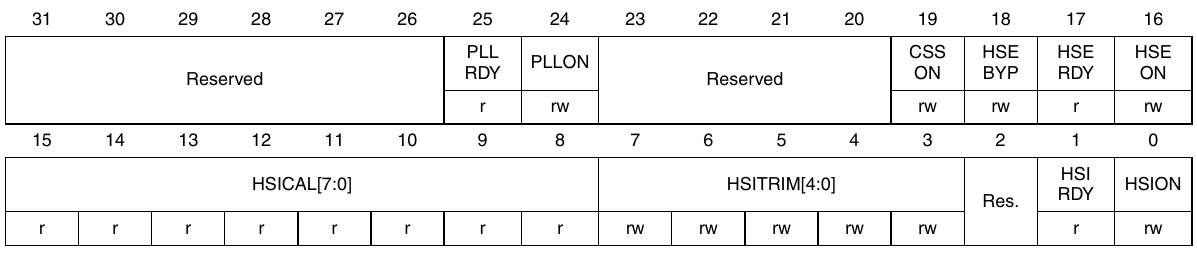
\includegraphics[width=\columnwidth]{./stm32/clocks/figs/rcc_cr}
\end{center}
\caption{RCC Clock Control Register (RCC$->$CR)}
\label{fig:rcc_cr}
\end{figure}
\item Explain the following instruction
\begin{lstlisting}
RCC->CFGR =0x00000001;	
\end{lstlisting}
\solution Fig. \ref{fig:rcc_cfgr} shows the RCC$->$CFGR register.  The above instruction makes the HSE as the system clock 
through SW = 01.
\begin{figure}[!h]
\begin{center}
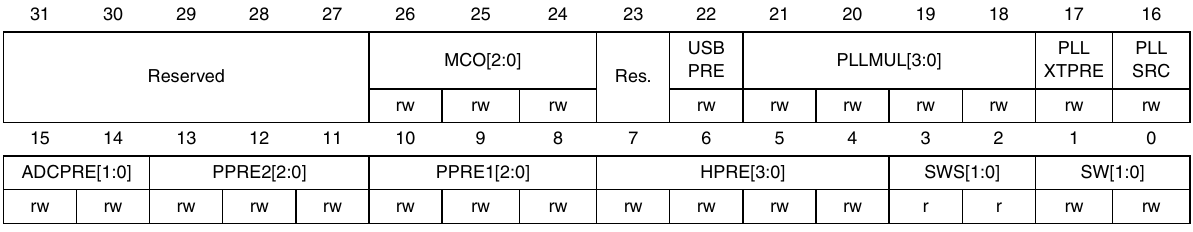
\includegraphics[width=\columnwidth]{./stm32/clocks/figs/rcc_cfgr}
\end{center}
\caption{RCC clock Configuration Register (RCC$->$CFGR)}
\label{fig:rcc_cfgr}
\end{figure}
\item Verify that HSE is the system clock by checking that SWS = 01.
\subsection{PLL}
\item Make the PLL as the system clock.
\\
\solution
\begin{lstlisting}
RCC->CFGR =0x00000010;	
\end{lstlisting}
\item Choose the PLL input as HSE.
\begin{lstlisting}
RCC->CFGR =0x00010010;	
\end{lstlisting}
\item Enable PLL
\\
\solution
\begin{lstlisting}
RCC->CR =0x01010000;
\end{lstlisting}
%
\item Execute the following code.
\begin{lstlisting}
cd /clocks/pll_systick_blink.c
\end{lstlisting}
\item Make the PLL output = 24 MHz.
\end{enumerate}

\subsection{Timers}
\begin{enumerate}[label=\arabic*.,ref=\theenumi]
%\begin{enumerate}[label=\thesubsection.\arabic*.,ref=\thesubsection.\theenumi]
\item List all the available timers in the STM32F103C8T6 blue pill.
\\
\solution  See Table \ref{table:stm32_timers}
\begin{table}[!ht]
\centering
\footnotesize
%%%%%%%%%%%%%%%%%%%%%%%%%%%%%%%%%%%%%%%%%%%%%%%%%%%%%%%%%%%%%%%%%%%%%%
%%                                                                  %%
%%  This is the header of a LaTeX2e file exported from Gnumeric.    %%
%%                                                                  %%
%%  This file can be compiled as it stands or included in another   %%
%%  LaTeX document. The table is based on the longtable package so  %%
%%  the longtable options (headers, footers...) can be set in the   %%
%%  preamble section below (see PRAMBLE).                           %%
%%                                                                  %%
%%  To include the file in another, the following two lines must be %%
%%  in the including file:                                          %%
%%        \def\inputGnumericTable{}                                 %%
%%  at the beginning of the file and:                               %%
%%        \input{name-of-this-file.tex}                             %%
%%  where the table is to be placed. Note also that the including   %%
%%  file must use the following packages for the table to be        %%
%%  rendered correctly:                                             %%
%%    \usepackage[latin1]{inputenc}                                 %%
%%    \usepackage{color}                                            %%
%%    \usepackage{array}                                            %%
%%    \usepackage{longtable}                                        %%
%%    \usepackage{calc}                                             %%
%%    \usepackage{multirow}                                         %%
%%    \usepackage{hhline}                                           %%
%%    \usepackage{ifthen}                                           %%
%%  optionally (for landscape tables embedded in another document): %%
%%    \usepackage{lscape}                                           %%
%%                                                                  %%
%%%%%%%%%%%%%%%%%%%%%%%%%%%%%%%%%%%%%%%%%%%%%%%%%%%%%%%%%%%%%%%%%%%%%%



%%  This section checks if we are begin input into another file or  %%
%%  the file will be compiled alone. First use a macro taken from   %%
%%  the TeXbook ex 7.7 (suggestion of Han-Wen Nienhuys).            %%
\def\ifundefined#1{\expandafter\ifx\csname#1\endcsname\relax}


%%  Check for the \def token for inputed files. If it is not        %%
%%  defined, the file will be processed as a standalone and the     %%
%%  preamble will be used.                                          %%
\ifundefined{inputGnumericTable}

%%  We must be able to close or not the document at the end.        %%
	\def\gnumericTableEnd{\end{document}}


%%%%%%%%%%%%%%%%%%%%%%%%%%%%%%%%%%%%%%%%%%%%%%%%%%%%%%%%%%%%%%%%%%%%%%
%%                                                                  %%
%%  This is the PREAMBLE. Change these values to get the right      %%
%%  paper size and other niceties.                                  %%
%%                                                                  %%
%%%%%%%%%%%%%%%%%%%%%%%%%%%%%%%%%%%%%%%%%%%%%%%%%%%%%%%%%%%%%%%%%%%%%%

	\documentclass[12pt%
			  %,landscape%
                    ]{report}
       \usepackage[latin1]{inputenc}
       \usepackage{fullpage}
       \usepackage{color}
       \usepackage{array}
       \usepackage{longtable}
       \usepackage{calc}
       \usepackage{multirow}
       \usepackage{hhline}
       \usepackage{ifthen}

	\begin{document}


%%  End of the preamble for the standalone. The next section is for %%
%%  documents which are included into other LaTeX2e files.          %%
\else

%%  We are not a stand alone document. For a regular table, we will %%
%%  have no preamble and only define the closing to mean nothing.   %%
    \def\gnumericTableEnd{}

%%  If we want landscape mode in an embedded document, comment out  %%
%%  the line above and uncomment the two below. The table will      %%
%%  begin on a new page and run in landscape mode.                  %%
%       \def\gnumericTableEnd{\end{landscape}}
%       \begin{landscape}


%%  End f the else clause for this file being \input.              %%
\fi

%%%%%%%%%%%%%%%%%%%%%%%%%%%%%%%%%%%%%%%%%%%%%%%%%%%%%%%%%%%%%%%%%%%%%%
%%                                                                  %%
%%  The rest is the gnumeric table, except for the closing          %%
%%  statement. Changes below will alter the table's appearance.     %%
%%                                                                  %%
%%%%%%%%%%%%%%%%%%%%%%%%%%%%%%%%%%%%%%%%%%%%%%%%%%%%%%%%%%%%%%%%%%%%%%

\providecommand{\gnumericmathit}[1]{#1} 
%%  Uncomment the next line if you would like your numbers to be in %%
%%  italics if they are italizised in the gnumeric table.           %%
%\renewcommand{\gnumericmathit}[1]{\mathit{#1}}
\providecommand{\gnumericPB}[1]%
{\let\gnumericTemp=\\#1\let\\=\gnumericTemp\hspace{0pt}}
 \ifundefined{gnumericTableWidthDefined}
        \newlength{\gnumericTableWidth}
        \newlength{\gnumericTableWidthComplete}
        \newlength{\gnumericMultiRowLength}
        \global\def\gnumericTableWidthDefined{}
 \fi
%% The following setting protects this code from babel shorthands.  %%
 \ifthenelse{\isundefined{\languageshorthands}}{}{\languageshorthands{english}}
%%  The default table format retains the relative column widths of  %%
%%  gnumeric. They can easily be changed to c, r or l. In that case %%
%%  you may want to comment out the next line and uncomment the one %%
%%  thereafter                                                      %%
\providecommand\gnumbox{\makebox[0pt]}
%%\providecommand\gnumbox[1][]{\makebox}

%% to adjust positions in multirow situations                       %%
\setlength{\bigstrutjot}{\jot}
\setlength{\extrarowheight}{\doublerulesep}

%%  The \setlongtables command keeps column widths the same across  %%
%%  pages. Simply comment out next line for varying column widths.  %%
\setlongtables

\setlength\gnumericTableWidth{%
	69pt+%
	55pt+%
	98pt+%
0pt}
\def\gumericNumCols{3}
\setlength\gnumericTableWidthComplete{\gnumericTableWidth+%
         \tabcolsep*\gumericNumCols*2+\arrayrulewidth*\gumericNumCols}
\ifthenelse{\lengthtest{\gnumericTableWidthComplete > \linewidth}}%
         {\def\gnumericScale{\ratio{\linewidth-%
                        \tabcolsep*\gumericNumCols*2-%
                        \arrayrulewidth*\gumericNumCols}%
{\gnumericTableWidth}}}%
{\def\gnumericScale{1}}

%%%%%%%%%%%%%%%%%%%%%%%%%%%%%%%%%%%%%%%%%%%%%%%%%%%%%%%%%%%%%%%%%%%%%%
%%                                                                  %%
%% The following are the widths of the various columns. We are      %%
%% defining them here because then they are easier to change.       %%
%% Depending on the cell formats we may use them more than once.    %%
%%                                                                  %%
%%%%%%%%%%%%%%%%%%%%%%%%%%%%%%%%%%%%%%%%%%%%%%%%%%%%%%%%%%%%%%%%%%%%%%

\ifthenelse{\isundefined{\gnumericColA}}{\newlength{\gnumericColA}}{}\settowidth{\gnumericColA}{\begin{tabular}{@{}p{69pt*\gnumericScale}@{}}x\end{tabular}}
\ifthenelse{\isundefined{\gnumericColB}}{\newlength{\gnumericColB}}{}\settowidth{\gnumericColB}{\begin{tabular}{@{}p{55pt*\gnumericScale}@{}}x\end{tabular}}
\ifthenelse{\isundefined{\gnumericColC}}{\newlength{\gnumericColC}}{}\settowidth{\gnumericColC}{\begin{tabular}{@{}p{98pt*\gnumericScale}@{}}x\end{tabular}}

\begin{tabular}[c]{%
	b{\gnumericColA}%
	b{\gnumericColB}%
	b{\gnumericColC}%
	}

%%%%%%%%%%%%%%%%%%%%%%%%%%%%%%%%%%%%%%%%%%%%%%%%%%%%%%%%%%%%%%%%%%%%%%
%%  The longtable options. (Caption, headers... see Goosens, p.124) %%
%	\caption{The Table Caption.}             \\	%
% \hline	% Across the top of the table.
%%  The rest of these options are table rows which are placed on    %%
%%  the first, last or every page. Use \multicolumn if you want.    %%

%%  Header for the first page.                                      %%
%	\multicolumn{3}{c}{The First Header} \\ \hline 
%	\multicolumn{1}{c}{colTag}	%Column 1
%	&\multicolumn{1}{c}{colTag}	%Column 2
%	&\multicolumn{1}{c}{colTag}	\\ \hline %Last column
%	\endfirsthead

%%  The running header definition.                                  %%
%	\hline
%	\multicolumn{3}{l}{\ldots\small\slshape continued} \\ \hline
%	\multicolumn{1}{c}{colTag}	%Column 1
%	&\multicolumn{1}{c}{colTag}	%Column 2
%	&\multicolumn{1}{c}{colTag}	\\ \hline %Last column
%	\endhead

%%  The running footer definition.                                  %%
%	\hline
%	\multicolumn{3}{r}{\small\slshape continued\ldots} \\
%	\endfoot

%%  The ending footer definition.                                   %%
%	\multicolumn{3}{c}{That's all folks} \\ \hline 
%	\endlastfoot
%%%%%%%%%%%%%%%%%%%%%%%%%%%%%%%%%%%%%%%%%%%%%%%%%%%%%%%%%%%%%%%%%%%%%%

\hhline{|-|-|-}
	 \multicolumn{1}{|p{\gnumericColA}|}%
	{\gnumericPB{\centering}\textbf{Timer}}
	&\multicolumn{1}{p{\gnumericColB}|}%
	{\gnumericPB{\centering}\textbf{Type}}
	&\multicolumn{1}{p{\gnumericColC}|}%
	{\gnumericPB{\centering}Counter Resolution}
\\
\hhline{|---|}
	 \multicolumn{1}{|p{\gnumericColA}|}%
	{\gnumericPB{\centering}Systick}
	&\multicolumn{1}{p{\gnumericColB}|}%
	{\gnumericPB{\centering}Default}
	&\multicolumn{1}{p{\gnumericColC}|}%
	{\gnumericPB{\centering}24 bit}
\\
\hhline{|---|}
	 \multicolumn{1}{|p{\gnumericColA}|}%
	{\gnumericPB{\centering}Independent}
	&\multicolumn{1}{p{\gnumericColB}|}%
	{\gnumericPB{\centering}Watchdog}
	&\multicolumn{1}{p{\gnumericColC}|}%
	{\gnumericPB{\centering}12 bit}
\\
\hhline{|---|}
	 \multicolumn{1}{|p{\gnumericColA}|}%
	{\gnumericPB{\centering}Window}
	&\multicolumn{1}{p{\gnumericColB}|}%
	{\gnumericPB{\centering}Watchdog}
	&\multicolumn{1}{p{\gnumericColC}|}%
	{\gnumericPB{\centering}7 bit}
\\
\hhline{|---|}
	 \multicolumn{1}{|p{\gnumericColA}|}%
	{\gnumericPB{\centering}TIM1}
	&\multicolumn{1}{p{\gnumericColB}|}%
	{\gnumericPB{\centering}Advanced}
	&\multicolumn{1}{p{\gnumericColC}|}%
	{\setlength{\gnumericMultiRowLength}{0pt}%
	 \addtolength{\gnumericMultiRowLength}{\gnumericColC}%
	 \multirow{4}[2]{\gnumericMultiRowLength}{\parbox{\gnumericMultiRowLength}{%
	 \gnumericPB{\centering}16 bit}}}
\\
\hhline{|--|~}
	 \multicolumn{1}{|p{\gnumericColA}|}%
	{\gnumericPB{\centering}TIM2}
	&\multicolumn{1}{p{\gnumericColB}|}%
	{\setlength{\gnumericMultiRowLength}{0pt}%
	 \addtolength{\gnumericMultiRowLength}{\gnumericColB}%
	 \multirow{3}[1]{\gnumericMultiRowLength}{\parbox{\gnumericMultiRowLength}{%
	 \gnumericPB{\centering}General Purpose}}}
	&\multicolumn{1}{p{\gnumericColC}|}%
	{}
\\
\hhline{|-|~~}
	 \multicolumn{1}{|p{\gnumericColA}|}%
	{\gnumericPB{\centering}TIM3}
	&\multicolumn{1}{p{\gnumericColB}|}%
	{}
	&\multicolumn{1}{p{\gnumericColC}|}%
	{}
\\
\hhline{|-|~~}
	 \multicolumn{1}{|p{\gnumericColA}|}%
	{\gnumericPB{\centering}TIM4}
	&\multicolumn{1}{p{\gnumericColB}|}%
	{}
	&\multicolumn{1}{p{\gnumericColC}|}%
	{}
\\
\hhline{|-|-|-|}
\end{tabular}

\ifthenelse{\isundefined{\languageshorthands}}{}{\languageshorthands{\languagename}}
\gnumericTableEnd

\caption{STM32F103C8T6 Timer Types.}
\label{table:stm32_timers}
\end{table}

\subsection{Systick timer}
\item The Systick timer is the default timer available on all ARM chips. 
\item Make connections as shown in Table \ref{table:systick_pins}.
\begin{table}[!ht]
\centering
\footnotesize
%%%%%%%%%%%%%%%%%%%%%%%%%%%%%%%%%%%%%%%%%%%%%%%%%%%%%%%%%%%%%%%%%%%%%%
%%                                                                  %%
%%  This is the header of a LaTeX2e file exported from Gnumeric.    %%
%%                                                                  %%
%%  This file can be compiled as it stands or included in another   %%
%%  LaTeX document. The table is based on the longtable package so  %%
%%  the longtable options (headers, footers...) can be set in the   %%
%%  preamble section below (see PRAMBLE).                           %%
%%                                                                  %%
%%  To include the file in another, the following two lines must be %%
%%  in the including file:                                          %%
%%        \def\inputGnumericTable{}                                 %%
%%  at the beginning of the file and:                               %%
%%        \input{name-of-this-file.tex}                             %%
%%  where the table is to be placed. Note also that the including   %%
%%  file must use the following packages for the table to be        %%
%%  rendered correctly:                                             %%
%%    \usepackage[latin1]{inputenc}                                 %%
%%    \usepackage{color}                                            %%
%%    \usepackage{array}                                            %%
%%    \usepackage{longtable}                                        %%
%%    \usepackage{calc}                                             %%
%%    \usepackage{multirow}                                         %%
%%    \usepackage{hhline}                                           %%
%%    \usepackage{ifthen}                                           %%
%%  optionally (for landscape tables embedded in another document): %%
%%    \usepackage{lscape}                                           %%
%%                                                                  %%
%%%%%%%%%%%%%%%%%%%%%%%%%%%%%%%%%%%%%%%%%%%%%%%%%%%%%%%%%%%%%%%%%%%%%%



%%  This section checks if we are begin input into another file or  %%
%%  the file will be compiled alone. First use a macro taken from   %%
%%  the TeXbook ex 7.7 (suggestion of Han-Wen Nienhuys).            %%
\def\ifundefined#1{\expandafter\ifx\csname#1\endcsname\relax}


%%  Check for the \def token for inputed files. If it is not        %%
%%  defined, the file will be processed as a standalone and the     %%
%%  preamble will be used.                                          %%
\ifundefined{inputGnumericTable}

%%  We must be able to close or not the document at the end.        %%
	\def\gnumericTableEnd{\end{document}}


%%%%%%%%%%%%%%%%%%%%%%%%%%%%%%%%%%%%%%%%%%%%%%%%%%%%%%%%%%%%%%%%%%%%%%
%%                                                                  %%
%%  This is the PREAMBLE. Change these values to get the right      %%
%%  paper size and other niceties.                                  %%
%%                                                                  %%
%%%%%%%%%%%%%%%%%%%%%%%%%%%%%%%%%%%%%%%%%%%%%%%%%%%%%%%%%%%%%%%%%%%%%%

	\documentclass[12pt%
			  %,landscape%
                    ]{report}
       \usepackage[latin1]{inputenc}
       \usepackage{fullpage}
       \usepackage{color}
       \usepackage{array}
       \usepackage{longtable}
       \usepackage{calc}
       \usepackage{multirow}
       \usepackage{hhline}
       \usepackage{ifthen}

	\begin{document}


%%  End of the preamble for the standalone. The next section is for %%
%%  documents which are included into other LaTeX2e files.          %%
\else

%%  We are not a stand alone document. For a regular table, we will %%
%%  have no preamble and only define the closing to mean nothing.   %%
    \def\gnumericTableEnd{}

%%  If we want landscape mode in an embedded document, comment out  %%
%%  the line above and uncomment the two below. The table will      %%
%%  begin on a new page and run in landscape mode.                  %%
%       \def\gnumericTableEnd{\end{landscape}}
%       \begin{landscape}


%%  End f the else clause for this file being \input.              %%
\fi

%%%%%%%%%%%%%%%%%%%%%%%%%%%%%%%%%%%%%%%%%%%%%%%%%%%%%%%%%%%%%%%%%%%%%%
%%                                                                  %%
%%  The rest is the gnumeric table, except for the closing          %%
%%  statement. Changes below will alter the table's appearance.     %%
%%                                                                  %%
%%%%%%%%%%%%%%%%%%%%%%%%%%%%%%%%%%%%%%%%%%%%%%%%%%%%%%%%%%%%%%%%%%%%%%

\providecommand{\gnumericmathit}[1]{#1} 
%%  Uncomment the next line if you would like your numbers to be in %%
%%  italics if they are italizised in the gnumeric table.           %%
%\renewcommand{\gnumericmathit}[1]{\mathit{#1}}
\providecommand{\gnumericPB}[1]%
{\let\gnumericTemp=\\#1\let\\=\gnumericTemp\hspace{0pt}}
 \ifundefined{gnumericTableWidthDefined}
        \newlength{\gnumericTableWidth}
        \newlength{\gnumericTableWidthComplete}
        \newlength{\gnumericMultiRowLength}
        \global\def\gnumericTableWidthDefined{}
 \fi
%% The following setting protects this code from babel shorthands.  %%
 \ifthenelse{\isundefined{\languageshorthands}}{}{\languageshorthands{english}}
%%  The default table format retains the relative column widths of  %%
%%  gnumeric. They can easily be changed to c, r or l. In that case %%
%%  you may want to comment out the next line and uncomment the one %%
%%  thereafter                                                      %%
\providecommand\gnumbox{\makebox[0pt]}
%%\providecommand\gnumbox[1][]{\makebox}

%% to adjust positions in multirow situations                       %%
\setlength{\bigstrutjot}{\jot}
\setlength{\extrarowheight}{\doublerulesep}

%%  The \setlongtables command keeps column widths the same across  %%
%%  pages. Simply comment out next line for varying column widths.  %%
\setlongtables

\setlength\gnumericTableWidth{%
	40pt+%
	117pt+%
0pt}
\def\gumericNumCols{2}
\setlength\gnumericTableWidthComplete{\gnumericTableWidth+%
         \tabcolsep*\gumericNumCols*2+\arrayrulewidth*\gumericNumCols}
\ifthenelse{\lengthtest{\gnumericTableWidthComplete > \linewidth}}%
         {\def\gnumericScale{\ratio{\linewidth-%
                        \tabcolsep*\gumericNumCols*2-%
                        \arrayrulewidth*\gumericNumCols}%
{\gnumericTableWidth}}}%
{\def\gnumericScale{1}}

%%%%%%%%%%%%%%%%%%%%%%%%%%%%%%%%%%%%%%%%%%%%%%%%%%%%%%%%%%%%%%%%%%%%%%
%%                                                                  %%
%% The following are the widths of the various columns. We are      %%
%% defining them here because then they are easier to change.       %%
%% Depending on the cell formats we may use them more than once.    %%
%%                                                                  %%
%%%%%%%%%%%%%%%%%%%%%%%%%%%%%%%%%%%%%%%%%%%%%%%%%%%%%%%%%%%%%%%%%%%%%%

\ifthenelse{\isundefined{\gnumericColA}}{\newlength{\gnumericColA}}{}\settowidth{\gnumericColA}{\begin{tabular}{@{}p{40pt*\gnumericScale}@{}}x\end{tabular}}
\ifthenelse{\isundefined{\gnumericColB}}{\newlength{\gnumericColB}}{}\settowidth{\gnumericColB}{\begin{tabular}{@{}p{117pt*\gnumericScale}@{}}x\end{tabular}}

\begin{tabular}[c]{%
	b{\gnumericColA}%
	b{\gnumericColB}%
	}

%%%%%%%%%%%%%%%%%%%%%%%%%%%%%%%%%%%%%%%%%%%%%%%%%%%%%%%%%%%%%%%%%%%%%%
%%  The longtable options. (Caption, headers... see Goosens, p.124) %%
%	\caption{The Table Caption.}             \\	%
% \hline	% Across the top of the table.
%%  The rest of these options are table rows which are placed on    %%
%%  the first, last or every page. Use \multicolumn if you want.    %%

%%  Header for the first page.                                      %%
%	\multicolumn{2}{c}{The First Header} \\ \hline 
%	\multicolumn{1}{c}{colTag}	%Column 1
%	&\multicolumn{1}{c}{colTag}	\\ \hline %Last column
%	\endfirsthead

%%  The running header definition.                                  %%
%	\hline
%	\multicolumn{2}{l}{\ldots\small\slshape continued} \\ \hline
%	\multicolumn{1}{c}{colTag}	%Column 1
%	&\multicolumn{1}{c}{colTag}	\\ \hline %Last column
%	\endhead

%%  The running footer definition.                                  %%
%	\hline
%	\multicolumn{2}{r}{\small\slshape continued\ldots} \\
%	\endfoot

%%  The ending footer definition.                                   %%
%	\multicolumn{2}{c}{That's all folks} \\ \hline 
%	\endlastfoot
%%%%%%%%%%%%%%%%%%%%%%%%%%%%%%%%%%%%%%%%%%%%%%%%%%%%%%%%%%%%%%%%%%%%%%

\hhline{|-|-}
	 \multicolumn{1}{|p{\gnumericColA}|}%
	{\gnumericPB{\centering}\gnumbox{\textbf{STM32}}}
	&\multicolumn{1}{p{\gnumericColB}|}%
	{\gnumericPB{\centering}\gnumbox{\textbf{Seven Segment Display}}}
\\
\hhline{|--|}
	 \multicolumn{1}{|p{\gnumericColA}|}%
	{\gnumericPB{\centering}\gnumbox{3.3V}}
	&\multicolumn{1}{p{\gnumericColB}|}%
	{\gnumericPB{\centering}\gnumbox{COM (through resistor)}}
\\
\hhline{|--|}
	 \multicolumn{1}{|p{\gnumericColA}|}%
	{\gnumericPB{\centering}\gnumbox{PA1}}
	&\multicolumn{1}{p{\gnumericColB}|}%
	{\gnumericPB{\centering}\gnumbox{DOT}}
\\
\hhline{|-|-|}
\end{tabular}

\ifthenelse{\isundefined{\languageshorthands}}{}{\languageshorthands{\languagename}}
\gnumericTableEnd

\caption{Pin Connections}
\label{table:systick_pins}
\end{table}
\item Execute the program in 
\begin{lstlisting}
timers/codes/blink_systick.c
\end{lstlisting}
\item The default clock is the HSI 8MHz RC.  Find the number of clock cycles required for a 1 s delay.
\\
\solution The time period is
\begin{equation}
T = \frac{1}{8}\mu s = 1 \text{ cycle}
\end{equation}
Thus, the number of cycles required for 1 s delay is
\begin{equation}
1 \text{ second} = 8000000 \text{ cycles}
\end{equation}
\item List the SysTick registers.
\\
\solution See Table \ref{table:systick_reg}.
\begin{table}[!ht]
\footnotesize
\centering
%%%%%%%%%%%%%%%%%%%%%%%%%%%%%%%%%%%%%%%%%%%%%%%%%%%%%%%%%%%%%%%%%%%%%%
%%                                                                  %%
%%  This is the header of a LaTeX2e file exported from Gnumeric.    %%
%%                                                                  %%
%%  This file can be compiled as it stands or included in another   %%
%%  LaTeX document. The table is based on the longtable package so  %%
%%  the longtable options (headers, footers...) can be set in the   %%
%%  preamble section below (see PRAMBLE).                           %%
%%                                                                  %%
%%  To include the file in another, the following two lines must be %%
%%  in the including file:                                          %%
%%        \def\inputGnumericTable{}                                 %%
%%  at the beginning of the file and:                               %%
%%        \input{name-of-this-file.tex}                             %%
%%  where the table is to be placed. Note also that the including   %%
%%  file must use the following packages for the table to be        %%
%%  rendered correctly:                                             %%
%%    \usepackage[latin1]{inputenc}                                 %%
%%    \usepackage{color}                                            %%
%%    \usepackage{array}                                            %%
%%    \usepackage{longtable}                                        %%
%%    \usepackage{calc}                                             %%
%%    \usepackage{multirow}                                         %%
%%    \usepackage{hhline}                                           %%
%%    \usepackage{ifthen}                                           %%
%%  optionally (for landscape tables embedded in another document): %%
%%    \usepackage{lscape}                                           %%
%%                                                                  %%
%%%%%%%%%%%%%%%%%%%%%%%%%%%%%%%%%%%%%%%%%%%%%%%%%%%%%%%%%%%%%%%%%%%%%%



%%  This section checks if we are begin input into another file or  %%
%%  the file will be compiled alone. First use a macro taken from   %%
%%  the TeXbook ex 7.7 (suggestion of Han-Wen Nienhuys).            %%
\def\ifundefined#1{\expandafter\ifx\csname#1\endcsname\relax}


%%  Check for the \def token for inputed files. If it is not        %%
%%  defined, the file will be processed as a standalone and the     %%
%%  preamble will be used.                                          %%
\ifundefined{inputGnumericTable}

%%  We must be able to close or not the document at the end.        %%
	\def\gnumericTableEnd{\end{document}}


%%%%%%%%%%%%%%%%%%%%%%%%%%%%%%%%%%%%%%%%%%%%%%%%%%%%%%%%%%%%%%%%%%%%%%
%%                                                                  %%
%%  This is the PREAMBLE. Change these values to get the right      %%
%%  paper size and other niceties.                                  %%
%%                                                                  %%
%%%%%%%%%%%%%%%%%%%%%%%%%%%%%%%%%%%%%%%%%%%%%%%%%%%%%%%%%%%%%%%%%%%%%%

	\documentclass[12pt%
			  %,landscape%
                    ]{report}
       \usepackage[latin1]{inputenc}
       \usepackage{fullpage}
       \usepackage{color}
       \usepackage{array}
       \usepackage{longtable}
       \usepackage{calc}
       \usepackage{multirow}
       \usepackage{hhline}
       \usepackage{ifthen}

	\begin{document}


%%  End of the preamble for the standalone. The next section is for %%
%%  documents which are included into other LaTeX2e files.          %%
\else

%%  We are not a stand alone document. For a regular table, we will %%
%%  have no preamble and only define the closing to mean nothing.   %%
    \def\gnumericTableEnd{}

%%  If we want landscape mode in an embedded document, comment out  %%
%%  the line above and uncomment the two below. The table will      %%
%%  begin on a new page and run in landscape mode.                  %%
%       \def\gnumericTableEnd{\end{landscape}}
%       \begin{landscape}


%%  End f the else clause for this file being \input.              %%
\fi

%%%%%%%%%%%%%%%%%%%%%%%%%%%%%%%%%%%%%%%%%%%%%%%%%%%%%%%%%%%%%%%%%%%%%%
%%                                                                  %%
%%  The rest is the gnumeric table, except for the closing          %%
%%  statement. Changes below will alter the table's appearance.     %%
%%                                                                  %%
%%%%%%%%%%%%%%%%%%%%%%%%%%%%%%%%%%%%%%%%%%%%%%%%%%%%%%%%%%%%%%%%%%%%%%

\providecommand{\gnumericmathit}[1]{#1} 
%%  Uncomment the next line if you would like your numbers to be in %%
%%  italics if they are italizised in the gnumeric table.           %%
%\renewcommand{\gnumericmathit}[1]{\mathit{#1}}
\providecommand{\gnumericPB}[1]%
{\let\gnumericTemp=\\#1\let\\=\gnumericTemp\hspace{0pt}}
 \ifundefined{gnumericTableWidthDefined}
        \newlength{\gnumericTableWidth}
        \newlength{\gnumericTableWidthComplete}
        \newlength{\gnumericMultiRowLength}
        \global\def\gnumericTableWidthDefined{}
 \fi
%% The following setting protects this code from babel shorthands.  %%
 \ifthenelse{\isundefined{\languageshorthands}}{}{\languageshorthands{english}}
%%  The default table format retains the relative column widths of  %%
%%  gnumeric. They can easily be changed to c, r or l. In that case %%
%%  you may want to comment out the next line and uncomment the one %%
%%  thereafter                                                      %%
\providecommand\gnumbox{\makebox[0pt]}
%%\providecommand\gnumbox[1][]{\makebox}

%% to adjust positions in multirow situations                       %%
\setlength{\bigstrutjot}{\jot}
\setlength{\extrarowheight}{\doublerulesep}

%%  The \setlongtables command keeps column widths the same across  %%
%%  pages. Simply comment out next line for varying column widths.  %%
\setlongtables

\setlength\gnumericTableWidth{%
	149pt+%
	89pt+%
	85pt+%
0pt}
\def\gumericNumCols{3}
\setlength\gnumericTableWidthComplete{\gnumericTableWidth+%
         \tabcolsep*\gumericNumCols*2+\arrayrulewidth*\gumericNumCols}
\ifthenelse{\lengthtest{\gnumericTableWidthComplete > \linewidth}}%
         {\def\gnumericScale{\ratio{\linewidth-%
                        \tabcolsep*\gumericNumCols*2-%
                        \arrayrulewidth*\gumericNumCols}%
{\gnumericTableWidth}}}%
{\def\gnumericScale{1}}

%%%%%%%%%%%%%%%%%%%%%%%%%%%%%%%%%%%%%%%%%%%%%%%%%%%%%%%%%%%%%%%%%%%%%%
%%                                                                  %%
%% The following are the widths of the various columns. We are      %%
%% defining them here because then they are easier to change.       %%
%% Depending on the cell formats we may use them more than once.    %%
%%                                                                  %%
%%%%%%%%%%%%%%%%%%%%%%%%%%%%%%%%%%%%%%%%%%%%%%%%%%%%%%%%%%%%%%%%%%%%%%

\ifthenelse{\isundefined{\gnumericColA}}{\newlength{\gnumericColA}}{}\settowidth{\gnumericColA}{\begin{tabular}{@{}p{149pt*\gnumericScale}@{}}x\end{tabular}}
\ifthenelse{\isundefined{\gnumericColB}}{\newlength{\gnumericColB}}{}\settowidth{\gnumericColB}{\begin{tabular}{@{}p{89pt*\gnumericScale}@{}}x\end{tabular}}
\ifthenelse{\isundefined{\gnumericColC}}{\newlength{\gnumericColC}}{}\settowidth{\gnumericColC}{\begin{tabular}{@{}p{85pt*\gnumericScale}@{}}x\end{tabular}}

\begin{tabular}[c]{%
	b{\gnumericColA}%
	b{\gnumericColB}%
	b{\gnumericColC}%
	}

%%%%%%%%%%%%%%%%%%%%%%%%%%%%%%%%%%%%%%%%%%%%%%%%%%%%%%%%%%%%%%%%%%%%%%
%%  The longtable options. (Caption, headers... see Goosens, p.124) %%
%	\caption{The Table Caption.}             \\	%
% \hline	% Across the top of the table.
%%  The rest of these options are table rows which are placed on    %%
%%  the first, last or every page. Use \multicolumn if you want.    %%

%%  Header for the first page.                                      %%
%	\multicolumn{3}{c}{The First Header} \\ \hline 
%	\multicolumn{1}{c}{colTag}	%Column 1
%	&\multicolumn{1}{c}{colTag}	%Column 2
%	&\multicolumn{1}{c}{colTag}	\\ \hline %Last column
%	\endfirsthead

%%  The running header definition.                                  %%
%	\hline
%	\multicolumn{3}{l}{\ldots\small\slshape continued} \\ \hline
%	\multicolumn{1}{c}{colTag}	%Column 1
%	&\multicolumn{1}{c}{colTag}	%Column 2
%	&\multicolumn{1}{c}{colTag}	\\ \hline %Last column
%	\endhead

%%  The running footer definition.                                  %%
%	\hline
%	\multicolumn{3}{r}{\small\slshape continued\ldots} \\
%	\endfoot

%%  The ending footer definition.                                   %%
%	\multicolumn{3}{c}{That's all folks} \\ \hline 
%	\endlastfoot
%%%%%%%%%%%%%%%%%%%%%%%%%%%%%%%%%%%%%%%%%%%%%%%%%%%%%%%%%%%%%%%%%%%%%%

\hhline{|-|-|-}
	 \multicolumn{1}{|p{\gnumericColA}|}%
	{\gnumericPB{\raggedright}\gnumbox[l]{\textbf{Register}}}
	&\multicolumn{1}{p{\gnumericColB}|}%
	{\gnumericPB{\raggedright}\gnumbox[l]{\textbf{Command}}}
	&\multicolumn{1}{p{\gnumericColC}|}%
	{\gnumericPB{\raggedright}\gnumbox[l]{\textbf{Purpose}}}
\\
\hhline{|---|}
	 \multicolumn{1}{|p{\gnumericColA}|}%
	{\gnumericPB{\raggedright}\gnumbox[l]{SysTick Control and Status}}
	&\multicolumn{1}{p{\gnumericColB}|}%
	{\gnumericPB{\raggedright}\gnumbox[l]{SysTick-$>$CTRL}}
	&\multicolumn{1}{p{\gnumericColC}|}%
	{\gnumericPB{\raggedright}\gnumbox[l]{Timer control}}
\\
\hhline{|---|}
	 \multicolumn{1}{|p{\gnumericColA}|}%
	{\gnumericPB{\raggedright}\gnumbox[l]{SysTick Reload Value}}
	&\multicolumn{1}{p{\gnumericColB}|}%
	{\gnumericPB{\raggedright}\gnumbox[l]{SysTick-$>$LOAD}}
	&\multicolumn{1}{p{\gnumericColC}|}%
	{\gnumericPB{\raggedright}\gnumbox[l]{Timer Count}}
\\
\hhline{|---|}
	 \multicolumn{1}{|p{\gnumericColA}|}%
	{\gnumericPB{\raggedright}\gnumbox[l]{SysTick Current Value}}
	&\multicolumn{1}{p{\gnumericColB}|}%
	{\gnumericPB{\raggedright}\gnumbox[l]{SysTick-$>$VAL}}
	&\multicolumn{1}{p{\gnumericColC}|}%
	{\gnumericPB{\raggedright}\gnumbox[l]{Timer Initialize}}
\\
\hhline{|---|}
	 \multicolumn{1}{|p{\gnumericColA}|}%
	{\gnumericPB{\raggedright}\gnumbox[l]{SysTick Calibration Value}}
	&\multicolumn{1}{p{\gnumericColB}|}%
	{}
	&\multicolumn{1}{p{\gnumericColC}|}%
	{}
\\
\hhline{|-|-|-|}
\end{tabular}

\ifthenelse{\isundefined{\languageshorthands}}{}{\languageshorthands{\languagename}}
\gnumericTableEnd

\caption{Systick Registers}
\label{table:systick_reg}
\end{table}
\item What do the following instructions do?
\begin{lstlisting}
SysTick->LOAD = 4000000;
SysTick->VAL = 0;
\end{lstlisting}
\solution See Table \ref{table:systick_reg} for details.  These two instructions ask the SysTick timer to count down from 4000000 to 0.  
\item Explain the following instruction.
\begin{lstlisting}
while(!(SysTick->CTRL & 0x00010000));
\end{lstlisting}
\solution Fig. \ref{fig:systick_ctrl} shows the SysTick CTRL register.    0x00010000 is used in the above command to mask all the bits except for bit 16, which
is the COUNTFLAG.  The \textbf{while} loop will stop once COUNTFLAG = 0. The while loop is used for the delay.
\begin{figure}[!ht]
\begin{center}
%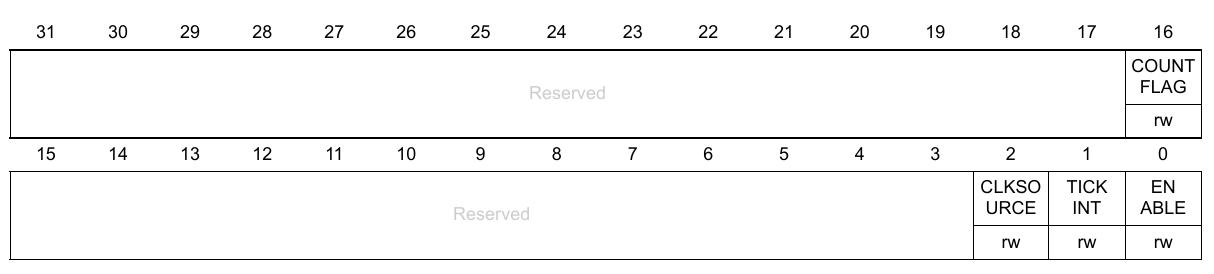
\includegraphics[width=\columnwidth]{./stm32/timers/figs/systick_ctrl.eps}
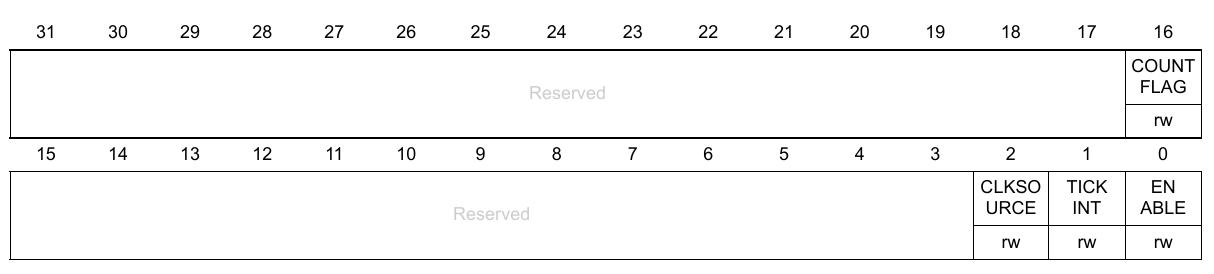
\includegraphics[width=\columnwidth]{stm32/timers/figs/systick_ctrl}
\end{center}
\caption{Control Register (CTRL)}
\label{fig:systick_ctrl}
\end{figure}
\item What does the following instruciton do?
\begin{lstlisting}
SysTick->CTRL = 0x00000005;	//8MHz clock
\end{lstlisting}
\solution From Fig. \ref{fig:systick_ctrl}, ENABLE = 1 enables the counter (for delay) and CLKSOURCE = 1 enables the 8 MHz internal RC clock.
\item Obtain a 1 MHz clock. 
\\
\solution CLKSOURCE = 1 results in the $\frac{\text{Processor Clock}}{8} = 1$ MHz clock.
\begin{lstlisting}
SysTick->CTRL = 0x00000001;	//1MHz clock
\end{lstlisting}
\item Obtain a delay of 1 second using the 1 MHz clock.
\subsection{TIMER-1}
\item Make the connections according to Table \ref{table:systick_pins}.  Execute the following program
\begin{lstlisting}
cd /timers/timer1_blink.c
\end{lstlisting}
\label{prob:APB2_TIM1}
\item Enable Timer1 through RCC.
\\
\solution 
\begin{lstlisting}
RCC->APB2ENR |= RCC_APB2ENR_TIM1EN;  
\end{lstlisting}
\item Select the HSI clock of 8 MHz as TIM1 clock.
\\
\solution See Fig.  \ref{fig:smcr} for register. SMS=000 implies that the TIM1 will be controlled by the internal clock.
\begin{lstlisting}
TIM1->SMCR  = 0;
\end{lstlisting}
\begin{figure}[!ht]
%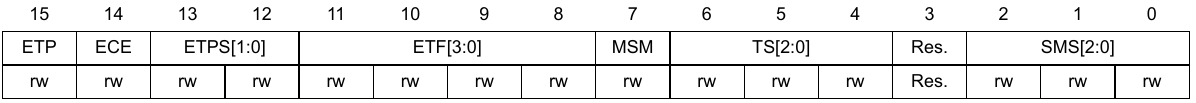
\includegraphics[width=\columnwidth]{./stm32/timers/figs/smcr.eps}
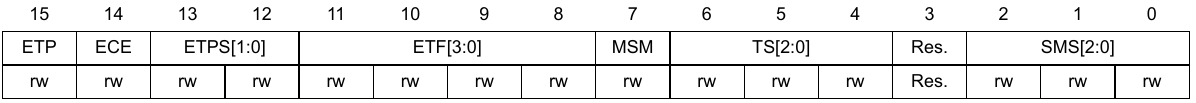
\includegraphics[width=\columnwidth]{stm32/timers/figs/smcr}
\caption{Slave Mode Control Register (SMCR)}
\label{fig:smcr}
\end{figure}
\item What does the following instruction do?
\begin{lstlisting}
TIM1->CR1 	= 0x0001;
\end{lstlisting}
\solution Fig. \ref{fig:cr1} shows the control register 1 (CR1). CEN=1 enables the counter.
\begin{figure}[!ht]
\begin{center}
%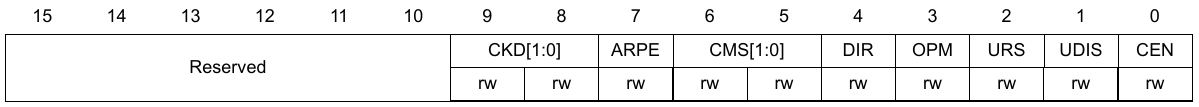
\includegraphics[width=\columnwidth]{./stm32/timers/figs/cr1.eps}
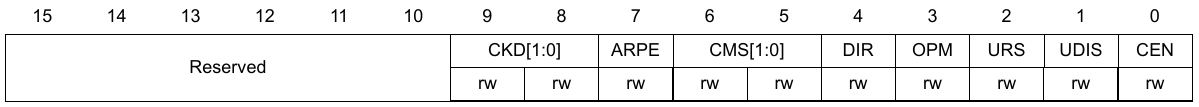
\includegraphics[width=\columnwidth]{stm32/timers/figs/cr1}
\end{center}
\caption{Control Register 1 (CR1)}
\label{fig:cr1}
\end{figure}
\item Make TIM1 clock = 2 KHz.
\\
\solution Through the following command,
\begin{lstlisting}
TIM1->PSC	= 3999;
\end{lstlisting}
\begin{equation}
TIM1\_CLK = \frac{HSI\_CLK}{TIM1->PSC + 1} = \frac{8000000}{4000}
\end{equation}
Fig. \ref{fig:psc} shows the TIM1$->$PSC (prescalar) register.
\begin{figure}[!ht]
\begin{center}
%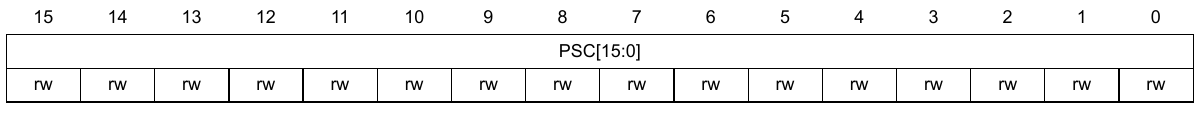
\includegraphics[width=\columnwidth]{./stm32/timers/figs/psc.eps}
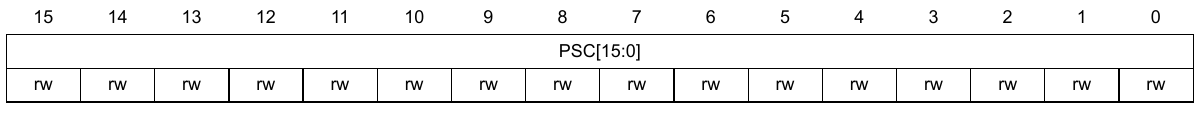
\includegraphics[width=\columnwidth]{stm32/timers/figs/psc}
\end{center}
\caption{Prescalar (PSC)}
\label{fig:psc}
\end{figure}
\item What is the maximum value that can be stored in TIM1$->$PSC?
\item Make TIM1 count 1000 cycles of the 2 KHz TIM1 clock.
\\
\solution 
\begin{lstlisting}
TIM1->ARR 	= 999;	
\end{lstlisting}
\item Like the PSC, the ARR (auto reload register) is also of length 16 bits and used for factoring the clock.
\item What do the following instructions do?
\begin{lstlisting}
if(TIM1->SR & 0x0001)//check if ARR count complete
{
	TIM1->SR &= ~0x0001;//clear status register SR
	GPIOA->ODR ^= (1 << 1);//blink LED through PA1
}
\end{lstlisting}
\solution Once the TIM1 counter counts from 0 to TIM1$->$ARR=999, it resets and starts counting again to 999.  At the time of
reset, the LSB of TIM1$->$SR = 1.  The \textbf{if} command checks this and when this condition is satisfied, TIM1$->$SR is cleared
and PA1 is toggled.  This process keeps repeating. This results in a PA1  output of 1 and 0 with frequency
\begin{align}
\frac{HSI\_CLK}{\brak{TIM1->PSC + 1}\brak{TIM1->ARR + 1}} 
= \frac{8000000}{4000\times 1000} = 2 \text{ Hz}
\end{align}
\item How would you use the repetition counter (RCR) to do the above?
\\
\solution The following instructions
\begin{lstlisting}
	TIM1->SMCR  = 0;	//Internal clock, 8MHz	
	TIM1->PSC	= 999;	//Prescalar, dividing clock by 1000
	TIM1->CR1 	= 0x0001;	//enable Timer1
	TIM1->ARR 	= 999;	//Load Count
	TIM1->RCR 	= 3;	//Load Repetition Count	
\end{lstlisting}
lead to
\begin{multline}
\frac{HSI\_CLK}{\brak{TIM1->PSC + 1}\brak{TIM1->ARR + 1}\brak{TIM1->RCR + 1}} 
\\
= \frac{8000000}{4000\times 1000} = 2 \text{ Hz}
\end{multline}
TIM1$->$RCR keeps track of the number of times the counter has overflowed. Fig. \ref{fig:rcr} shows the repetition counter register.
\begin{figure}[!h]
\begin{center}
%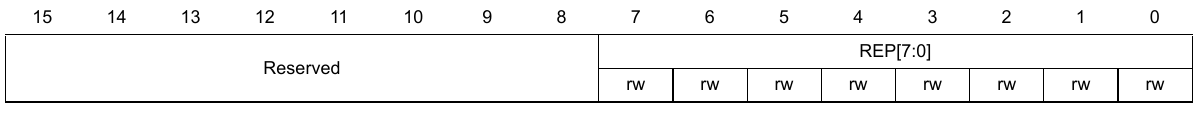
\includegraphics[width=\columnwidth]{./stm32/timers/figs/rcr.eps}
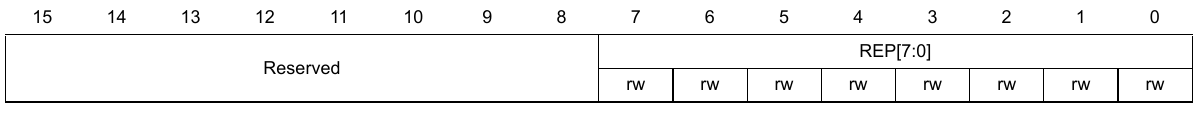
\includegraphics[width=\columnwidth]{stm32/timers/figs/rcr}
\end{center}
\caption{Repition Counter (RCR)}
\label{fig:rcr}
\end{figure}
\item What is the maximum value of TIM1$->$RCR?
\item What is the function of TIM1$->$SR?
\\
\solution The status register (SR) is shown in Fig. \ref{fig:sr}. The UIF flag is 1 if the RCR overflows.
\begin{figure}[!h]
\begin{center}
%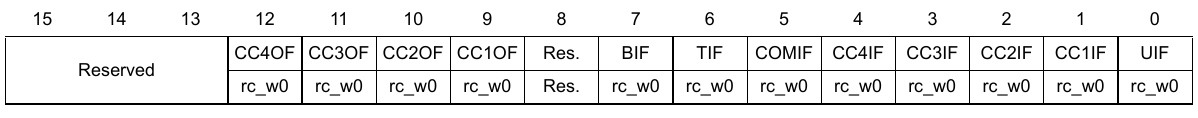
\includegraphics[width=\columnwidth]{./stm32/timers/figs/sr.eps}
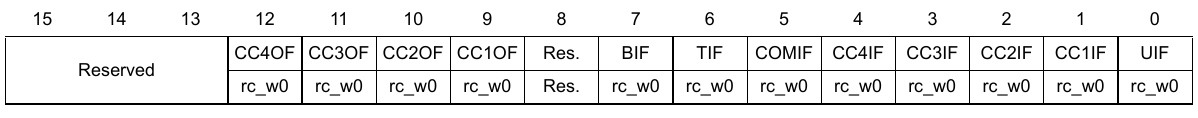
\includegraphics[width=\columnwidth]{stm32/timers/figs/sr}
\end{center}
\caption{Staus Register (SR)}
\label{fig:sr}
\end{figure}

\subsection{TIMER-2}
\item Blink an LED with TIM2.
\\
\solution 
\begin{lstlisting}
timers/codes/timer2_blink.c
\end{lstlisting}
\item In the above code, 
\begin{lstlisting}
RCC->APB1ENR |= RCC_APB1ENR_TIM2EN;
\end{lstlisting}
is used for enabling TIM2. Note that for TIM1, APB2 was used instead of APB1 in Problem \ref{prob:APB2_TIM1}.  Explain.
\\
\solution Advanced Peripheral Bus 1 (APB1) and Advanced Peripheral Bus 2 (APB2) are connected to the Direct Memory Access (DMA) module, SRAM, peripherals like GPIOs, ADC, timers, etc. and Cortex core. APB1 has a maximum operating frequency of 36MHz while the maximum operating frequency of APB2  is 72MHz. That is why GPIOs are connected to APB2 bus instead of APB1 or any other bus and STM32 GPIOs can achieve 50MHz switching speed. APB1 bus mostly serves communication and timer modules of the STM32. 
\item Mention any major difference between TIM1 and TIM2.
\\
\solution TIM1 is an advanced timer while TIM2 is a general purpose timer.  One major difference between the two is that TIM2 does not have RCR.
\subsection{Master-Slave Configuration}
\subsubsection{Blink}
\item Execute the following program.
\begin{lstlisting}
timers/codes/master1_slave2_blink.c
\end{lstlisting}
\item List the instructions for setting up TIM1 as master and TIM2 as slave. TIM1 should be a prescalar for TIM2.
\\
\solution The MMS bits can be seen in the CR2 register is shown in Fig. \ref{fig:cr2}. The TS and SMS bits are visible in the SMCR register
in Fig. \ref{fig:smcr}. 
\begin{lstlisting}
TIM1->CR2	= 0x0020;//MMS = 010
TIM2->SMCR	= 0x0007;//TS = 000, SMS = 111	
\end{lstlisting}
%
\begin{figure}[!h]
\begin{center}
%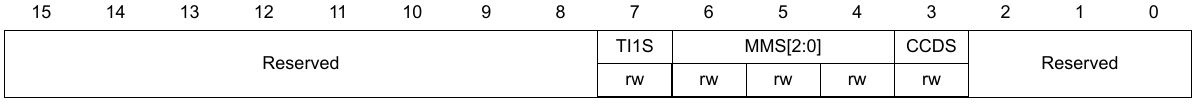
\includegraphics[width=\columnwidth]{./stm32/timers/figs/cr2.eps}
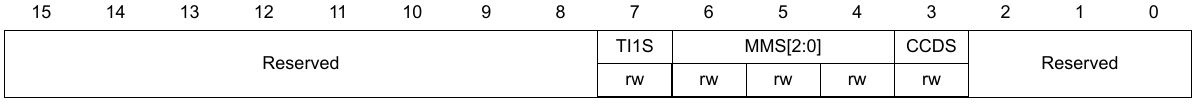
\includegraphics[width=\columnwidth]{stm32/timers/figs/cr2}
\end{center}
\caption{Control Register 2 (CR2)}
\label{fig:cr2}
\end{figure}
%
\subsubsection{Decade Counter}
\item Execute the following program.
\begin{lstlisting}
timers/codes/decade_counter.c
\end{lstlisting}
%
\item If TIM2$->$ARR = 9, TIM2$->$CNT = ?
\\
\solution TIM2$->$CNT = 0, 1, \dots, 9, 0,\dots, 9,\dots The counting rate depends on the PCR, ARR, RCR registers of TIM1 and the PCR
and ARR registers of TIM2.
\end{enumerate}

\subsection{LCD}
We show how to interface the $16 \times 2$ HD44780-controlled LCD using STM32F103C8T6.
\begin{enumerate}[label=\arabic*.,ref=\theenumi]
%\begin{enumerate}[label=\thesubsection.\arabic*.,ref=\thesubsection.\theenumi]
\item Make connections as shown in Table \ref{table:lcd_pins}.
\begin{table}[!h]
%%%%%%%%%%%%%%%%%%%%%%%%%%%%%%%%%%%%%%%%%%%%%%%%%%%%%%%%%%%%%%%%%%%%%%
%%                                                                  %%
%%  This is the header of a LaTeX2e file exported from Gnumeric.    %%
%%                                                                  %%
%%  This file can be compiled as it stands or included in another   %%
%%  LaTeX document. The table is based on the longtable package so  %%
%%  the longtable options (headers, footers...) can be set in the   %%
%%  preamble section below (see PRAMBLE).                           %%
%%                                                                  %%
%%  To include the file in another, the following two lines must be %%
%%  in the including file:                                          %%
%%        \def\inputGnumericTable{}                                 %%
%%  at the beginning of the file and:                               %%
%%        \input{name-of-this-file.tex}                             %%
%%  where the table is to be placed. Note also that the including   %%
%%  file must use the following packages for the table to be        %%
%%  rendered correctly:                                             %%
%%    \usepackage[latin1]{inputenc}                                 %%
%%    \usepackage{color}                                            %%
%%    \usepackage{array}                                            %%
%%    \usepackage{longtable}                                        %%
%%    \usepackage{calc}                                             %%
%%    \usepackage{multirow}                                         %%
%%    \usepackage{hhline}                                           %%
%%    \usepackage{ifthen}                                           %%
%%  optionally (for landscape tables embedded in another document): %%
%%    \usepackage{lscape}                                           %%
%%                                                                  %%
%%%%%%%%%%%%%%%%%%%%%%%%%%%%%%%%%%%%%%%%%%%%%%%%%%%%%%%%%%%%%%%%%%%%%%



%%  This section checks if we are begin input into another file or  %%
%%  the file will be compiled alone. First use a macro taken from   %%
%%  the TeXbook ex 7.7 (suggestion of Han-Wen Nienhuys).            %%
\def\ifundefined#1{\expandafter\ifx\csname#1\endcsname\relax}


%%  Check for the \def token for inputed files. If it is not        %%
%%  defined, the file will be processed as a standalone and the     %%
%%  preamble will be used.                                          %%
\ifundefined{inputGnumericTable}

%%  We must be able to close or not the document at the end.        %%
	\def\gnumericTableEnd{\end{document}}


%%%%%%%%%%%%%%%%%%%%%%%%%%%%%%%%%%%%%%%%%%%%%%%%%%%%%%%%%%%%%%%%%%%%%%
%%                                                                  %%
%%  This is the PREAMBLE. Change these values to get the right      %%
%%  paper size and other niceties.                                  %%
%%                                                                  %%
%%%%%%%%%%%%%%%%%%%%%%%%%%%%%%%%%%%%%%%%%%%%%%%%%%%%%%%%%%%%%%%%%%%%%%

	\documentclass[12pt%
			  %,landscape%
                    ]{report}
       \usepackage[latin1]{inputenc}
       \usepackage{fullpage}
       \usepackage{color}
       \usepackage{array}
       \usepackage{longtable}
       \usepackage{calc}
       \usepackage{multirow}
       \usepackage{hhline}
       \usepackage{ifthen}

	\begin{document}


%%  End of the preamble for the standalone. The next section is for %%
%%  documents which are included into other LaTeX2e files.          %%
\else

%%  We are not a stand alone document. For a regular table, we will %%
%%  have no preamble and only define the closing to mean nothing.   %%
    \def\gnumericTableEnd{}

%%  If we want landscape mode in an embedded document, comment out  %%
%%  the line above and uncomment the two below. The table will      %%
%%  begin on a new page and run in landscape mode.                  %%
%       \def\gnumericTableEnd{\end{landscape}}
%       \begin{landscape}


%%  End of the else clause for this file being \input.              %%
\fi

%%%%%%%%%%%%%%%%%%%%%%%%%%%%%%%%%%%%%%%%%%%%%%%%%%%%%%%%%%%%%%%%%%%%%%
%%                                                                  %%
%%  The rest is the gnumeric table, except for the closing          %%
%%  statement. Changes below will alter the table's appearance.     %%
%%                                                                  %%
%%%%%%%%%%%%%%%%%%%%%%%%%%%%%%%%%%%%%%%%%%%%%%%%%%%%%%%%%%%%%%%%%%%%%%

\providecommand{\gnumericmathit}[1]{#1} 
%%  Uncomment the next line if you would like your numbers to be in %%
%%  italics if they are italizised in the gnumeric table.           %%
%\renewcommand{\gnumericmathit}[1]{\mathit{#1}}
\providecommand{\gnumericPB}[1]%
{\let\gnumericTemp=\\#1\let\\=\gnumericTemp\hspace{0pt}}
 \ifundefined{gnumericTableWidthDefined}
        \newlength{\gnumericTableWidth}
        \newlength{\gnumericTableWidthComplete}
        \newlength{\gnumericMultiRowLength}
        \global\def\gnumericTableWidthDefined{}
 \fi
%% The following setting protects this code from babel shorthands.  %%
 \ifthenelse{\isundefined{\languageshorthands}}{}{\languageshorthands{english}}
%%  The default table format retains the relative column widths of  %%
%%  gnumeric. They can easily be changed to c, r or l. In that case %%
%%  you may want to comment out the next line and uncomment the one %%
%%  thereafter                                                      %%
\providecommand\gnumbox{\makebox[0pt]}
%%\providecommand\gnumbox[1][]{\makebox}

%% to adjust positions in multirow situations                       %%
\setlength{\bigstrutjot}{\jot}
\setlength{\extrarowheight}{\doublerulesep}

%%  The \setlongtables command keeps column widths the same across  %%
%%  pages. Simply comment out next line for varying column widths.  %%
\setlongtables

\setlength\gnumericTableWidth{%
	51pt+%
	34pt+%
	41pt+%
	84pt+%
0pt}
\def\gumericNumCols{4}
\setlength\gnumericTableWidthComplete{\gnumericTableWidth+%
         \tabcolsep*\gumericNumCols*2+\arrayrulewidth*\gumericNumCols}
\ifthenelse{\lengthtest{\gnumericTableWidthComplete > \linewidth}}%
         {\def\gnumericScale{1*\ratio{\linewidth-%
                        \tabcolsep*\gumericNumCols*2-%
                        \arrayrulewidth*\gumericNumCols}%
{\gnumericTableWidth}}}%
{\def\gnumericScale{1}}

%%%%%%%%%%%%%%%%%%%%%%%%%%%%%%%%%%%%%%%%%%%%%%%%%%%%%%%%%%%%%%%%%%%%%%
%%                                                                  %%
%% The following are the widths of the various columns. We are      %%
%% defining them here because then they are easier to change.       %%
%% Depending on the cell formats we may use them more than once.    %%
%%                                                                  %%
%%%%%%%%%%%%%%%%%%%%%%%%%%%%%%%%%%%%%%%%%%%%%%%%%%%%%%%%%%%%%%%%%%%%%%

\ifthenelse{\isundefined{\gnumericColA}}{\newlength{\gnumericColA}}{}\settowidth{\gnumericColA}{\begin{tabular}{@{}p{51pt*\gnumericScale}@{}}x\end{tabular}}
\ifthenelse{\isundefined{\gnumericColB}}{\newlength{\gnumericColB}}{}\settowidth{\gnumericColB}{\begin{tabular}{@{}p{34pt*\gnumericScale}@{}}x\end{tabular}}
\ifthenelse{\isundefined{\gnumericColC}}{\newlength{\gnumericColC}}{}\settowidth{\gnumericColC}{\begin{tabular}{@{}p{41pt*\gnumericScale}@{}}x\end{tabular}}
\ifthenelse{\isundefined{\gnumericColD}}{\newlength{\gnumericColD}}{}\settowidth{\gnumericColD}{\begin{tabular}{@{}p{84pt*\gnumericScale}@{}}x\end{tabular}}

\begin{longtable}[c]{%
	b{\gnumericColA}%
	b{\gnumericColB}%
	b{\gnumericColC}%
	b{\gnumericColD}%
	}

%%%%%%%%%%%%%%%%%%%%%%%%%%%%%%%%%%%%%%%%%%%%%%%%%%%%%%%%%%%%%%%%%%%%%%
%%  The longtable options. (Caption, headers... see Goosens, p.124) %%
%	\caption{The Table Caption.}             \\	%
% \hline	% Across the top of the table.
%%  The rest of these options are table rows which are placed on    %%
%%  the first, last or every page. Use \multicolumn if you want.    %%

%%  Header for the first page.                                      %%
%	\multicolumn{4}{c}{The First Header} \\ \hline 
%	\multicolumn{1}{c}{colTag}	%Column 1
%	&\multicolumn{1}{c}{colTag}	%Column 2
%	&\multicolumn{1}{c}{colTag}	%Column 3
%	&\multicolumn{1}{c}{colTag}	\\ \hline %Last column
%	\endfirsthead

%%  The running header definition.                                  %%
%	\hline
%	\multicolumn{4}{l}{\ldots\small\slshape continued} \\ \hline
%	\multicolumn{1}{c}{colTag}	%Column 1
%	&\multicolumn{1}{c}{colTag}	%Column 2
%	&\multicolumn{1}{c}{colTag}	%Column 3
%	&\multicolumn{1}{c}{colTag}	\\ \hline %Last column
%	\endhead

%%  The running footer definition.                                  %%
%	\hline
%	\multicolumn{4}{r}{\small\slshape continued\ldots} \\
%	\endfoot

%%  The ending footer definition.                                   %%
%	\multicolumn{4}{c}{That's all folks} \\ \hline 
%	\endlastfoot
%%%%%%%%%%%%%%%%%%%%%%%%%%%%%%%%%%%%%%%%%%%%%%%%%%%%%%%%%%%%%%%%%%%%%%

\hhline{|-|-|-|-}
	 \multicolumn{1}{|p{\gnumericColA}|}%
	{\gnumericPB{\raggedright}\textbf{STM32}}
	&\multicolumn{1}{p{\gnumericColB}|}%
	{\gnumericPB{\raggedright}\textbf{LCD Pins}}
	&\multicolumn{1}{p{\gnumericColC}|}%
	{\gnumericPB{\raggedright}\textbf{LCD Pin Label}}
	&\multicolumn{1}{p{\gnumericColD}|}%
	{\gnumericPB{\raggedright}\textbf{LCD Pin Description}}
\\
\hhline{|----|}
	 \multicolumn{1}{|p{\gnumericColA}|}%
	{\gnumericPB{\raggedright}GND}
	&\multicolumn{1}{p{\gnumericColB}|}%
	{\gnumericPB{\raggedright}1}
	&\multicolumn{1}{p{\gnumericColC}|}%
	{\gnumericPB{\raggedright}GND}
	&\multicolumn{1}{p{\gnumericColD}|}%
	{\setlength{\gnumericMultiRowLength}{0pt}%
	 \addtolength{\gnumericMultiRowLength}{\gnumericColD}%
	 \multirow{2}[1]{\gnumericMultiRowLength}{%
	 }}
\\
\hhline{|---|~}
	 \multicolumn{1}{|p{\gnumericColA}|}%
	{\gnumericPB{\raggedright}3.3V}
	&\multicolumn{1}{p{\gnumericColB}|}%
	{\gnumericPB{\raggedright}2}
	&\multicolumn{1}{p{\gnumericColC}|}%
	{\gnumericPB{\raggedright}Vcc}
	&\multicolumn{1}{p{\gnumericColD}|}%
	{}
\\
\hhline{|----|}
	 \multicolumn{1}{|p{\gnumericColA}|}%
	{\gnumericPB{\raggedright}\gnumbox[l]{GND}}
	&\multicolumn{1}{p{\gnumericColB}|}%
	{\gnumericPB{\raggedright}3}
	&\multicolumn{1}{p{\gnumericColC}|}%
	{\gnumericPB{\raggedright}Vee}
	&\multicolumn{1}{p{\gnumericColD}|}%
	{\gnumericPB{\raggedright}Contrast}
\\
\hhline{|----|}
	 \multicolumn{1}{|p{\gnumericColA}|}%
	{\gnumericPB{\raggedright}A0}
	&\multicolumn{1}{p{\gnumericColB}|}%
	{\gnumericPB{\raggedright}4}
	&\multicolumn{1}{p{\gnumericColC}|}%
	{\gnumericPB{\raggedright}RS}
	&\multicolumn{1}{p{\gnumericColD}|}%
	{\gnumericPB{\raggedright}Register Select}
\\
\hhline{|----|}
	 \multicolumn{1}{|p{\gnumericColA}|}%
	{\gnumericPB{\raggedright}\gnumbox[l]{GND}}
	&\multicolumn{1}{p{\gnumericColB}|}%
	{\gnumericPB{\raggedright}5}
	&\multicolumn{1}{p{\gnumericColC}|}%
	{\gnumericPB{\raggedright}R/W}
	&\multicolumn{1}{p{\gnumericColD}|}%
	{\gnumericPB{\raggedright}Read/Write}
\\
\hhline{|----|}
	 \multicolumn{1}{|p{\gnumericColA}|}%
	{\gnumericPB{\raggedright}A1}
	&\multicolumn{1}{p{\gnumericColB}|}%
	{\gnumericPB{\raggedright}6}
	&\multicolumn{1}{p{\gnumericColC}|}%
	{\gnumericPB{\raggedright}EN}
	&\multicolumn{1}{p{\gnumericColD}|}%
	{\gnumericPB{\raggedright}Enable}
\\
\hhline{|----|}
	 \multicolumn{1}{|p{\gnumericColA}|}%
	{\gnumericPB{\raggedright}A2}
	&\multicolumn{1}{p{\gnumericColB}|}%
	{\gnumericPB{\raggedright}11}
	&\multicolumn{1}{p{\gnumericColC}|}%
	{\gnumericPB{\raggedright}DB4}
	&\multicolumn{1}{p{\gnumericColD}|}%
	{\gnumericPB{\raggedright}Serial Connection}
\\
\hhline{|----|}
	 \multicolumn{1}{|p{\gnumericColA}|}%
	{\gnumericPB{\raggedright}A3}
	&\multicolumn{1}{p{\gnumericColB}|}%
	{\gnumericPB{\raggedright}12}
	&\multicolumn{1}{p{\gnumericColC}|}%
	{\gnumericPB{\raggedright}DB5}
	&\multicolumn{1}{p{\gnumericColD}|}%
	{\gnumericPB{\raggedright}Serial Connection}
\\
\hhline{|----|}
	 \multicolumn{1}{|p{\gnumericColA}|}%
	{\gnumericPB{\raggedright}A4}
	&\multicolumn{1}{p{\gnumericColB}|}%
	{\gnumericPB{\raggedright}13}
	&\multicolumn{1}{p{\gnumericColC}|}%
	{\gnumericPB{\raggedright}DB6}
	&\multicolumn{1}{p{\gnumericColD}|}%
	{\gnumericPB{\raggedright}Serial Connection}
\\
\hhline{|----|}
	 \multicolumn{1}{|p{\gnumericColA}|}%
	{\gnumericPB{\raggedright}A5}
	&\multicolumn{1}{p{\gnumericColB}|}%
	{\gnumericPB{\raggedright}14}
	&\multicolumn{1}{p{\gnumericColC}|}%
	{\gnumericPB{\raggedright}DB7}
	&\multicolumn{1}{p{\gnumericColD}|}%
	{\gnumericPB{\raggedright}Serial Connection}
\\
\hhline{|----|}
	 \multicolumn{1}{|p{\gnumericColA}|}%
	{\gnumericPB{\raggedright}3.3V}
	&\multicolumn{1}{p{\gnumericColB}|}%
	{\gnumericPB{\raggedright}15}
	&\multicolumn{1}{p{\gnumericColC}|}%
	{\gnumericPB{\raggedright}LED+}
	&\multicolumn{1}{p{\gnumericColD}|}%
	{\gnumericPB{\raggedright}Backlight}
\\
\hhline{|----|}
	 \multicolumn{1}{|p{\gnumericColA}|}%
	{\gnumericPB{\raggedright}GND}
	&\multicolumn{1}{p{\gnumericColB}|}%
	{\gnumericPB{\raggedright}16}
	&\multicolumn{1}{p{\gnumericColC}|}%
	{\gnumericPB{\raggedright}LED-}
	&\multicolumn{1}{p{\gnumericColD}|}%
	{\gnumericPB{\raggedright}Backlight}
\\
\hhline{|-|-|-|-|}
\end{longtable}

\ifthenelse{\isundefined{\languageshorthands}}{}{\languageshorthands{\languagename}}
\gnumericTableEnd

\caption{Pin Connections}
\label{table:lcd_pins}
\end{table}
\item Execute the following program
\begin{lstlisting}
lcd/codes/lcd_example.c
\end{lstlisting}
The following problems explain how to display the string \textbf{0} on the screen using
the above code.
\item Write the ASCII code for the 0 character.
\\
\solution The code for 0 is \textbf{48 =0b00110000 = 0x30}.
\\
\item How is 0 written by the STM32 to the LCD controller.
\\
\solution For the number 0, the upper nibble 0011 is first written followed by the lower nibble 0000.
This is done by
\begin{lstlisting}
void SendByte (byte data)
{

 SendNibble(data >> 4); // send upper 4 bits 0011
 SendNibble(data); // send lower 4 bits 0000
}
\end{lstlisting}
\item How is the nibble 0011 written to the LCD.
\\
\solution This is done by the following function where data = 0011.
\begin{lstlisting}
void SendNibble(byte data)
{
GPIOA->BRR = ~(data << 2) & 0b00111100;
GPIOA->BSRR = (data << 2) & 0b00111100;
 
 PulseEnableLine(); // clock 4 bits into controller
}
\end{lstlisting}
The expression
\begin{align}
GPIOA->BSRR = (data << 2) \& 0b00111100 
= 0b00001100.  
\end{align}
This ensures that 11 is written to the pins A2-A3.  Note that $<<$ indicates 2 left shifts. Similarly, 
\begin{equation}
GPIOA->BRR = ~(data << 2) \& 0b00111100
\end{equation}
\item ensures that 00 is written to the pins A4-A5. PulseEnableLine() provides a clock pulse used
to write the nibble 0011 to the LCD.
\item Which pins of the STM32 are used for what purpose?
\\
\solution The A2-A5 pins of the STM32 are used for pushing the upper/lower data nibble to the DB4-DB7 pins
of the LCD using the BRR and BSRR registers.   The A0-A1 pins are used for Register Select and EN for the LCD.
\item What is Register Select?
\\
\solution Register Select = 0 implies that LCD configuration commands are being written. For example, cursor on/off, clearing
display, number of lines, etc... Register Select = 1 implies that
characters are being writen to the LCD.
\item Develop an arithmetic calculator using the STM32 along with the LCD.
\end{enumerate}

\subsection{ADC}
We show how to use the Internal Temperature Sensor to measure the CPU temperature through the ADC.
\begin{enumerate}[label=\arabic*.,ref=\theenumi]
%\begin{enumerate}[label=\thesubsection.\arabic*.,ref=\thesubsection.\theenumi]
%\begin{enumerate}[label={\small\thesubsection.\arabic*.},ref=\thesubsection.\theenumi]
\item Make connections as shown in Table \ref{table:lcd_pins}.
\item Execute the following program
\begin{lstlisting}
stm32/adc/codes/internal_temp.c
\end{lstlisting}
\item What do you observe?
\\
\solution You should observe a number between 1750-1760. This is the output of the internal temperature
sensor, captured in $ADC1->DR$.
\item Find an expression for $V_{SENSE}$
\\
\solution
\begin{equation}
V_{SENSE} = 3.3 \times \frac{ADC1->DR}{4095}
\end{equation}
%
\item Obtain the formula for finding the temperature of the STM32 and list the values of the various parameters.
\\
\solution The desired formula is
\begin{equation}
T = (V_{25}-V_{SENSE})/AvgSlope + 25
\end{equation}
where the typical values of the above parameters are 
%%%%%%%%%%%%%%%%%%%%%%%%%%%%%%%%%%%%%%%%%%%%%%%%%%%%%%%%%%%%%%%%%%%%%%
%%                                                                  %%
%%  This is the header of a LaTeX2e file exported from Gnumeric.    %%
%%                                                                  %%
%%  This file can be compiled as it stands or included in another   %%
%%  LaTeX document. The table is based on the longtable package so  %%
%%  the longtable options (headers, footers...) can be set in the   %%
%%  preamble section below (see PRAMBLE).                           %%
%%                                                                  %%
%%  To include the file in another, the following two lines must be %%
%%  in the including file:                                          %%
%%        \def\inputGnumericTable{}                                 %%
%%  at the beginning of the file and:                               %%
%%        \input{name-of-this-file.tex}                             %%
%%  where the table is to be placed. Note also that the including   %%
%%  file must use the following packages for the table to be        %%
%%  rendered correctly:                                             %%
%%    \usepackage[latin1]{inputenc}                                 %%
%%    \usepackage{color}                                            %%
%%    \usepackage{array}                                            %%
%%    \usepackage{longtable}                                        %%
%%    \usepackage{calc}                                             %%
%%    \usepackage{multirow}                                         %%
%%    \usepackage{hhline}                                           %%
%%    \usepackage{ifthen}                                           %%
%%  optionally (for landscape tables embedded in another document): %%
%%    \usepackage{lscape}                                           %%
%%                                                                  %%
%%%%%%%%%%%%%%%%%%%%%%%%%%%%%%%%%%%%%%%%%%%%%%%%%%%%%%%%%%%%%%%%%%%%%%



%%  This section checks if we are begin input into another file or  %%
%%  the file will be compiled alone. First use a macro taken from   %%
%%  the TeXbook ex 7.7 (suggestion of Han-Wen Nienhuys).            %%
\def\ifundefined#1{\expandafter\ifx\csname#1\endcsname\relax}


%%  Check for the \def token for inputed files. If it is not        %%
%%  defined, the file will be processed as a standalone and the     %%
%%  preamble will be used.                                          %%
\ifundefined{inputGnumericTable}

%%  We must be able to close or not the document at the end.        %%
	\def\gnumericTableEnd{\end{document}}


%%%%%%%%%%%%%%%%%%%%%%%%%%%%%%%%%%%%%%%%%%%%%%%%%%%%%%%%%%%%%%%%%%%%%%
%%                                                                  %%
%%  This is the PREAMBLE. Change these values to get the right      %%
%%  paper size and other niceties.                                  %%
%%                                                                  %%
%%%%%%%%%%%%%%%%%%%%%%%%%%%%%%%%%%%%%%%%%%%%%%%%%%%%%%%%%%%%%%%%%%%%%%

	\documentclass[12pt%
			  %,landscape%
                    ]{report}
       \usepackage[latin1]{inputenc}
       \usepackage{fullpage}
       \usepackage{color}
       \usepackage{array}
       \usepackage{longtable}
       \usepackage{calc}
       \usepackage{multirow}
       \usepackage{hhline}
       \usepackage{ifthen}

	\begin{document}


%%  End of the preamble for the standalone. The next section is for %%
%%  documents which are included into other LaTeX2e files.          %%
\else

%%  We are not a stand alone document. For a regular table, we will %%
%%  have no preamble and only define the closing to mean nothing.   %%
    \def\gnumericTableEnd{}

%%  If we want landscape mode in an embedded document, comment out  %%
%%  the line above and uncomment the two below. The table will      %%
%%  begin on a new page and run in landscape mode.                  %%
%       \def\gnumericTableEnd{\end{landscape}}
%       \begin{landscape}


%%  End f the else clause for this file being \input.              %%
\fi

%%%%%%%%%%%%%%%%%%%%%%%%%%%%%%%%%%%%%%%%%%%%%%%%%%%%%%%%%%%%%%%%%%%%%%
%%                                                                  %%
%%  The rest is the gnumeric table, except for the closing          %%
%%  statement. Changes below will alter the table's appearance.     %%
%%                                                                  %%
%%%%%%%%%%%%%%%%%%%%%%%%%%%%%%%%%%%%%%%%%%%%%%%%%%%%%%%%%%%%%%%%%%%%%%

\providecommand{\gnumericmathit}[1]{#1} 
%%  Uncomment the next line if you would like your numbers to be in %%
%%  italics if they are italizised in the gnumeric table.           %%
%\renewcommand{\gnumericmathit}[1]{\mathit{#1}}
\providecommand{\gnumericPB}[1]%
{\let\gnumericTemp=\\#1\let\\=\gnumericTemp\hspace{0pt}}
 \ifundefined{gnumericTableWidthDefined}
        \newlength{\gnumericTableWidth}
        \newlength{\gnumericTableWidthComplete}
        \newlength{\gnumericMultiRowLength}
        \global\def\gnumericTableWidthDefined{}
 \fi
%% The following setting protects this code from babel shorthands.  %%
 \ifthenelse{\isundefined{\languageshorthands}}{}{\languageshorthands{english}}
%%  The default table format retains the relative column widths of  %%
%%  gnumeric. They can easily be changed to c, r or l. In that case %%
%%  you may want to comment out the next line and uncomment the one %%
%%  thereafter                                                      %%
\providecommand\gnumbox{\makebox[0pt]}
%%\providecommand\gnumbox[1][]{\makebox}

%% to adjust positions in multirow situations                       %%
\setlength{\bigstrutjot}{\jot}
\setlength{\extrarowheight}{\doublerulesep}

%%  The \setlongtables command keeps column widths the same across  %%
%%  pages. Simply comment out next line for varying column widths.  %%
\setlongtables

\setlength\gnumericTableWidth{%
	27pt+%
	54pt+%
0pt}
\def\gumericNumCols{2}
\setlength\gnumericTableWidthComplete{\gnumericTableWidth+%
         \tabcolsep*\gumericNumCols*2+\arrayrulewidth*\gumericNumCols}
\ifthenelse{\lengthtest{\gnumericTableWidthComplete > \linewidth}}%
         {\def\gnumericScale{\ratio{\linewidth-%
                        \tabcolsep*\gumericNumCols*2-%
                        \arrayrulewidth*\gumericNumCols}%
{\gnumericTableWidth}}}%
{\def\gnumericScale{1}}

%%%%%%%%%%%%%%%%%%%%%%%%%%%%%%%%%%%%%%%%%%%%%%%%%%%%%%%%%%%%%%%%%%%%%%
%%                                                                  %%
%% The following are the widths of the various columns. We are      %%
%% defining them here because then they are easier to change.       %%
%% Depending on the cell formats we may use them more than once.    %%
%%                                                                  %%
%%%%%%%%%%%%%%%%%%%%%%%%%%%%%%%%%%%%%%%%%%%%%%%%%%%%%%%%%%%%%%%%%%%%%%

\ifthenelse{\isundefined{\gnumericColA}}{\newlength{\gnumericColA}}{}\settowidth{\gnumericColA}{\begin{tabular}{@{}p{27pt*\gnumericScale}@{}}x\end{tabular}}
\ifthenelse{\isundefined{\gnumericColB}}{\newlength{\gnumericColB}}{}\settowidth{\gnumericColB}{\begin{tabular}{@{}p{54pt*\gnumericScale}@{}}x\end{tabular}}

\begin{tabular}[c]{%
	b{\gnumericColA}%
	b{\gnumericColB}%
	}

%%%%%%%%%%%%%%%%%%%%%%%%%%%%%%%%%%%%%%%%%%%%%%%%%%%%%%%%%%%%%%%%%%%%%%
%%  The longtable options. (Caption, headers... see Goosens, p.124) %%
%	\caption{The Table Caption.}             \\	%
% \hline	% Across the top of the table.
%%  The rest of these options are table rows which are placed on    %%
%%  the first, last or every page. Use \multicolumn if you want.    %%

%%  Header for the first page.                                      %%
%	\multicolumn{2}{c}{The First Header} \\ \hline 
%	\multicolumn{1}{c}{colTag}	%Column 1
%	&\multicolumn{1}{c}{colTag}	\\ \hline %Last column
%	\endfirsthead

%%  The running header definition.                                  %%
%	\hline
%	\multicolumn{2}{l}{\ldots\small\slshape continued} \\ \hline
%	\multicolumn{1}{c}{colTag}	%Column 1
%	&\multicolumn{1}{c}{colTag}	\\ \hline %Last column
%	\endhead

%%  The running footer definition.                                  %%
%	\hline
%	\multicolumn{2}{r}{\small\slshape continued\ldots} \\
%	\endfoot

%%  The ending footer definition.                                   %%
%	\multicolumn{2}{c}{That's all folks} \\ \hline 
%	\endlastfoot
%%%%%%%%%%%%%%%%%%%%%%%%%%%%%%%%%%%%%%%%%%%%%%%%%%%%%%%%%%%%%%%%%%%%%%

\hhline{|-|-}
	 \multicolumn{1}{|p{\gnumericColA}|}%
	{\gnumericPB{\centering}\gnumbox{$V_{25}$}}
	&\multicolumn{1}{p{\gnumericColB}|}%
	{\gnumericPB{\centering}\gnumbox{AvgSlope}}
\\
\hhline{|--|}
	 \multicolumn{1}{|p{\gnumericColA}|}%
	{\gnumericPB{\centering}\gnumbox{1.43}}
	&\multicolumn{1}{p{\gnumericColB}|}%
	{\gnumericPB{\centering}\gnumbox{4.3}}
\\
\hhline{|-|-|}
\end{tabular}

\ifthenelse{\isundefined{\languageshorthands}}{}{\languageshorthands{\languagename}}
\gnumericTableEnd

%
\item What is the default ADC frequency?
\\
\solution The ADC operates at 14 MHz by default and is indpendent of the processor frequency (8 MHz in this case). It can, however be synchronized with
the processor clock for some real time applications.
\item Explain the significance of the following instruction
\begin{lstlisting}
ADC1->SMPR1 |= ADC_SMPR1_SMP16;
\end{lstlisting}
\solution Through this command, $ADC1->SMPR1$ = 0x001C0000 where the SMPR1 register is shown in Fig. \ref{fig:smpr1}.  Note that
this makes SMP16 = 111 which means that channel 16 sample time = 239.5 cycles.  Channel 16 is reserved for the internal temperature 
sensor and is connected to ADC1.
%
\begin{figure}
\centering
%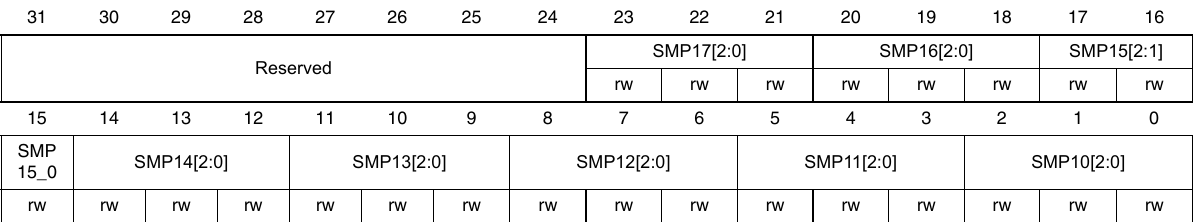
\includegraphics[width=\columnwidth]{./stm32/adc/figs/smpr1.eps}
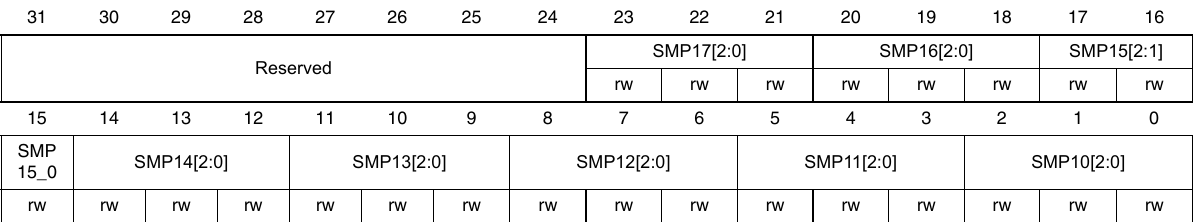
\includegraphics[width=\columnwidth]{./stm32/adc/figs/smpr1}
\caption{SMPR1}
\label{fig:smpr1}
\end{figure}
%
\item What is the sampling time?
\\
\solution Since the sample time is 239.5 cycles and the ADC frequency is 14 MHz, 
\begin{equation}
T_{s} = 239.5 \times \frac{1}{14} \mu s = 17.1 \mu s 
\end{equation}
\item Explain the following instruction.
\begin{lstlisting}
ADC1->SQR3 |= ADC_SQR3_SQ1_4;
\end{lstlisting}

\solution ADC\_SQR3\_SQ1\_4 = 0x00000010.  This implies that SQ1=0b10000 in
the ADC regular sequence register 3 ($ADC1->SQR3$)shown in Fig. \ref{fig:sqr3}. Since SQ1=16,
this means that the ADC input in channel 16 will be the first in the queue
for conversion. 
%
\begin{figure}
\centering
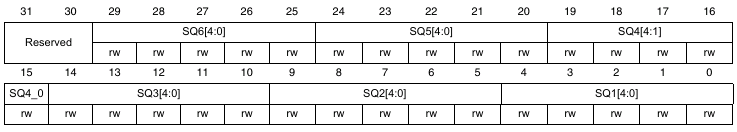
\includegraphics[width=\columnwidth]{./stm32/adc/figs/sqr3}
\caption{SQR3}
\label{fig:sqr3}
\end{figure}
%
The ADC is capable of converting analog 16 inputs one after the other. 
The inputs are called {\em channels} and the sequence number corresponding 
to the channel
is decided
according to the 5 bit entry in SQ. 
\subsection{Measuring an Unkown Resistance}
\item Configure SQR3 so that the 9th channel for ADC1 is 2nd in sequence.
\\
\solution This implies that SQ2=1001.  Thus,
\begin{equation}
ADC1->SQR3 = 0x000000120
\end{equation}
\item List the various pin numbers corresponding to the different channels of the ADC.
\\
\solution See Fig. \ref{table:pin_channel}
%%%%%%%%%%%%%%%%%%%%%%%%%%%%%%%%%%%%%%%%%%%%%%%%%%%%%%%%%%%%%%%%%%%%%%
%%                                                                  %%
%%  This is the header of a LaTeX2e file exported from Gnumeric.    %%
%%                                                                  %%
%%  This file can be compiled as it stands or included in another   %%
%%  LaTeX document. The table is based on the longtable package so  %%
%%  the longtable options (headers, footers...) can be set in the   %%
%%  preamble section below (see PRAMBLE).                           %%
%%                                                                  %%
%%  To include the file in another, the following two lines must be %%
%%  in the including file:                                          %%
%%        \def\inputGnumericTable{}                                 %%
%%  at the beginning of the file and:                               %%
%%        \input{name-of-this-file.tex}                             %%
%%  where the table is to be placed. Note also that the including   %%
%%  file must use the following packages for the table to be        %%
%%  rendered correctly:                                             %%
%%    \usepackage[latin1]{inputenc}                                 %%
%%    \usepackage{color}                                            %%
%%    \usepackage{array}                                            %%
%%    \usepackage{longtable}                                        %%
%%    \usepackage{calc}                                             %%
%%    \usepackage{multirow}                                         %%
%%    \usepackage{hhline}                                           %%
%%    \usepackage{ifthen}                                           %%
%%  optionally (for landscape tables embedded in another document): %%
%%    \usepackage{lscape}                                           %%
%%                                                                  %%
%%%%%%%%%%%%%%%%%%%%%%%%%%%%%%%%%%%%%%%%%%%%%%%%%%%%%%%%%%%%%%%%%%%%%%



%%  This section checks if we are begin input into another file or  %%
%%  the file will be compiled alone. First use a macro taken from   %%
%%  the TeXbook ex 7.7 (suggestion of Han-Wen Nienhuys).            %%
\def\ifundefined#1{\expandafter\ifx\csname#1\endcsname\relax}


%%  Check for the \def token for inputed files. If it is not        %%
%%  defined, the file will be processed as a standalone and the     %%
%%  preamble will be used.                                          %%
\ifundefined{inputGnumericTable}

%%  We must be able to close or not the document at the end.        %%
	\def\gnumericTableEnd{\end{document}}


%%%%%%%%%%%%%%%%%%%%%%%%%%%%%%%%%%%%%%%%%%%%%%%%%%%%%%%%%%%%%%%%%%%%%%
%%                                                                  %%
%%  This is the PREAMBLE. Change these values to get the right      %%
%%  paper size and other niceties.                                  %%
%%                                                                  %%
%%%%%%%%%%%%%%%%%%%%%%%%%%%%%%%%%%%%%%%%%%%%%%%%%%%%%%%%%%%%%%%%%%%%%%

	\documentclass[12pt%
			  %,landscape%
                    ]{report}
       \usepackage[latin1]{inputenc}
       \usepackage{fullpage}
       \usepackage{color}
       \usepackage{array}
       \usepackage{longtable}
       \usepackage{calc}
       \usepackage{multirow}
       \usepackage{hhline}
       \usepackage{ifthen}

	\begin{document}


%%  End of the preamble for the standalone. The next section is for %%
%%  documents which are included into other LaTeX2e files.          %%
\else

%%  We are not a stand alone document. For a regular table, we will %%
%%  have no preamble and only define the closing to mean nothing.   %%
    \def\gnumericTableEnd{}

%%  If we want landscape mode in an embedded document, comment out  %%
%%  the line above and uncomment the two below. The table will      %%
%%  begin on a new page and run in landscape mode.                  %%
%       \def\gnumericTableEnd{\end{landscape}}
%       \begin{landscape}


%%  End of the else clause for this file being \input.              %%
\fi

%%%%%%%%%%%%%%%%%%%%%%%%%%%%%%%%%%%%%%%%%%%%%%%%%%%%%%%%%%%%%%%%%%%%%%
%%                                                                  %%
%%  The rest is the gnumeric table, except for the closing          %%
%%  statement. Changes below will alter the table's appearance.     %%
%%                                                                  %%
%%%%%%%%%%%%%%%%%%%%%%%%%%%%%%%%%%%%%%%%%%%%%%%%%%%%%%%%%%%%%%%%%%%%%%

\providecommand{\gnumericmathit}[1]{#1} 
%%  Uncomment the next line if you would like your numbers to be in %%
%%  italics if they are italizised in the gnumeric table.           %%
%\renewcommand{\gnumericmathit}[1]{\mathit{#1}}
\providecommand{\gnumericPB}[1]%
{\let\gnumericTemp=\\#1\let\\=\gnumericTemp\hspace{0pt}}
 \ifundefined{gnumericTableWidthDefined}
        \newlength{\gnumericTableWidth}
        \newlength{\gnumericTableWidthComplete}
        \newlength{\gnumericMultiRowLength}
        \global\def\gnumericTableWidthDefined{}
 \fi
%% The following setting protects this code from babel shorthands.  %%
 \ifthenelse{\isundefined{\languageshorthands}}{}{\languageshorthands{english}}
%%  The default table format retains the relative column widths of  %%
%%  gnumeric. They can easily be changed to c, r or l. In that case %%
%%  you may want to comment out the next line and uncomment the one %%
%%  thereafter                                                      %%
\providecommand\gnumbox{\makebox[0pt]}
%%\providecommand\gnumbox[1][]{\makebox}

%% to adjust positions in multirow situations                       %%
\setlength{\bigstrutjot}{\jot}
\setlength{\extrarowheight}{\doublerulesep}

%%  The \setlongtables command keeps column widths the same across  %%
%%  pages. Simply comment out next line for varying column widths.  %%
\setlongtables

\setlength\gnumericTableWidth{%
	48pt+%
	24pt+%
	24pt+%
	24pt+%
	24pt+%
	24pt+%
	24pt+%
	24pt+%
	24pt+%
	25pt+%
	25pt+%
0pt}
\def\gumericNumCols{11}
\setlength\gnumericTableWidthComplete{\gnumericTableWidth+%
         \tabcolsep*\gumericNumCols*2+\arrayrulewidth*\gumericNumCols}
\ifthenelse{\lengthtest{\gnumericTableWidthComplete > \linewidth}}%
         {\def\gnumericScale{1*\ratio{\linewidth-%
                        \tabcolsep*\gumericNumCols*2-%
                        \arrayrulewidth*\gumericNumCols}%
{\gnumericTableWidth}}}%
{\def\gnumericScale{1}}

%%%%%%%%%%%%%%%%%%%%%%%%%%%%%%%%%%%%%%%%%%%%%%%%%%%%%%%%%%%%%%%%%%%%%%
%%                                                                  %%
%% The following are the widths of the various columns. We are      %%
%% defining them here because then they are easier to change.       %%
%% Depending on the cell formats we may use them more than once.    %%
%%                                                                  %%
%%%%%%%%%%%%%%%%%%%%%%%%%%%%%%%%%%%%%%%%%%%%%%%%%%%%%%%%%%%%%%%%%%%%%%

\ifthenelse{\isundefined{\gnumericColA}}{\newlength{\gnumericColA}}{}\settowidth{\gnumericColA}{\begin{tabular}{@{}p{48pt*\gnumericScale}@{}}x\end{tabular}}
\ifthenelse{\isundefined{\gnumericColB}}{\newlength{\gnumericColB}}{}\settowidth{\gnumericColB}{\begin{tabular}{@{}p{24pt*\gnumericScale}@{}}x\end{tabular}}
\ifthenelse{\isundefined{\gnumericColC}}{\newlength{\gnumericColC}}{}\settowidth{\gnumericColC}{\begin{tabular}{@{}p{24pt*\gnumericScale}@{}}x\end{tabular}}
\ifthenelse{\isundefined{\gnumericColD}}{\newlength{\gnumericColD}}{}\settowidth{\gnumericColD}{\begin{tabular}{@{}p{24pt*\gnumericScale}@{}}x\end{tabular}}
\ifthenelse{\isundefined{\gnumericColE}}{\newlength{\gnumericColE}}{}\settowidth{\gnumericColE}{\begin{tabular}{@{}p{24pt*\gnumericScale}@{}}x\end{tabular}}
\ifthenelse{\isundefined{\gnumericColF}}{\newlength{\gnumericColF}}{}\settowidth{\gnumericColF}{\begin{tabular}{@{}p{24pt*\gnumericScale}@{}}x\end{tabular}}
\ifthenelse{\isundefined{\gnumericColG}}{\newlength{\gnumericColG}}{}\settowidth{\gnumericColG}{\begin{tabular}{@{}p{24pt*\gnumericScale}@{}}x\end{tabular}}
\ifthenelse{\isundefined{\gnumericColH}}{\newlength{\gnumericColH}}{}\settowidth{\gnumericColH}{\begin{tabular}{@{}p{24pt*\gnumericScale}@{}}x\end{tabular}}
\ifthenelse{\isundefined{\gnumericColI}}{\newlength{\gnumericColI}}{}\settowidth{\gnumericColI}{\begin{tabular}{@{}p{24pt*\gnumericScale}@{}}x\end{tabular}}
\ifthenelse{\isundefined{\gnumericColJ}}{\newlength{\gnumericColJ}}{}\settowidth{\gnumericColJ}{\begin{tabular}{@{}p{25pt*\gnumericScale}@{}}x\end{tabular}}
\ifthenelse{\isundefined{\gnumericColK}}{\newlength{\gnumericColK}}{}\settowidth{\gnumericColK}{\begin{tabular}{@{}p{25pt*\gnumericScale}@{}}x\end{tabular}}

\begin{longtable}[c]{%
	b{\gnumericColA}%
	b{\gnumericColB}%
	b{\gnumericColC}%
	b{\gnumericColD}%
	b{\gnumericColE}%
	b{\gnumericColF}%
	b{\gnumericColG}%
	b{\gnumericColH}%
	b{\gnumericColI}%
	b{\gnumericColJ}%
	b{\gnumericColK}%
	}

%%%%%%%%%%%%%%%%%%%%%%%%%%%%%%%%%%%%%%%%%%%%%%%%%%%%%%%%%%%%%%%%%%%%%%
%%  The longtable options. (Caption, headers... see Goosens, p.124) %%
%	\caption{The Table Caption.}             \\	%

\caption{ADC Analog Input Pins} \label{table:pin_channel}\\
 \hline	% Across the top of the table.
%%  The rest of these options are table rows which are placed on    %%
%%  the first, last or every page. Use \multicolumn if you want.    %%

%%  Header for the first page.                                      %%
%	\multicolumn{11}{c}{The First Header} \\ \hline 
%	\multicolumn{1}{c}{colTag}	%Column 1
%	&\multicolumn{1}{c}{colTag}	%Column 2
%	&\multicolumn{1}{c}{colTag}	%Column 3
%	&\multicolumn{1}{c}{colTag}	%Column 4
%	&\multicolumn{1}{c}{colTag}	%Column 5
%	&\multicolumn{1}{c}{colTag}	%Column 6
%	&\multicolumn{1}{c}{colTag}	%Column 7
%	&\multicolumn{1}{c}{colTag}	%Column 8
%	&\multicolumn{1}{c}{colTag}	%Column 9
%	&\multicolumn{1}{c}{colTag}	%Column 10
%	&\multicolumn{1}{c}{colTag}	\\ \hline %Last column
%	\endfirsthead

%%  The running header definition.                                  %%
%	\hline
%	\multicolumn{11}{l}{\ldots\small\slshape continued} \\ \hline
%	\multicolumn{1}{c}{colTag}	%Column 1
%	&\multicolumn{1}{c}{colTag}	%Column 2
%	&\multicolumn{1}{c}{colTag}	%Column 3
%	&\multicolumn{1}{c}{colTag}	%Column 4
%	&\multicolumn{1}{c}{colTag}	%Column 5
%	&\multicolumn{1}{c}{colTag}	%Column 6
%	&\multicolumn{1}{c}{colTag}	%Column 7
%	&\multicolumn{1}{c}{colTag}	%Column 8
%	&\multicolumn{1}{c}{colTag}	%Column 9
%	&\multicolumn{1}{c}{colTag}	%Column 10
%	&\multicolumn{1}{c}{colTag}	\\ \hline %Last column
%	\endhead

%%  The running footer definition.                                  %%
%	\hline
%	\multicolumn{11}{r}{\small\slshape continued\ldots} \\
%	\endfoot

%%  The ending footer definition.                                   %%
%	\multicolumn{11}{c}{That's all folks} \\ \hline 
%	\endlastfoot
%%%%%%%%%%%%%%%%%%%%%%%%%%%%%%%%%%%%%%%%%%%%%%%%%%%%%%%%%%%%%%%%%%%%%%

\hhline{|-|-|-|-|-|-|-|-|-|-|-}
	 \multicolumn{1}{|p{\gnumericColA}|}%
	{\gnumericPB{\centering}\gnumbox{Channel}}
	&\multicolumn{1}{p{\gnumericColB}|}%
	{\gnumericPB{\centering}\gnumbox{0}}
	&\multicolumn{1}{p{\gnumericColC}|}%
	{\gnumericPB{\centering}\gnumbox{1}}
	&\multicolumn{1}{p{\gnumericColD}|}%
	{\gnumericPB{\centering}\gnumbox{2}}
	&\multicolumn{1}{p{\gnumericColE}|}%
	{\gnumericPB{\centering}\gnumbox{3}}
	&\multicolumn{1}{p{\gnumericColF}|}%
	{\gnumericPB{\centering}\gnumbox{4}}
	&\multicolumn{1}{p{\gnumericColG}|}%
	{\gnumericPB{\centering}\gnumbox{5}}
	&\multicolumn{1}{p{\gnumericColH}|}%
	{\gnumericPB{\centering}\gnumbox{6}}
	&\multicolumn{1}{p{\gnumericColI}|}%
	{\gnumericPB{\centering}\gnumbox{7}}
	&\multicolumn{1}{p{\gnumericColJ}|}%
	{\gnumericPB{\centering}\gnumbox{8}}
	&\multicolumn{1}{p{\gnumericColK}|}%
	{\gnumericPB{\centering}\gnumbox{9}}
\\
\hhline{|-----------|}
	 \multicolumn{1}{|p{\gnumericColA}|}%
	{\gnumericPB{\centering}\gnumbox{Pin}}
	&\multicolumn{1}{p{\gnumericColB}|}%
	{\gnumericPB{\centering}\gnumbox{PA0}}
	&\multicolumn{1}{p{\gnumericColC}|}%
	{\gnumericPB{\centering}\gnumbox{PA1}}
	&\multicolumn{1}{p{\gnumericColD}|}%
	{\gnumericPB{\centering}\gnumbox{PA2}}
	&\multicolumn{1}{p{\gnumericColE}|}%
	{\gnumericPB{\centering}\gnumbox{PA3}}
	&\multicolumn{1}{p{\gnumericColF}|}%
	{\gnumericPB{\centering}\gnumbox{PA4}}
	&\multicolumn{1}{p{\gnumericColG}|}%
	{\gnumericPB{\centering}\gnumbox{PA5}}
	&\multicolumn{1}{p{\gnumericColH}|}%
	{\gnumericPB{\centering}\gnumbox{PA6}}
	&\multicolumn{1}{p{\gnumericColI}|}%
	{\gnumericPB{\centering}\gnumbox{PA7}}
	&\multicolumn{1}{p{\gnumericColJ}|}%
	{\gnumericPB{\centering}\gnumbox{PB0}}
	&\multicolumn{1}{p{\gnumericColK}|}%
	{\gnumericPB{\centering}\gnumbox{PB1}}
\\
\hhline{|-|-|-|-|-|-|-|-|-|-|-|}
\end{longtable}

\ifthenelse{\isundefined{\languageshorthands}}{}{\languageshorthands{\languagename}}
\gnumericTableEnd

\iffalse
\begin{table}[!ht]
\footnotesize
%%%%%%%%%%%%%%%%%%%%%%%%%%%%%%%%%%%%%%%%%%%%%%%%%%%%%%%%%%%%%%%%%%%%%%
%%                                                                  %%
%%  This is the header of a LaTeX2e file exported from Gnumeric.    %%
%%                                                                  %%
%%  This file can be compiled as it stands or included in another   %%
%%  LaTeX document. The table is based on the longtable package so  %%
%%  the longtable options (headers, footers...) can be set in the   %%
%%  preamble section below (see PRAMBLE).                           %%
%%                                                                  %%
%%  To include the file in another, the following two lines must be %%
%%  in the including file:                                          %%
%%        \def\inputGnumericTable{}                                 %%
%%  at the beginning of the file and:                               %%
%%        \input{name-of-this-file.tex}                             %%
%%  where the table is to be placed. Note also that the including   %%
%%  file must use the following packages for the table to be        %%
%%  rendered correctly:                                             %%
%%    \usepackage[latin1]{inputenc}                                 %%
%%    \usepackage{color}                                            %%
%%    \usepackage{array}                                            %%
%%    \usepackage{longtable}                                        %%
%%    \usepackage{calc}                                             %%
%%    \usepackage{multirow}                                         %%
%%    \usepackage{hhline}                                           %%
%%    \usepackage{ifthen}                                           %%
%%  optionally (for landscape tables embedded in another document): %%
%%    \usepackage{lscape}                                           %%
%%                                                                  %%
%%%%%%%%%%%%%%%%%%%%%%%%%%%%%%%%%%%%%%%%%%%%%%%%%%%%%%%%%%%%%%%%%%%%%%



%%  This section checks if we are begin input into another file or  %%
%%  the file will be compiled alone. First use a macro taken from   %%
%%  the TeXbook ex 7.7 (suggestion of Han-Wen Nienhuys).            %%
\def\ifundefined#1{\expandafter\ifx\csname#1\endcsname\relax}


%%  Check for the \def token for inputed files. If it is not        %%
%%  defined, the file will be processed as a standalone and the     %%
%%  preamble will be used.                                          %%
\ifundefined{inputGnumericTable}

%%  We must be able to close or not the document at the end.        %%
	\def\gnumericTableEnd{\end{document}}


%%%%%%%%%%%%%%%%%%%%%%%%%%%%%%%%%%%%%%%%%%%%%%%%%%%%%%%%%%%%%%%%%%%%%%
%%                                                                  %%
%%  This is the PREAMBLE. Change these values to get the right      %%
%%  paper size and other niceties.                                  %%
%%                                                                  %%
%%%%%%%%%%%%%%%%%%%%%%%%%%%%%%%%%%%%%%%%%%%%%%%%%%%%%%%%%%%%%%%%%%%%%%

	\documentclass[12pt%
			  %,landscape%
                    ]{report}
       \usepackage[latin1]{inputenc}
       \usepackage{fullpage}
       \usepackage{color}
       \usepackage{array}
       \usepackage{longtable}
       \usepackage{calc}
       \usepackage{multirow}
       \usepackage{hhline}
       \usepackage{ifthen}

	\begin{document}


%%  End of the preamble for the standalone. The next section is for %%
%%  documents which are included into other LaTeX2e files.          %%
\else

%%  We are not a stand alone document. For a regular table, we will %%
%%  have no preamble and only define the closing to mean nothing.   %%
    \def\gnumericTableEnd{}

%%  If we want landscape mode in an embedded document, comment out  %%
%%  the line above and uncomment the two below. The table will      %%
%%  begin on a new page and run in landscape mode.                  %%
%       \def\gnumericTableEnd{\end{landscape}}
%       \begin{landscape}


%%  End of the else clause for this file being \input.              %%
\fi

%%%%%%%%%%%%%%%%%%%%%%%%%%%%%%%%%%%%%%%%%%%%%%%%%%%%%%%%%%%%%%%%%%%%%%
%%                                                                  %%
%%  The rest is the gnumeric table, except for the closing          %%
%%  statement. Changes below will alter the table's appearance.     %%
%%                                                                  %%
%%%%%%%%%%%%%%%%%%%%%%%%%%%%%%%%%%%%%%%%%%%%%%%%%%%%%%%%%%%%%%%%%%%%%%

\providecommand{\gnumericmathit}[1]{#1} 
%%  Uncomment the next line if you would like your numbers to be in %%
%%  italics if they are italizised in the gnumeric table.           %%
%\renewcommand{\gnumericmathit}[1]{\mathit{#1}}
\providecommand{\gnumericPB}[1]%
{\let\gnumericTemp=\\#1\let\\=\gnumericTemp\hspace{0pt}}
 \ifundefined{gnumericTableWidthDefined}
        \newlength{\gnumericTableWidth}
        \newlength{\gnumericTableWidthComplete}
        \newlength{\gnumericMultiRowLength}
        \global\def\gnumericTableWidthDefined{}
 \fi
%% The following setting protects this code from babel shorthands.  %%
 \ifthenelse{\isundefined{\languageshorthands}}{}{\languageshorthands{english}}
%%  The default table format retains the relative column widths of  %%
%%  gnumeric. They can easily be changed to c, r or l. In that case %%
%%  you may want to comment out the next line and uncomment the one %%
%%  thereafter                                                      %%
\providecommand\gnumbox{\makebox[0pt]}
%%\providecommand\gnumbox[1][]{\makebox}

%% to adjust positions in multirow situations                       %%
\setlength{\bigstrutjot}{\jot}
\setlength{\extrarowheight}{\doublerulesep}

%%  The \setlongtables command keeps column widths the same across  %%
%%  pages. Simply comment out next line for varying column widths.  %%
\setlongtables

\setlength\gnumericTableWidth{%
	48pt+%
	24pt+%
	24pt+%
	24pt+%
	24pt+%
	24pt+%
	24pt+%
	24pt+%
	24pt+%
	25pt+%
	25pt+%
0pt}
\def\gumericNumCols{11}
\setlength\gnumericTableWidthComplete{\gnumericTableWidth+%
         \tabcolsep*\gumericNumCols*2+\arrayrulewidth*\gumericNumCols}
\ifthenelse{\lengthtest{\gnumericTableWidthComplete > \linewidth}}%
         {\def\gnumericScale{1*\ratio{\linewidth-%
                        \tabcolsep*\gumericNumCols*2-%
                        \arrayrulewidth*\gumericNumCols}%
{\gnumericTableWidth}}}%
{\def\gnumericScale{1}}

%%%%%%%%%%%%%%%%%%%%%%%%%%%%%%%%%%%%%%%%%%%%%%%%%%%%%%%%%%%%%%%%%%%%%%
%%                                                                  %%
%% The following are the widths of the various columns. We are      %%
%% defining them here because then they are easier to change.       %%
%% Depending on the cell formats we may use them more than once.    %%
%%                                                                  %%
%%%%%%%%%%%%%%%%%%%%%%%%%%%%%%%%%%%%%%%%%%%%%%%%%%%%%%%%%%%%%%%%%%%%%%

\ifthenelse{\isundefined{\gnumericColA}}{\newlength{\gnumericColA}}{}\settowidth{\gnumericColA}{\begin{tabular}{@{}p{48pt*\gnumericScale}@{}}x\end{tabular}}
\ifthenelse{\isundefined{\gnumericColB}}{\newlength{\gnumericColB}}{}\settowidth{\gnumericColB}{\begin{tabular}{@{}p{24pt*\gnumericScale}@{}}x\end{tabular}}
\ifthenelse{\isundefined{\gnumericColC}}{\newlength{\gnumericColC}}{}\settowidth{\gnumericColC}{\begin{tabular}{@{}p{24pt*\gnumericScale}@{}}x\end{tabular}}
\ifthenelse{\isundefined{\gnumericColD}}{\newlength{\gnumericColD}}{}\settowidth{\gnumericColD}{\begin{tabular}{@{}p{24pt*\gnumericScale}@{}}x\end{tabular}}
\ifthenelse{\isundefined{\gnumericColE}}{\newlength{\gnumericColE}}{}\settowidth{\gnumericColE}{\begin{tabular}{@{}p{24pt*\gnumericScale}@{}}x\end{tabular}}
\ifthenelse{\isundefined{\gnumericColF}}{\newlength{\gnumericColF}}{}\settowidth{\gnumericColF}{\begin{tabular}{@{}p{24pt*\gnumericScale}@{}}x\end{tabular}}
\ifthenelse{\isundefined{\gnumericColG}}{\newlength{\gnumericColG}}{}\settowidth{\gnumericColG}{\begin{tabular}{@{}p{24pt*\gnumericScale}@{}}x\end{tabular}}
\ifthenelse{\isundefined{\gnumericColH}}{\newlength{\gnumericColH}}{}\settowidth{\gnumericColH}{\begin{tabular}{@{}p{24pt*\gnumericScale}@{}}x\end{tabular}}
\ifthenelse{\isundefined{\gnumericColI}}{\newlength{\gnumericColI}}{}\settowidth{\gnumericColI}{\begin{tabular}{@{}p{24pt*\gnumericScale}@{}}x\end{tabular}}
\ifthenelse{\isundefined{\gnumericColJ}}{\newlength{\gnumericColJ}}{}\settowidth{\gnumericColJ}{\begin{tabular}{@{}p{25pt*\gnumericScale}@{}}x\end{tabular}}
\ifthenelse{\isundefined{\gnumericColK}}{\newlength{\gnumericColK}}{}\settowidth{\gnumericColK}{\begin{tabular}{@{}p{25pt*\gnumericScale}@{}}x\end{tabular}}

\begin{longtable}[c]{%
	b{\gnumericColA}%
	b{\gnumericColB}%
	b{\gnumericColC}%
	b{\gnumericColD}%
	b{\gnumericColE}%
	b{\gnumericColF}%
	b{\gnumericColG}%
	b{\gnumericColH}%
	b{\gnumericColI}%
	b{\gnumericColJ}%
	b{\gnumericColK}%
	}

%%%%%%%%%%%%%%%%%%%%%%%%%%%%%%%%%%%%%%%%%%%%%%%%%%%%%%%%%%%%%%%%%%%%%%
%%  The longtable options. (Caption, headers... see Goosens, p.124) %%
%	\caption{The Table Caption.}             \\	%

\caption{ADC Analog Input Pins} \label{table:pin_channel}\\
 \hline	% Across the top of the table.
%%  The rest of these options are table rows which are placed on    %%
%%  the first, last or every page. Use \multicolumn if you want.    %%

%%  Header for the first page.                                      %%
%	\multicolumn{11}{c}{The First Header} \\ \hline 
%	\multicolumn{1}{c}{colTag}	%Column 1
%	&\multicolumn{1}{c}{colTag}	%Column 2
%	&\multicolumn{1}{c}{colTag}	%Column 3
%	&\multicolumn{1}{c}{colTag}	%Column 4
%	&\multicolumn{1}{c}{colTag}	%Column 5
%	&\multicolumn{1}{c}{colTag}	%Column 6
%	&\multicolumn{1}{c}{colTag}	%Column 7
%	&\multicolumn{1}{c}{colTag}	%Column 8
%	&\multicolumn{1}{c}{colTag}	%Column 9
%	&\multicolumn{1}{c}{colTag}	%Column 10
%	&\multicolumn{1}{c}{colTag}	\\ \hline %Last column
%	\endfirsthead

%%  The running header definition.                                  %%
%	\hline
%	\multicolumn{11}{l}{\ldots\small\slshape continued} \\ \hline
%	\multicolumn{1}{c}{colTag}	%Column 1
%	&\multicolumn{1}{c}{colTag}	%Column 2
%	&\multicolumn{1}{c}{colTag}	%Column 3
%	&\multicolumn{1}{c}{colTag}	%Column 4
%	&\multicolumn{1}{c}{colTag}	%Column 5
%	&\multicolumn{1}{c}{colTag}	%Column 6
%	&\multicolumn{1}{c}{colTag}	%Column 7
%	&\multicolumn{1}{c}{colTag}	%Column 8
%	&\multicolumn{1}{c}{colTag}	%Column 9
%	&\multicolumn{1}{c}{colTag}	%Column 10
%	&\multicolumn{1}{c}{colTag}	\\ \hline %Last column
%	\endhead

%%  The running footer definition.                                  %%
%	\hline
%	\multicolumn{11}{r}{\small\slshape continued\ldots} \\
%	\endfoot

%%  The ending footer definition.                                   %%
%	\multicolumn{11}{c}{That's all folks} \\ \hline 
%	\endlastfoot
%%%%%%%%%%%%%%%%%%%%%%%%%%%%%%%%%%%%%%%%%%%%%%%%%%%%%%%%%%%%%%%%%%%%%%

\hhline{|-|-|-|-|-|-|-|-|-|-|-}
	 \multicolumn{1}{|p{\gnumericColA}|}%
	{\gnumericPB{\centering}\gnumbox{Channel}}
	&\multicolumn{1}{p{\gnumericColB}|}%
	{\gnumericPB{\centering}\gnumbox{0}}
	&\multicolumn{1}{p{\gnumericColC}|}%
	{\gnumericPB{\centering}\gnumbox{1}}
	&\multicolumn{1}{p{\gnumericColD}|}%
	{\gnumericPB{\centering}\gnumbox{2}}
	&\multicolumn{1}{p{\gnumericColE}|}%
	{\gnumericPB{\centering}\gnumbox{3}}
	&\multicolumn{1}{p{\gnumericColF}|}%
	{\gnumericPB{\centering}\gnumbox{4}}
	&\multicolumn{1}{p{\gnumericColG}|}%
	{\gnumericPB{\centering}\gnumbox{5}}
	&\multicolumn{1}{p{\gnumericColH}|}%
	{\gnumericPB{\centering}\gnumbox{6}}
	&\multicolumn{1}{p{\gnumericColI}|}%
	{\gnumericPB{\centering}\gnumbox{7}}
	&\multicolumn{1}{p{\gnumericColJ}|}%
	{\gnumericPB{\centering}\gnumbox{8}}
	&\multicolumn{1}{p{\gnumericColK}|}%
	{\gnumericPB{\centering}\gnumbox{9}}
\\
\hhline{|-----------|}
	 \multicolumn{1}{|p{\gnumericColA}|}%
	{\gnumericPB{\centering}\gnumbox{Pin}}
	&\multicolumn{1}{p{\gnumericColB}|}%
	{\gnumericPB{\centering}\gnumbox{PA0}}
	&\multicolumn{1}{p{\gnumericColC}|}%
	{\gnumericPB{\centering}\gnumbox{PA1}}
	&\multicolumn{1}{p{\gnumericColD}|}%
	{\gnumericPB{\centering}\gnumbox{PA2}}
	&\multicolumn{1}{p{\gnumericColE}|}%
	{\gnumericPB{\centering}\gnumbox{PA3}}
	&\multicolumn{1}{p{\gnumericColF}|}%
	{\gnumericPB{\centering}\gnumbox{PA4}}
	&\multicolumn{1}{p{\gnumericColG}|}%
	{\gnumericPB{\centering}\gnumbox{PA5}}
	&\multicolumn{1}{p{\gnumericColH}|}%
	{\gnumericPB{\centering}\gnumbox{PA6}}
	&\multicolumn{1}{p{\gnumericColI}|}%
	{\gnumericPB{\centering}\gnumbox{PA7}}
	&\multicolumn{1}{p{\gnumericColJ}|}%
	{\gnumericPB{\centering}\gnumbox{PB0}}
	&\multicolumn{1}{p{\gnumericColK}|}%
	{\gnumericPB{\centering}\gnumbox{PB1}}
\\
\hhline{|-|-|-|-|-|-|-|-|-|-|-|}
\end{longtable}

\ifthenelse{\isundefined{\languageshorthands}}{}{\languageshorthands{\languagename}}
\gnumericTableEnd

\caption{ADC Analog Input Pins}
\label{table:pin_channel}
\end{table}
\fi
\item Use the 9th channel of  ADC1 in SQ2 to measure 3.3V. 
\\
\solution Connect PB1 (Fig. \ref{table:pin_channel}) to 3.3 V of the STM 32 and execute the following
code.
\begin{lstlisting}
stm32/adc/codes/3_3V.c
\end{lstlisting}
%\section{Project}
\item Measure an unkown resistance using the STM32 and display the result on the LCD.
\item Display the output of the internal temperature sensor as well the unknown resistance on the LCD.
\end{enumerate}


\newpage
\appendices
\newpage
\section{PicoW}
\subsection{Arduino Framework}
\begin{enumerate}[label=\arabic*.,ref=\theenumi]
	\item The following instructions are for the picow toolchain
		in termux-debian
		\label{it:picow/installation/toolchain}
\begin{lstlisting}
cd .platformio/packages
git clone https://github.com/earlephilhower/arduino-pico
cd arduino-pico
git submodule update --init
cd pico-sdk
git submodule update --init
cd ../tools
python3 ./get.py
\end{lstlisting}
\item Downlaod EtchDroid from F-DROID. 
\item Now execute the following 
\label{it:picow/installation/toolchain/rpi}
\begin{lstlisting}
cd picow/ide/codes/
pio run
cp .pio/build/rpipicow/firmware.uf2 /sdcard/Download/
\end{lstlisting}
\item  Keep BOOTSEL pressed on picow  and connect it to your phone.
\item Now flash picow using EtchDroid.
\item The Onboard LED will start blinking.
\item Change the blink frequency.
\item If Item \ref{it:picow/installation/toolchain} is unsuccessful, 
\begin{enumerate}
	\item
		Execute Item
\ref{it:picow/installation/toolchain/rpi}
on your rpi
	\item Copy relevant platformio packages from your raspberry pi to your phone .platformio/packages directory using scp.
\end{enumerate}
\item 
	See
			\figref{fig:picowpinout} for the picow pin diagram.
			You may reuse all the Arduino codes for pico by changing only the platformio.ini file.
% Insert your image here
		\begin{figure}
			\centering
    \includegraphics[width=\columnwidth]{picow/installation/figs/picowpinout.jpg}
    \caption{PICOW Pin Diagram} % Adds a centered caption under the image
			\label{fig:picowpinout}
		\end{figure}
%\item Connect RUN on pico W to GND. Keep pressing BOOTSEL while removing the RUN-GND wire from GND.Pico W is now ready to be flashed.
\end{enumerate}


\iffalse
\subsection{Seven Segment Display}
\begin{enumerate}[label=\arabic*.,ref=\theenumi]
\item
Make connections according to Table \ref{table:esp-ard_disp_num}
%\iffalse
\begin{table}[H]
\centering
\input{esp32/ide/sevenseg/figs/ard_disp_num}
\caption{}
\label{table:esp-ard_disp_num}
\end{table}
%\fi

\item
Execute the following
%
\begin{lstlisting}
esp32/ide/sevenseg/src/main.cpp
\end{lstlisting}
%
The number 5 should be displayed.
\item
Now generate the numbers 0-9 by modifying the above program.

\end{enumerate}

\subsection{7447}
\begin{enumerate}[label=\arabic*.,ref=\theenumi]
\item
Make connections according to Table \ref{table:esp-ard_disp_num}
%\iffalse
\begin{table}[H]
\centering
\input{esp32/ide/sevenseg/figs/ard_disp_num}
\caption{}
\label{table:esp-ard_disp_num}
\end{table}
%\fi

\item
Execute the following
%
\begin{lstlisting}
esp32/ide/sevenseg/src/main.cpp
\end{lstlisting}
%
The number 5 should be displayed.
\item
Now generate the numbers 0-9 by modifying the above program.

\end{enumerate}

%\subsection{Problems}
%\begin{enumerate}[label=\arabic*.,ref=\theenumi]
\item In a given $8$-bit general purpose micro-controller there are following flags. $C$-Carry, $A$-Auxiliary Carry, $O$-Overflow flag, $P$-Parity ($0$ for even, $1$ for odd) $R0$ and $R1$ are the two general purpose registers of the micro-controller. After execution of the following instructions, the decimal equivalent of the binary sequence of the flag pattern $[CAOP]$ will be \rule{1cm}{0.1pt}.
\hfill{(GATE EE 2023)}
\begin{lstlisting}
MOV R0,+0x60
MOV R1,+0x46 
ADD R0,R1
\end{lstlisting}
\item 
Consider the given C-code and its corresponding assembly code, with a few operands U1-U4 being unknown. Some useful information as well as the semantics of each unique assembly instruction is annotated as inline comments in the code.
\begin{lstlisting}
int a[10],b[10],i;
//int is 32-bit
for (i=0;i<10;i++)
a[i]=b[i]*8;
\end{lstlisting}
%
\begin{lstlisting}
;r1-r5 are 32-bit integer registers
;initialize r1=0,r2=0
;initialize r3,r4 with base address of a,b

L01:jeq r1,r2,end ;if(r1==r2) goto end
L02:lw r5,0(r4)   ;r5<-Memory[r4+0]
L03:shl r5,r5,U1  ;r5<-r5<<U1
L04:sw r5,0(r3)   ;Memory[r3+0]<- r5
L05:add r3,r3,U2  ;r3<-r3+U2
L06:add r4,r4,U3
L07:add r1,r1,1
L08:jmp U4        ;goto U4
L09:end
\end{lstlisting}
Which one of the following options is a CORRECT replacement 
for operands in the position (U1,U2,U3,U4) in the above 
assembly code?
%
\begin{multicols}{2}
\begin{enumerate}
\item (8,4,1,L02)                      
\item (3,4,4,L01)
\item (8,1,1,L02)                             
\item (3,1,1,L01)         
\end{enumerate}
\end{multicols}
\item An $8085$ microprocessor accesses two memory locations $\brak{2001H}$ and $\brak{2002H}$, that contain $8$-bit numbers $98$H and $B1$H, respectively.The following program is executed:
\begin{verbatim}LXI H,2001H
MVI A,21H
INX H
ADD M
INX H
MOV M,A
HLT
\end{verbatim}
		At the end of this program, the memory location $2003$H contains the number in decimal form \rule{1cm}{0.1pt}.
		\hfill (GATE EE 2020)
\item  Which of the following is the correct binary equivalent of the hexadecimal F6C?
	\hfill (GATE PH 2020)
%
\begin{multicols}{2}
\begin{enumerate}
  \item  $0110 1111 1100$
  \item $1111 0110 1100$
  \item $1100 0110 1111$
  \item $0110 1100 0111$
\end{enumerate}
\end{multicols}
\item
\label{prob:gate IN 45}
 A portion of an assembly language program written for an $8$-bit microprocessor is given below along with explanations. The code is intended to introduce a software time delay. The processor is driven by a $5$ MHz clock. The time delay (in $\mu$s) introduced by the program is 
\hfill(GATE IN 2018)
\begin{lstlisting}
MVI B, $64$H; Move immediate the given byte into register B. Takes 7 clock periods.
LOOP: DCR B ; Decrement register B. Affects Flags. Takes 4 clock periods. 
JNZ LOOP ; Jump to address with Label LOOP if zero flag is not set. Takes 10 clock periods when jump is performed and 7 clock periods when jump is not performed.
\end{lstlisting}
%
\item A $10\frac{1}{2}$ digit Counter-timer is set in the `frequency mode' of operation (with $T_s=1s$). For a specific input, the reading obtained is $1000$. Without disconnecting this input, the Counter-timer is changed to operate in the `Period mode' and the range selected is microseconds ($\mu$s, with $f_s=\SI{1}{\mega\hertz}$).The Counter will then display
\begin{multicols}{4}
\begin{enumerate}
  \item $0$
  \item $10$
  \item $100$
  \item $1000$
\end{enumerate}
\end{multicols}
\hfill(GATE IN 2021)

\item Consider three registers R1 ,R2 ,R3 that store numbers in  IEEE-754  single precision floating point format. Assume that R1 and R2 contain the values (in hexadecimal notation) 0x42200000 and 0xC1200000, respectively. If  R3=$\frac{\text{R1}}{\text{R2}}$, what is the value stored in R3?
\hfill(GATE EC 2021)
\begin{multicols}{2}
\begin{enumerate}
    \item 0x40800000
    \item 0xC0800000
    \item 0x83400000
    \item 0xC8500000
\end{enumerate}
\end{multicols}
%
\item The content of the registers are $R_1 = 25H$, $R_2 = 30H$ and $R_3 = 40H$. The following machine instructions are executed.
	\begin{lstlisting}
  PUSH R1  
  PUSH R2
  PUSH R3 
  POP R1 
  POP R2 
  POP R3 
\end{lstlisting}
%
After execution, the content of registers R1, R2, R3 are
\hfill(GATE EC 2021)
%
\begin{multicols}{2}
\begin{enumerate}
    \item $R_1 = 40H, R_2 = 30H,R_3 = 25H$
    \item $R_1 = 25H, R_2 = 30H,R_3 = 40H$
    \item $R_1 = 30H, R_2 = 40H,R_3 = 25H$
    \item $R_1 = 40H, R_2 = 25H,R_3 = 30H$
\end{enumerate}
\end{multicols}
\end{enumerate}

\subsection{Karnaugh Map}
\subsection{ Incrementing Decoder}
\begin{enumerate}[label=\arabic*.,ref=\theenumi]
\item
Make connections according to Table \ref{table:esp-ard_disp_num}
%\iffalse
\begin{table}[H]
\centering
\input{esp32/ide/sevenseg/figs/ard_disp_num}
\caption{}
\label{table:esp-ard_disp_num}
\end{table}
%\fi

\item
Execute the following
%
\begin{lstlisting}
esp32/ide/sevenseg/src/main.cpp
\end{lstlisting}
%
The number 5 should be displayed.
\item
Now generate the numbers 0-9 by modifying the above program.

\end{enumerate}

\subsection{Dont Care}
\begin{enumerate}[label=\arabic*.,ref=\theenumi]
\item
Make connections according to Table \ref{table:esp-ard_disp_num}
%\iffalse
\begin{table}[H]
\centering
\input{esp32/ide/sevenseg/figs/ard_disp_num}
\caption{}
\label{table:esp-ard_disp_num}
\end{table}
%\fi

\item
Execute the following
%
\begin{lstlisting}
esp32/ide/sevenseg/src/main.cpp
\end{lstlisting}
%
The number 5 should be displayed.
\item
Now generate the numbers 0-9 by modifying the above program.

\end{enumerate}

%\subsection{Problems}
%\begin{enumerate}[label=\arabic*.,ref=\theenumi]
\item In a given $8$-bit general purpose micro-controller there are following flags. $C$-Carry, $A$-Auxiliary Carry, $O$-Overflow flag, $P$-Parity ($0$ for even, $1$ for odd) $R0$ and $R1$ are the two general purpose registers of the micro-controller. After execution of the following instructions, the decimal equivalent of the binary sequence of the flag pattern $[CAOP]$ will be \rule{1cm}{0.1pt}.
\hfill{(GATE EE 2023)}
\begin{lstlisting}
MOV R0,+0x60
MOV R1,+0x46 
ADD R0,R1
\end{lstlisting}
\item 
Consider the given C-code and its corresponding assembly code, with a few operands U1-U4 being unknown. Some useful information as well as the semantics of each unique assembly instruction is annotated as inline comments in the code.
\begin{lstlisting}
int a[10],b[10],i;
//int is 32-bit
for (i=0;i<10;i++)
a[i]=b[i]*8;
\end{lstlisting}
%
\begin{lstlisting}
;r1-r5 are 32-bit integer registers
;initialize r1=0,r2=0
;initialize r3,r4 with base address of a,b

L01:jeq r1,r2,end ;if(r1==r2) goto end
L02:lw r5,0(r4)   ;r5<-Memory[r4+0]
L03:shl r5,r5,U1  ;r5<-r5<<U1
L04:sw r5,0(r3)   ;Memory[r3+0]<- r5
L05:add r3,r3,U2  ;r3<-r3+U2
L06:add r4,r4,U3
L07:add r1,r1,1
L08:jmp U4        ;goto U4
L09:end
\end{lstlisting}
Which one of the following options is a CORRECT replacement 
for operands in the position (U1,U2,U3,U4) in the above 
assembly code?
%
\begin{multicols}{2}
\begin{enumerate}
\item (8,4,1,L02)                      
\item (3,4,4,L01)
\item (8,1,1,L02)                             
\item (3,1,1,L01)         
\end{enumerate}
\end{multicols}
\item An $8085$ microprocessor accesses two memory locations $\brak{2001H}$ and $\brak{2002H}$, that contain $8$-bit numbers $98$H and $B1$H, respectively.The following program is executed:
\begin{verbatim}LXI H,2001H
MVI A,21H
INX H
ADD M
INX H
MOV M,A
HLT
\end{verbatim}
		At the end of this program, the memory location $2003$H contains the number in decimal form \rule{1cm}{0.1pt}.
		\hfill (GATE EE 2020)
\item  Which of the following is the correct binary equivalent of the hexadecimal F6C?
	\hfill (GATE PH 2020)
%
\begin{multicols}{2}
\begin{enumerate}
  \item  $0110 1111 1100$
  \item $1111 0110 1100$
  \item $1100 0110 1111$
  \item $0110 1100 0111$
\end{enumerate}
\end{multicols}
\item
\label{prob:gate IN 45}
 A portion of an assembly language program written for an $8$-bit microprocessor is given below along with explanations. The code is intended to introduce a software time delay. The processor is driven by a $5$ MHz clock. The time delay (in $\mu$s) introduced by the program is 
\hfill(GATE IN 2018)
\begin{lstlisting}
MVI B, $64$H; Move immediate the given byte into register B. Takes 7 clock periods.
LOOP: DCR B ; Decrement register B. Affects Flags. Takes 4 clock periods. 
JNZ LOOP ; Jump to address with Label LOOP if zero flag is not set. Takes 10 clock periods when jump is performed and 7 clock periods when jump is not performed.
\end{lstlisting}
%
\item A $10\frac{1}{2}$ digit Counter-timer is set in the `frequency mode' of operation (with $T_s=1s$). For a specific input, the reading obtained is $1000$. Without disconnecting this input, the Counter-timer is changed to operate in the `Period mode' and the range selected is microseconds ($\mu$s, with $f_s=\SI{1}{\mega\hertz}$).The Counter will then display
\begin{multicols}{4}
\begin{enumerate}
  \item $0$
  \item $10$
  \item $100$
  \item $1000$
\end{enumerate}
\end{multicols}
\hfill(GATE IN 2021)

\item Consider three registers R1 ,R2 ,R3 that store numbers in  IEEE-754  single precision floating point format. Assume that R1 and R2 contain the values (in hexadecimal notation) 0x42200000 and 0xC1200000, respectively. If  R3=$\frac{\text{R1}}{\text{R2}}$, what is the value stored in R3?
\hfill(GATE EC 2021)
\begin{multicols}{2}
\begin{enumerate}
    \item 0x40800000
    \item 0xC0800000
    \item 0x83400000
    \item 0xC8500000
\end{enumerate}
\end{multicols}
%
\item The content of the registers are $R_1 = 25H$, $R_2 = 30H$ and $R_3 = 40H$. The following machine instructions are executed.
	\begin{lstlisting}
  PUSH R1  
  PUSH R2
  PUSH R3 
  POP R1 
  POP R2 
  POP R3 
\end{lstlisting}
%
After execution, the content of registers R1, R2, R3 are
\hfill(GATE EC 2021)
%
\begin{multicols}{2}
\begin{enumerate}
    \item $R_1 = 40H, R_2 = 30H,R_3 = 25H$
    \item $R_1 = 25H, R_2 = 30H,R_3 = 40H$
    \item $R_1 = 30H, R_2 = 40H,R_3 = 25H$
    \item $R_1 = 40H, R_2 = 25H,R_3 = 30H$
\end{enumerate}
\end{multicols}
\end{enumerate}

\subsection{7474}
\begin{enumerate}[label=\arabic*.,ref=\theenumi]
\item
Make connections according to Table \ref{table:esp-ard_disp_num}
%\iffalse
\begin{table}[H]
\centering
\input{esp32/ide/sevenseg/figs/ard_disp_num}
\caption{}
\label{table:esp-ard_disp_num}
\end{table}
%\fi

\item
Execute the following
%
\begin{lstlisting}
esp32/ide/sevenseg/src/main.cpp
\end{lstlisting}
%
The number 5 should be displayed.
\item
Now generate the numbers 0-9 by modifying the above program.

\end{enumerate}

\fi




\section{Pico}
\subsection{Setup}
\begin{enumerate}[label=\arabic*.,ref=\theenumi]
\item
Make connections according to Table \ref{table:esp-ard_disp_num}
%\iffalse
\begin{table}[H]
\centering
\input{esp32/ide/sevenseg/figs/ard_disp_num}
\caption{}
\label{table:esp-ard_disp_num}
\end{table}
%\fi

\item
Execute the following
%
\begin{lstlisting}
esp32/ide/sevenseg/src/main.cpp
\end{lstlisting}
%
The number 5 should be displayed.
\item
Now generate the numbers 0-9 by modifying the above program.

\end{enumerate}

%
%\section{Wired Protocols}
%\subsection{UART}
%\begin{enumerate}[label=\arabic*.,ref=\theenumi]
\item
Make connections according to Table \ref{table:esp-ard_disp_num}
%\iffalse
\begin{table}[H]
\centering
\input{esp32/ide/sevenseg/figs/ard_disp_num}
\caption{}
\label{table:esp-ard_disp_num}
\end{table}
%\fi

\item
Execute the following
%
\begin{lstlisting}
esp32/ide/sevenseg/src/main.cpp
\end{lstlisting}
%
The number 5 should be displayed.
\item
Now generate the numbers 0-9 by modifying the above program.

\end{enumerate}

\end{document}
